\documentclass[10pt,oneside]{book}

\usepackage{cdt/cdtUsecases}
\usepackage{txfonts}


% !TeX root = proyecto.tex

\definecolor{coverBlue}{RGB}{21,96,130}

% Pie de página: el encabezado queda vacío en todo el documento.
\fancyhf{}
\fancyfoot[C]{\footnotesize pág. \thepage}
\renewcommand{\headrulewidth}{0pt}
\renewcommand{\footrulewidth}{0pt}
\fancypagestyle{documentplain}{%
\fancyhf{}
\fancyfoot[C]{\footnotesize pág. \thepage}
\renewcommand{\headrulewidth}{0pt}
\renewcommand{\footrulewidth}{0pt}
}
\fancypagestyle{indexplain}{%
\fancyhf{}
\renewcommand{\headrulewidth}{0pt}
\renewcommand{\footrulewidth}{0pt}
}
\makeatletter
\let\ps@plain\ps@documentplain
\makeatother


%=========================================================
% Datos del documento:
\defProyecto{Sistema de Gestión de Cocina (KMS) para la Optimización de Pedidos y Procesos en Cafeterías del Instituto Politécnico Nacional, Unidad Zacatenco}
\defNumComponente{Componente 2}
\defComponente{Documento de análisis}
\defEtapa{Etapa del documento: etapa 0}

%=========================================================
% Datos de la consultora:
\defConsultora{Hernández Jiménez Erick Yael, Miranda San Martin Angel, Robert Garayzar Arturo}
\defNomSupervisor{}
\defCargoSupervisor{}

%=========================================================
% Datos del cliente:
\defCliente{Trabajo Terminal I}
\defNomResponsable{Instituto Politécnico Nacional}
\defCargoResponsable{}

\title{\Proyecto\bigskip\\\Componente}
\subtitle{\Etapa}
\author{\Consultora}
\organization{\Cliente}
\showInstrucciones
\date{\color{red}Borrador \today\\(para revisión)}

%\date{\color{green}Version 1.0}

%%%%%%%%%%%%%%%%%%%%%%%%%%%%%%%%%%%%%%%%%%%%%%%%%%%%%%%%%%%%%%%%
\begin{document}
\let\cleardoublepage\clearpage
% !TeX root = proyecto.tex

\thispagestyle{empty}

\noindent
\begin{minipage}[t][0.90\textheight][t]{0.20\textwidth}
\centering
\vspace{0pt}

\includegraphics[width=0.82\linewidth,keepaspectratio]{theme/logotipo_ipn}

\vfill
\makebox[\linewidth][c]{%
\color{coverBlue}%
\rule{1.5pt}{0.70\textheight}%
\hspace{1pt}%
\rule{3pt}{0.70\textheight}%
\hspace{1pt}%
\rule{1.5pt}{0.70\textheight}%
}

\vfill

\includegraphics[width=\linewidth,keepaspectratio]{theme/EscudoESCOM}
\end{minipage}%
\hfill
\begin{minipage}[t][0.90\textheight][t]{0.79\textwidth}
\centering
\vspace{0.05cm}
{\fontsize{20}{23}\selectfont\bfseries INSTITUTO POLITÉCNICO NACIONAL\par}
\vspace{0.18cm}
{\fontsize{14}{17}\selectfont ESCUELA SUPERIOR DE CÓMPUTO\par}
\vspace{0.5cm}
{\fontsize{16}{19}\selectfont\bfseries ESCOM\par}

\vspace{1.35cm}
{\fontsize{14}{17}\selectfont\itshape Trabajo Terminal\par}

\vspace{0.55cm}
{\fontsize{16}{19}\selectfont\bfseries
\parbox{\linewidth}{%
\centering
"Sistema de Gestión de Cocina (KMS) para la Digitalización de Pedidos y Procesos en las Cafeterías Gamaretzi, Uni Café e In Kafen en el Instituto Politécnico Nacional, Unidad Zacatenco"\par}}

\vspace{0.55cm}
{\fontsize{14}{17}\selectfont\itshape 2026-B036\par}

\vspace{0.9cm}
{\fontsize{14}{17}\selectfont\itshape Presentan:\par}
\vspace{0.18cm}
{\fontsize{16}{19}\selectfont\bfseries Hernández Jiménez Erick Yael\par}
{\fontsize{16}{19}\selectfont\bfseries Miranda San Martin Angel\par}
{\fontsize{16}{19}\selectfont\bfseries Robert Garayzar Arturo\par}

\vspace{0.8cm}
{\fontsize{14}{17}\selectfont\itshape Directores:\par}
\vspace{0.18cm}
\begin{minipage}[t]{0.47\linewidth}
\centering
{\fontsize{16}{24}\selectfont\bfseries Maestro Hernández Olvera Luis Enrique\par}
\end{minipage}%
\hfill
\begin{minipage}[t]{0.47\linewidth}
\centering
{\fontsize{16}{24}\selectfont\bfseries Maestro Soto Ramos Manuel Alejandro\par}
\end{minipage}

\vfill
\begin{flushright}
{\fontsize{12}{14}\selectfont\itshape Noviembre 2026\par}
\end{flushright}
\end{minipage}

\clearpage

\justifying
\renewcommand{\listtablename}{Índice de tablas}
\renewcommand{\tablename}{Tabla}
\renewcommand{\thetable}{\Roman{table}}
\renewcommand{\thefigure}{\arabic{figure}}
\captionsetup[table]{name=TABLA, labelsep=newline, justification=centering, textfont=sc}
\captionsetup[figure]{name=Fig., labelsep=period}
\makeatletter
\@removefromreset{table}{chapter}
\@removefromreset{figure}{chapter}
\renewcommand*\l@table{\@dottedtocline{1}{1.5em}{4.5em}}
% En el índice, los capítulos de anexos se muestran como "ANEXO A. TÍTULO"
\newcommand{\anexosEnIndice}{%
  \let\l@chapter@capitulo\l@chapter
  \renewcommand*{\l@chapter}[2]{%
    \begingroup
    \renewcommand*{\numberline}[1]{ANEXO~####1.\hspace{0.5em}}%
    \l@chapter@capitulo{##1}{##2}%
    \endgroup}}
\renewcommand{\contentsname}{ÍNDICE}
\renewcommand{\tableofcontents}{%
  \if@twocolumn
    \@restonecoltrue\onecolumn
  \else
    \@restonecolfalse
  \fi
  \clearpage
  \thispagestyle{empty}%
  {\centering
    \vspace*{-1.5cm}
    {\fontsize{14}{16}\selectfont\bfseries\contentsname\par}
    \vspace{1em}
  }
  \@starttoc{toc}%
  \if@restonecol\twocolumn\fi
}
\makeatother
\setcounter{page}{1}
% !TeX root = proyecto.tex

\thispagestyle{empty}

\begin{center}
\begin{tabular}{@{}p{0.16\textwidth}@{\hspace{0.02\textwidth}}p{0.60\textwidth}@{\hspace{0.02\textwidth}}p{0.16\textwidth}@{}}
\parbox[c][2.8cm][c]{\linewidth}{\centering
\includegraphics[width=0.82\linewidth,keepaspectratio]{theme/logotipo_ipn}}
&
\parbox[c][2.8cm][c]{\linewidth}{\centering
{\fontsize{14}{19}\selectfont\bfseries INSTITUTO POLITÉCNICO NACIONAL\par}
{\fontsize{14}{19}\selectfont\bfseries ESCUELA SUPERIOR DE CÓMPUTO\par}
{\fontsize{14}{19}\selectfont\bfseries SUBDIRECCIÓN ACADÉMICA\par}}
&
\parbox[c][2.8cm][c]{\linewidth}{\centering
\includegraphics[width=0.92\linewidth,keepaspectratio]{theme/EscudoESCOM}}
\end{tabular}

\vspace{0.35cm}
{\fontsize{12}{14}\selectfont No. de TT: 2026-B036\hspace{7.5cm}Noviembre 2026\par}

\vspace{0.9cm}
{\fontsize{12}{14}\selectfont Documento Técnico\par}

\vspace{0.55cm}
{\fontsize{12}{15}\selectfont\bfseries
\parbox{0.88\textwidth}{\centering
“SISTEMA DE GESTIÓN DE COCINA (KMS) PARA LA DIGITALIZACIÓN DE PEDIDOS Y PROCESOS EN LAS CAFETERÍAS GAMARETZI, UNI CAFÉ E IN KAFEN EN EL INSTITUTO POLITÉCNICO NACIONAL, UNIDAD ZACATENCO”\par}}

\vspace{2cm}
{\fontsize{12}{14}\selectfont Presentan\par}
\vspace{0.2cm}
{\fontsize{12}{15}\selectfont\bfseries Hernández Jiménez Erick Yael\footnote{ehernandezj1900@alumno.ipn.mx}\par}
{\fontsize{12}{15}\selectfont\bfseries Miranda San Martin Angel\footnote{amirandas1900@alumno.ipn.mx}\par}
{\fontsize{12}{15}\selectfont\bfseries Robert Garayzar Arturo\footnote{arobertg1900@alumno.ipn.mx}\par}

\vspace{1cm}
{\fontsize{12}{14}\selectfont Directores\par}
\vspace{0.2cm}
\begin{tabular}{@{}p{0.46\textwidth}@{\hspace{0.04\textwidth}}p{0.46\textwidth}@{}}
\centering{\fontsize{12}{16}\selectfont\bfseries Maestro Hernández Olvera Luis Enrique}
&
\centering{\fontsize{12}{16}\selectfont\bfseries Maestro Soto Ramos Manuel Alejandro}
\end{tabular}

\vspace{3.00cm}
{\fontsize{12}{15}\selectfont\bfseries RESUMEN\par}
\vspace{0.18cm}
\begin{minipage}{0.92\textwidth}
\fontsize{12}{16}\selectfont
Este documento técnico describe el diseño e implementación de un Sistema de Gestión de Cocina (KMS) para digitalizar el flujo de trabajo en cafeterías del IPN. Ante esperas excesivas y desabasto, se propone una aplicación web con módulos de pre-ordenamiento, producción con priorización dinámica (MLFQ) y visualización (KDS).

\vspace{0.25cm}
\textbf{Palabras clave:} Aplicación web, ingeniería de software, base de datos, sistema de gestión de cocina, KDS, KMS, pre-ordenamiento.
\end{minipage}
\end{center}

\clearpage

% !TeX root = proyecto.tex

\thispagestyle{empty}

\vspace*{1.5cm}
\centering
{\fontsize{16}{19}\selectfont\bfseries Advertencia\par}
\vspace{0.75cm}

\begin{center}
\setlength{\fboxsep}{0.55cm}
\setlength{\fboxrule}{1.2pt}
\fcolorbox{coverBlue}{white}{%
\begin{minipage}{0.9\textwidth}
\centering
\begin{minipage}{0.92\linewidth}
\fontsize{12}{17}\selectfont
\itshape
“Este documento contiene información desarrollada por la Escuela Superior de Cómputo del Instituto Politécnico Nacional, a partir de datos y documentos con derecho de propiedad y por lo tanto, su uso quedará restringido a las aplicaciones que explícitamente se convengan.”
\end{minipage}

\vspace{0.4cm}
\begin{minipage}{0.92\linewidth}
\fontsize{12}{17}\selectfont
La aplicación no convenida exime a la escuela su responsabilidad técnica y da lugar a las consecuencias legales que para tal efecto se determinen.
\end{minipage}

\vspace{0.4cm}
\begin{minipage}{0.92\linewidth}
\fontsize{12}{17}\selectfont
Información adicional sobre este reporte técnico podrá obtenerse en:
\end{minipage}

\vspace{0.25cm}
\begin{minipage}{0.92\linewidth}
\fontsize{12}{17}\selectfont
La Subdirección Académica de la Escuela Superior de Cómputo del Instituto Politécnico Nacional, situada en Av. Juan de Dios Bátiz s/n. Teléfono: 57296000, extensión 52000.
\end{minipage}
\end{minipage}%
}
\end{center}

\clearpage

% !TeX root = proyecto.tex

\thispagestyle{empty}
\raggedright
{\bfseries\LARGE Agradecimientos}\par
\vspace{0.5cm}
\normalfont\normalsize

Aquí va el texto de agradecimientos.\par
\vfill
\raggedleft
{\bfseries\large Hernández Jiménez Erick Yael}\par
\normalfont\normalsize
\newpage
\raggedright
Aquí va el texto de agradecimientos.\par
\vfill
\raggedleft
{\bfseries\large Miranda San Martin Angel}\par
\normalfont\normalsize
\newpage
\raggedright
Aquí va el texto de agradecimientos.\par
\vfill
\raggedleft
{\bfseries\large Robert Garayzar Arturo}\par
\normalfont\normalsize
\clearpage

\pagestyle{empty}
\makeatletter
\let\ps@plain\ps@indexplain
\makeatother
\begingroup
\let\cleardoublepage\clearpage
\setlength{\parskip}{0.3cm}
\tableofcontents
\listoffigures
\listoftables
\endgroup
\clearpage
\makeatletter
\let\ps@plain\ps@documentplain
\makeatother
\pagestyle{fancy}
\setcounter{figure}{0}

%%%%%%%%%%%%%%%%%%%%%%%%%%%%%%%%%%%%%%%%%%%%%%%%%%%%%%%%%%%%%%%%

%=========================================================
% DONE
% !TeX root = proyecto.tex

%=========================================================
\chapter{Introducción}

En las unidades del IPN, la alta demanda de alimentos durante los breves periodos de receso genera ineficiencias, largas filas y desanima a la comunidad politécnica a consumir sus alimentos en las limitadas cafeterías de sus unidades.

El ejemplo más cercano es la Escuela Superior de Cómputo (ESCOM) \cite{ipn2025estadistica} donde aproximadamente 2,842 alumnos del turno matutino deben ser atendidos en recesos de apenas 30 minutos por solo una cafetería y una barra de café que manejan más de 100 pedidos en el turno.

Un fenómeno similar se abarca en el estudio de León Martínez en \cite{leon2023planificacion}, el cual muestra que la dosificación de horarios de receso y consumo de alimentos tiene complicaciones propias agravadas por una capacidad limitada de los centros de alimentos incluidos en los planteles ante una comunidad que incluye a estudiantes, docentes y personal administrativo.

Los sistemas tradicionales de gestión de pedidos basados en papel o pizarrón y las soluciones digitales comerciales existentes no se adaptan a las necesidades específicas de la logística académica de alta rotación \cite{lavu2025kds}, por ejemplo, los casos estudiados por García Martínez, R. et al. \cite{garcia2024estrategia} y por Gelvez Jurado, A. H., et al. \cite{gelvez2024estudio} demuestran cómo las herramientas analógicas pueden causar demoras y conflictos en la línea de producción de alimentos preparados en cafeterías escolares.

Ante esto, el presente proyecto propone el desarrollo de un Sistema de Gestión de Cocina (KMS, por sus siglas en inglés) como aplicación web, diseñada específicamente para las condiciones de las 3 cafeterías que prestan sus servicios en ESIME Zacatenco y ESFM y gestione correctamente el flujo de trabajo, la disponibilidad de insumos y la coordinación entre las estaciones de trabajo en la cocina y con las demás estaciones de carácter operativo \cite{zaenal2024commercial}. Para comprender mejor la necesidad que se trata de cubrir, a continuación, se abordan los antecedentes.

\section{Presentación}


\cdtInstrucciones{
	Presente en un par de párrafos el contexto y el problema en que se define el proytecto.
}

\cdtInstrucciones{
	Indique el propósito del documento, a quien va dirigido y como debe ser utilizado el documento.
}
	
%---------------------------------------------------------
\section{Organización del contenido}

\cdtInstrucciones{
	Indique el contenido y organización del documento.
}
	En el capítulo \ref{cap:reqUsr} ...
	
	En el capítulo \ref{cap:reqSist} ...

%---------------------------------------------------------
\section{Notación, símbolos y convenciones utilizadas}

\cdtInstrucciones{
	Indique la notacion utilizada así como nórmas o estándares de documentación utilizados en el documento.
}	



%=========================================================
% DONE
% !TeX root = proyecto.tex

%=========================================================
\chapter{ESTADO DEL ARTE}
En las instituciones académicas es habitual que dispongan de establecimientos de comida en sus instalaciones. Estos establecimientos presentan restricciones particulares que impactan al servicio que ofrecen, mostrando ciertas deficiencias que los comercios externos resuelven con contrastante facilidad. 

Sin embargo, no basta con reconocer las deficiencias del proceso manual: es igualmente importante considerar que la introducción de una herramienta tecnológica puede, por sí misma, entorpecer un proceso si no se adapta a las condiciones reales del entorno. Una herramienta mal integrada, excesivamente compleja o diseñada para un contexto distinto puede generar fricciones adicionales, aumentar la carga cognitiva del personal y agravar los mismos problemas que pretende resolver. Por ello, la selección e implementación de soluciones tecnológicas debe partir de un diagnóstico preciso del flujo de trabajo existente.

\section{CASOS DE ESTUDIO EN CAFETERÍAS ESCOLARES}

Por ejemplo, en el Tecnológico de Estudios Superiores de Valle de Bravo, Estado de México, García Martínez et al. \cite{garcia2024estrategia} describen el caso de una cafetería universitaria en la que se calculó un tiempo de estadía completa (espera y consumo) de 37 minutos por persona, mayor al tiempo disponible en los horarios de descanso estudiantil (de 15 a 20 minutos). 

Asimismo, el artículo identifica cuellos de botella en el flujo de preparación de alimentos, pues los pedidos se van preparando paralelamente en función de la complejidad de preparación y de los recursos disponibles. Esta metodología de trabajo no garantiza calidad en el tiempo de preparación de los alimentos, siendo dependiente y variable ante la demanda. En consecuencia, durante los periodos de máxima demanda, el tiempo de entrega se incrementaba en un 250 \%, elevando la espera de 10 a 25 minutos. 

Adicional a estas demoras, la distribución de las áreas de consumo, rutas de desplazamiento, horarios de descanso y áreas de atención al cliente causaban retrasos en el desplazamiento de la clientela y personal de cocina, agravando los cuellos de botella en el flujo de trabajo de la cocina. 

Al notar estos fenómenos, García Martínez et al. proponen una solución logística para mitigar el tiempo de espera: reorganizar la distribución de áreas de consumo con rutas mejor definidas; establecer horarios de descanso escalonados entre unidades académicas; implementar rotación de personal según la demanda; constituir un stock de productos terminados; e incorporar tecnologías como máquinas expendedoras o sistemas de pago digital. Este caso ilustra cómo la mejora del proceso no siempre requiere una solución tecnológica sofisticada, pero también evidencia el límite de las soluciones puramente logísticas ante una demanda estructuralmente alta.

El siguiente caso de estudio de interés lo desarrollaron Gelvez Jurado, A. H., et al. \cite{gelvez2024estudio}. En él se diagnosticó que las principales causas de la ineficiencia del flujo de trabajo eran la falta de procedimientos estandarizados, capacitación insuficiente y problemas de equipamiento. Considerando el principio de Pareto4, y los problemas diagnosticados, los autores propusieron la estandarización de procesos, capacitación continua, control de inventarios y reorganización del espacio, estimando una reducción del 20 \%, 15 \%, 10 \% y 5 \% respectivamente.

Sin embargo, en ambas soluciones propuestas se incita a usar herramientas digitales que reduzcan el error humano y la variabilidad que una cocina puede abarcar. En este sentido, siguiendo el principio de Pareto y con el fin de mejorar las soluciones logísticas previas, se analizan a continuación las alternativas digitales que existen tanto en el mercado como en la literatura.

\section{TRANSICIÓN DE SOLUCIONES ANALÓGICAS A DIGITALES}

Las soluciones analógicas por años han sido de utilidad para los servicios de cocina, permitiendo la prestación de servicios en donde la interacción humana es determinante para cumplir con los procesos operativos y la satisfacción del cliente.  

No obstante, en la pandemia por COVID-19, el sector alimentario fue uno de los más afectados debido a protocolos de contacto mínimo y, tras superar la pandemia, los restaurantes y cafeterías fueron obligados a implementar software para cubrir los requisitos. 

Diversos autores han investigado este impacto; por ejemplo, Ismail, et al \cite{ismail2025perceived}, en su artículo, definen la digitalización del servicio como el proceso de transformar la experiencia del cliente en una experiencia digital que crea un entorno sin el uso de papeles (originalmente usando el término en inglés paperless). Y es bajo esta definición que entrevistan a 8 propietarios de restaurantes en las zonas de Bukit Jalil y Bukit Bintang. 

Siguiendo una metodología cualitativa, aplican entrevistas personales semiestructuradas para conocer los beneficios y costos percibidos de la digitalización a través de puntos de interés como la gestión de reservaciones, el control de inventario, automatización (tanto de la línea de producción como de recursos), reducción de costos, retención del cliente y la comodidad con la experiencia tras el uso de tecnología. 

Entre los resultados más destacables para este trabajo se encuentran la utilidad para permitirle al cliente encontrar disponibilidad en los establecimientos de antemano, la conveniencia de permitir una comunicación digital con los clientes para anticipar su consumo, la reducción de carga de trabajo en horarios de alta demanda, la optimización de recursos y la simplificación de procesos que pueden resultar estresantes. 

En contraste, algunas de las consecuencias desfavorables fueron las tasas de inversión altas, un costo de mantenimiento creciente por la necesidad de actualizar equipos, cargos por servicios subutilizados, volatilidad en la disponibilidad del servicio, dependencia tecnológica, desconexión social y problemas de adaptabilidad.  

En este caso en particular, los autores establecen 3 puntos críticos en la digitalización del servicio en orden de relevancia: la adquisición de un Punto de Venta (POS, por sus siglas en inglés Point of Sale), sistemas de reserva online y chatbots para la retención del cliente.  

Este estudio, entonces, ofrece una perspectiva del impacto percibido por los involucrados directos en la implementación de software para mejorar el servicio en el sector alimentario, pero para comprender mejor el impacto de esta transición desde otros puntos de vista, en las siguientes secciones se profundizarán los beneficios y retos que implica.

\subsection{BENEFICIOS DE LA DIGITALIZACIÓN EN EL SECTOR ALIMENTARIO}

La digitalización de los servicios, de acuerdo con Kansakar, et al. \cite{kansakar2018technology}, es imperativo para apelar a la oportunidad de establecer un contacto más directo con los clientes tecnófilos\footnote{Tecnófilo. De tecnofilia, que presenta afición por la tecnología. \cite{rae2024tecnofilia}}; involucrando tecnologías como el Internet de las Cosas (IoT, por sus siglas en inglés Internet of Things), interconexiones con dispositivos físicos (sensores, actuadores y móviles) o tecnologías que facilitan la comunicación por internet y que benefician no solo al sector alimentario, también impactan positivamente en la industria de servicios.  

Kansakar, et al. estudian casos de éxito en los que la digitalización ofrece beneficios específicos: una mejor integración del cliente mediante la personalización y seguridad; la recolección de datos operativos precisos (difíciles de obtener con métodos analógicos); y mayor visibilidad y alcance de los negocios para clientes fuera de su alcance local habitual. 

En el artículo, incluso, se mencionan nuevas posibilidades con sensores en el cuerpo como accesorios, prendas o zapatos inteligentes que permitan recolectar datos sobre fenómenos físicos relacionados a la experiencia del usuario o de procesos coordinados al servicio, permitiendo la optimización en el uso de recursos involucrados mediante la automatización. 

Y no solo este estudio abarca los beneficios. Kulthe y Landge \cite{kulthe2025adoption}, con un contexto similar al de Ismail, et al. \cite{ismail2025perceived}, consideran tecnologías como software de Gestión de Relaciones con el Cliente (CRM, por sus siglas en inglés Customer Relationship Management), software de gestión de inventario, Sistemas de Visualización de Cocina (KDS, por sus siglas en inglés Kitchen Display Systems) y herramientas digitales de marketing para el sector de catering. 

Entre los beneficios diagnosticados se encuentran la reducción de costos internos operacionales, mejora en la productividad, toma de decisiones basado en datos, control de calidad, rapidez y precisión en la satisfacción del cliente.

Complementariamente, Lee, et al. \cite{woojin2024effect} desarrollan un análisis similar que introduce los términos en inglés front-of-house (FoH) y back-of-house (BoH) para clasificar el impacto de la transición digital. El término FoH hace alusión a aquellos procesos en los que el cliente interactúa directamente con el servicio, mientras que BoH abarca aquellos procesos internos en los que, contrastantemente, el cliente no interactúa directamente pero que influye en la organización y producción del servicio o producto provisto. 

Con estos términos, el estudio destaca que la transformación digital en el FoH aporta flexibilidad y estabilidad en los ingresos financieros, proponiendo que esta transformación debiera estabilizar y acelerar la recuperación de los ingresos. 

Por otro lado, para los beneficios de la transformación digital en el BoH, establecen que tiene un impacto relevante en la estabilidad de la rentabilidad y este cambio se debe usar para reforzar la estabilidad basada en el costo. 

En conjunto, la transformación en ambos aspectos mejora firmemente la estabilidad y aporta valor en la resiliencia de la industria. Y es por esto por lo que desarrollar soluciones que digitalicen el proceso de producción de cocina de las cafeterías de las unidades académicas de interés no solo propicia un beneficio en la experiencia de la comunidad politécnica que tiene una tendencia tecnófila, también se propiciarán cambios operativos y económicos positivos para los proveedores que prestan sus servicios y que adopten esta transición. 

Sin embargo, para comprender la transición digital por completo, es necesario hablar de los retos operativos, técnicos y culturales que implica este proceso por la naturaleza de las soluciones, mismas que se abarcarán en la siguiente sección.

\subsection{RETOS DE LA DIGITALIZACIÓN}

Pese a todos los impactos positivos, en los 3 artículos (Kansakar et al. \cite{kansakar2018technology}, Kulthe y Landge \cite{kulthe2025adoption} y Lee et al. \cite{woojin2024effect}\cite{woojin2026multifaceted}) se mencionan los retos que implicó la integración de software en procesos originalmente analógicos.

Entre las desventajas descritas por Kansakar et al. \cite{kansakar2018technology} se encuentran: la falta de interoperabilidad y estandarización (limitando la capacidad de compartir procesos y perfiles entre unidades y negocios); el crecimiento exponencial de datos recolectados (generando desafíos para gestionarlos); la vulnerabilidad de seguridad y privacidad de los datos; y la dificultad para responder inmediatamente a fallas ocasionadas por el mantenimiento del software o la falta de servicios esenciales para su funcionamiento (como suele ser la provisión de internet).  

Kulthe y Landge \cite{kulthe2025adoption}, enfocan las desventajas que tienen las Pequeñas y Medianas Empresas (PyME) a causa de que sistemas avanzados que cubren los requerimientos operativos mínimos exigen una inversión inicial significativa; la escasez de personal calificado para operar y mantener los sistemas; la resistencia del personal al cambio por miedo e incertidumbre que esta transición implica; y la incompatibilidad con la infraestructura existente y disponible para efectuar los cambios. 

Adicionalmente, Lee et al. \cite{woojin2024effect}\cite{woojin2026multifaceted} mencionan que, si los negocios cuentan con varias sedes, la digitalización agrega capas organizacionales que aumentan el costo de la coordinación y procesamiento de datos del sistema, anulando incluso el beneficio que trata de ofrecer la digitalización.  

Otro punto de vista relevante del impacto de la digitalización es la que narran Seyito\u{g}lu et al. \cite{seyitoglu2025role}. En los cocineros, la tecnología desarrolla un rol dual: como facilitador y como destructor. Bajo el estudio de los autores, describen que la tecnología permite mejorar las habilidades vocacionales de los cocineros al reducir la carga cognitiva en tareas repetitivas que pueden consumir mucho tiempo y agiliza la producción de platillos de mayor calidad visual y gustativa. 

Por otro lado, existe un riesgo real de ``descalificar'' (traducción estimada del inglés deskilling) ocasionada por el mismo efecto que causa beneficios: automatizar procesos manuales. En el estudio menciona la pérdida de destreza manual, de coordinación, y de técnicas tradicionales de cocina.  

Es por esto por lo que, al desarrollar el sistema, el diseño debe mantener un equilibrio entre la automatización de tareas repetitivas y la autonomía del personal para ejercer sus profesiones con calidad y destreza.

Agregado a estos desafíos, y lo que puede ocasionar un fallo sistemático de la solución, se presenta las limitaciones frente al factor humano y los riesgos técnicos, es decir, si la solución no le proporciona al personal la usabilidad, flexibilidad y estabilidad que los métodos analógicos ya ofrecían, las desventajas podrían anular y superar las ventajas deseadas. 

%=========================================================
% DONE
% !TeX root = proyecto.tex

%=========================================================
\chapter{MARCO TEÓRICO}
\setcounter{figure}{0}
En este capítulo se establecerán los fundamentos teóricos sobre los cuales se diseñará la solución para satisfacer las necesidades de las cafeterías universitarias. Se abordará la usabilidad del software, las arquitecturas usadas para sistemas similares y algoritmos de priorización. 

\section{PRINCIPIOS DE USABILIDAD}
Con anterioridad se discutieron las aportaciones Shneiderman y Plaisant \cite{shneiderman2005designing} sobre la usabilidad y las reglas que establecieron, es por ello por lo que se profundizará en esas reglas denominadas las 8 reglas de oro de la usabilidad.
\begin{enumerate}
    \item \textbf{Esforzarse por la consistencia}. Aunque es la regla que más se omite, se sugiere mantener secuencias de acción y componentes consistentes, terminología idéntica en las pantallas y emplear colores, diseños, fuentes y tipografía uniformes en todo el sistema. 
    \item \textbf{Atender la usabilidad universal}. Se debe considerar la diversidad física y cultural de los usuarios que interactuarán con el sistema.
    \item \textbf{Ofrecer retroalimentación informativa}. Por cada acción que realice el usuario, el sistema debe responder en función de la frecuencia de las acciones en el proceso, evitando saturar de información a los involucrados en acciones y procesos más usados.
    \item \textbf{Diseñar diálogos que generan cierre}. Agrupar las secuencias de acción y dar un sentido de inicio, desarrollo y cierre para promover la satisfacción y alivio de haber cumplido la tarea. 
    \item \textbf{Prevenir errores}. El sistema debe limitar las acciones del usuario si estas comprometen la integridad del proceso y, en caso de que ocurran, proporcionarle al usuario información del error y proponer soluciones. 
    \item \textbf{Permitir la reversión sencilla de acciones}. Si las acciones se pueden deshacer, le proporcionan al usuario la tranquilidad de poder experimentar y familiarizarse con el software sin temor a consecuencias irreversibles.
    \item \textbf{Apoyar el locus de control interno}. El sistema debe responder a las acciones del usuario. Diseñar interfaces que provoquen el efecto contrario ocasionará falta de confianza en el software.
    \item \textbf{Reducir la carga de la memoria a corto plazo}. Condensar procesos en la menor cantidad de pantallas posibles (asegurando la alineación con las reglas anteriores) le proporciona al usuario el tiempo de respuesta necesario para mantener noción de sus acciones, reduciendo la carga cognitiva y la saturación visual. 
\end{enumerate}

Considerando la teoría anterior, si el sistema busca la satisfacción del flujo de trabajo a la par de la evocación de sentimientos satisfactorios, tendrá más éxito en su integración; especialmente en aquellos entornos donde la cultura desconfía de la novedad. 

Es por esto por lo que, bajo los principios de Shneiderman y Plaisant \cite{shneiderman2005designing}, se estructurará el diseño de las interfaces de usuario de la solución propuesta para apegarse a estas reglas, con el objetivo de facilitar la integración del software en el entorno de las cafeterías de las unidades académicas que se caracteriza por ser ruidoso, con pocas oportunidades de precisión mecánica y donde el contraste visual es relevante para distinguir objetos y botones en una pantalla.

\section{TRANSFORMACIÓN DIGITAL EN LA INDUSTRIA GASTRONÓMICA}
La transformación digital en el sector de servicios alimentarios se define como la integración de tecnologías de la información y comunicación para optimizar la productividad y la experiencia del cliente. Este fenómeno impacta tanto en las operaciones de \textit{Front-of-House} (FoH), mediante tecnologías que asisten los procesos del cliente, como en el \textit{Back-of-House} (BoH), donde se busca agilizar las tareas administrativas y de cocina y Lee et al. \cite{woojin2024effect}\cite{woojin2026multifaceted} mencionan estos términos para explicar el impacto de la transformación digital. La adopción de estas herramientas permite superar problemas de baja productividad mediante la creación de flujos de trabajo simplificados.

Para el término FoH establecen que comprende a todos los espacios físicos y digitales de interacción directa con el cliente, capturando acciones como la toma de pedidos, procesamiento de pagos y la gestión de reseñas. Mientras que para el término complementario BoH se establecen todas las operaciones que el cliente no interactúa directamente y que están centradas en la producción y la administración, como por ejemplo la preparación de alimentos, la gestión de inventario, la cadena de suministro y la programación de turnos laborales. 

Lee et al. destacan que la tecnología en ambos ámbitos cumple dos funciones: una función exploradora en la que permite usar datos recolectados para innovar en los productos y mejorar los procesos de tomas de decisiones, y una función explotadora en la que optimiza los recursos disponibles para brindar estabilidad operativa durante horas de alta demanda. 

Bajo estas definiciones de Lee et al. \cite{woojin2026multifaceted} se dividirán los módulos del sistema para mantener las funciones con divisiones operativas claras. 

\section{ARQUITECTURA DEL KMS}
En el estudio de Nwekori e Ignatius \cite{nwekori2025design} se propone una arquitectura como la de la Imagen \ref{fig:arquitecturaNwekoriIgnatius}, donde el sistema está descentralizado con respecto a la base de datos, pero mantiene una separación de interfaces clara para interactuar con el cliente y con el personal de la cafetería. A su vez, mantiene 4 módulos funcionales entre las interfaces: el módulo de registro y autenticación de usuario, el módulo de gestión de menú, el módulo de gestión de órdenes y el módulo de integración de pasarela de pagos.

\begin{figure}[htbp]
    \begin{center}
        \fbox{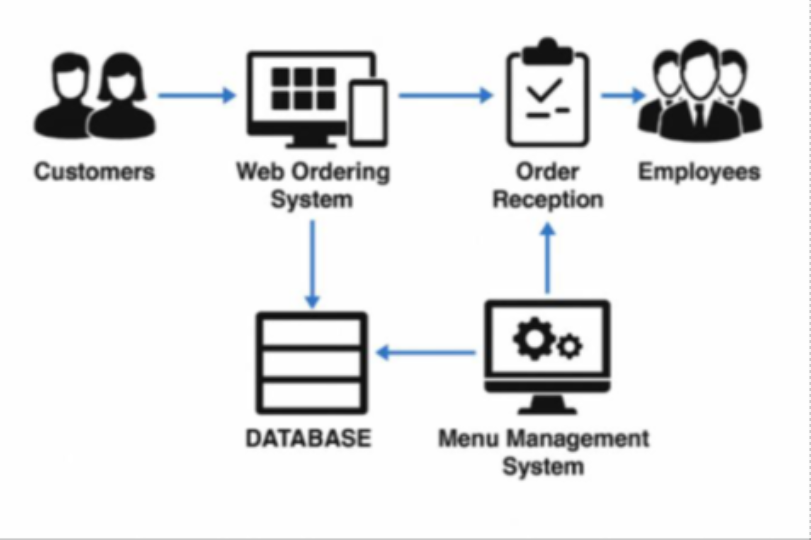
\includegraphics[width=.8\textwidth]{cdt/images/Arquitectura_Nwekori-Ignatius}}
        \caption{Arquitectura del sistema de Nwekori e Ignatius \cite{nwekori2025design}.}
        \label{fig:arquitecturaNwekoriIgnatius}
    \end{center}
\end{figure}


%=========================================================
% DONE
% !TeX root = proyecto.tex

%=========================================================
\chapter{ANÁLISIS DEL SISTEMA}
Este capítulo detalla el proceso analítico y metodológico seguido para transformar las necesidades detectadas en las cafeterías de la ESCOM en una solución de software estructurada. Se fundamenta en la captura de requisitos a través de la interacción directa con los operadores y el modelado sistemático del flujo de información. 

\section{METODOLOGÍA}
Para el desarrollo de este Trabajo Terminal se ha seleccionado el Modelo de Ciclo de Vida en Cascada (Waterfall). Esta elección se justifica por la necesidad de contar con una estructura secuencial y disciplinada que garantice que cada fase del diseño de ingeniería esté plenamente documentada antes de proceder a la construcción del software. 

El proceso se divide en las siguientes etapas: fase inicial donde se realizaron las entrevistas y observaciones directas para identificar las ineficiencias del modelo manual; análisis del sistema donde se registran los requerimientos funcionales y no funcionales, reglas de negocio y casos de uso; el diseño donde se contempla la arquitectura, el modelo entidad relación y el diseño de interfaces basado en las reglas de Shneiderman y Plaisant \cite{shneiderman2005designing}; la implementación; y las pruebas para evaluar el impacto del sistema. 

\subsection{RECOPILIACIÓN DE DATOS}
La fase de levantamiento de información se centró en una metodología de investigación cualitativa mediante entrevistas semiestructuradas. Estas fueron aplicadas a los encargados y personal de las cafeterías con el fin de obtener un diagnóstico profundo de la problemática operativa actual. Los entrevistados fueron cajeros y cocineros de las cafeterías Gamaretzi, In Kafen y Uni Café, concesionados actuales de los espacios dedicados para cafetería de las unidades académicas. 

\begingroup
\setlength{\LTleft}{\fill}
\setlength{\LTright}{\fill}

\begin{longtable}[c]{p{5cm} p{9cm}}
\caption{\textsc{Tabla de objetivos de las preguntas realizadas en entrevistas.}} \label{tab:objetivos-entrevistas} \\
\toprule
\textbf{Pregunta} & \textbf{Objetivo} \\
\midrule
\endfirsthead

\toprule
\textbf{Pregunta} & \textbf{Objetivo} \\
\midrule
\endhead

\midrule
\multicolumn{2}{r}{\small Continúa en la página siguiente...} \\
\endfoot
\bottomrule
\endlastfoot

¿Cómo gestionan actualmente la recepción de órdenes? (A papel, tickets, libretas)  & Identificar las fricciones en la comunicación verbal o por papel que provocan errores de preparación. \\
\addlinespace
¿Cómo gestionan los cambios en pedidos cuando ya están en proceso de preparación?  & Identificar fallas en la comunicación FoH-BoH. \\
\addlinespace
¿Cómo se le notifica a la cocina de este cambio? & Identificar las fricciones en la comunicación verbal o por papel que provocan errores de preparación. \\
\addlinespace
¿Cuáles son los principales errores al tomar un pedido? & Diagnosticar las ineficiencias de los sistemas manuales actuales en las cafeterías. \\
\addlinespace
¿Cómo afectan estos errores en el proceso de venta y preparación? & Evaluar el impacto en la fluidez operativa y la pérdida de ingresos. \\
\addlinespace
¿Cómo les indican a los clientes que ya está listo el pedido? & Modelar el flujo de notificaciones al usuario. \\
\addlinespace
¿Cómo deciden qué platillo cocinar primero? (¿Respetan el orden de llegada o por la facilidad de preparación?) & Establecer la línea base para la configuración del algoritmo MLFQ, detectando si el actual modelo FCFS es eficiente o genera bloqueos. \\
\addlinespace
¿Cuáles son los platillos que más tienden a atrasar la fila en horas pico y por qué? & Establecer la línea base para la configuración del algoritmo MLFQ, detectando si el actual modelo FCFS es eficiente o genera bloqueos. \\
\addlinespace
¿Cómo gestionan la cocina? ¿Por estaciones separadas? & Mapear la arquitectura física de producción para el enrutamiento de pedidos (plancha, barra fría, panes). \\
\addlinespace
¿En qué momento del proceso, sobre todo en horas pico, consideran que ``pierden el control'' de los pedidos? & Identificar el punto crítico donde la tasa de llegada supera la capacidad de servicio. \\
\addlinespace
¿Con qué frecuencia se quedan sin insumos para preparar los alimentos? & Fundamentar la necesidad de un módulo de gestión de inventarios con alertas críticas para evitar ventas de productos no disponibles \\
\addlinespace
¿Cómo gestionan esta falta de insumos y los pedidos que van llegando? & Justificar el módulo de gestión de inventarios con alertas críticas. \\
\addlinespace
¿Qué productos o ingredientes son más difíciles de mantener un conteo? & Fundamentar la necesidad de un módulo de gestión de inventarios con alertas críticas para evitar ventas de productos no disponibles \\
\addlinespace
En horas pico ¿Cuánto tiempo mínimo y máximo han notado que transcurre desde que el cliente hace una orden hasta que ustedes entregan el pedido? & Obtener datos para comparar el rendimiento actual contra los beneficios esperados de la digitalización \\
\addlinespace
En las mismas horas ¿Cuántos pedidos han llegado a acumularse? & Obtener datos para comparar el rendimiento actual contra los beneficios esperados de la digitalización \\
\addlinespace
¿Qué les facilitaría más el trabajo: saber qué pedidos vienen en los próximos 15 minutos o tener una pantalla que les organice los pedidos actuales por tipo de alimento? & Determinar si la prioridad del personal es el agrupamiento lógico (KDS) o la anticipación (pre-ordenamiento), lo que rige la jerarquía de información en las pantallas \\
\addlinespace
¿Qué tan fácil consideran que sería la integración de pantallas o pantallas táctiles mientras trabajan? & Validar la viabilidad del hardware (pantallas no táctiles) y del módulo de pre-ordenamiento para los estudiantes \\
\addlinespace
¿Han considerado o ya implementado un sistema de pedidos programados o por adelantado? & Validar la viabilidad del hardware (pantallas no táctiles) y del módulo de pre-ordenamiento para los estudiantes \\
\addlinespace
¿Cuál es la tarea que más les quita tiempo y que no tiene nada que ver con cocinar? & Identificar tareas administrativas para su automatización. \\
\end{longtable}
\endgroup

Con estas herramientas, entonces, se procederá al análisis del sistema.

\section{AGENTES DEL SISTEMA}
A partir de las entrevistas y la información estudiada, se han diagnosticado 5 agentes en el sistema. El primero corresponde al mánager, quien gestionar los productos y promociones disponibles, al personal y las reglas de cada cafetería. El segundo es el personal de la estación de caja, encargados de realizar los pedidos y cortes de caja e inventario. El siguiente corresponde al personal de cocina, quienes se dedican a la elaboración de los alimentos y apoyan en la gestión y el corte de inventario. Seguido de estos está el cliente, quien indica a caja los pedidos y consulta el menú. Finalmente se consideró un agente descentralizado de entrega quien, de acuerdo con lo diagnosticado, puede ser personal de cocina o personal de caja quienes entregan los alimentos y rotan según la demanda de actividades que corresponda a cada uno. Es con esto, entonces, que se procede con el análisis de requerimientos funcionales.

\section{REQUERIMIENTOS FUNCIONALES}

\subsection{MÓDULO DEL MANAGER}

\subsubsection{REQ-MGR-001: AUTENTICACIÓN DEL MÁNAGER}
El requerimiento REQ-MGR-001 precargado posee una prioridad Alta y está asignado al actor mánager. Se establece que el sistema debe ejecutar la autenticación del usuario mediante la validación estricta de sus credenciales y la confirmación del rol mánager antes de emitir cualquier token de sesión; de forma paralela, se debe efectuar el registro del evento en la entidad HistorialDeMovimientos. El criterio de aceptación determina que, ante la ausencia de una sesión activa, cuando el usuario ingresa credenciales válidas con dicho rol, se genera el token de sesión, se registra el evento INICIO\_SESION y se redirige al usuario a la interfaz MGR-02. Este componente se justifica debido a que la autenticación segura del módulo constituye una precondición obligatoria para el despliegue de todas las operaciones administrativas del sistema.

\subsubsection{REQ-MGR-002: DASHBOARD DE ALERTAS CRÍTICAS DE INVENTARIO}
El requerimiento REQ-MGR-002 precargado está catalogado con prioridad Alta para el actor mánager. Funcionalmente, el sistema debe desplegar en la interfaz del administrador la relación completa de aquellos productos que no se encuentran disponibles debido a la insuficiencia de insumos, así como detallar los insumos específicos que están en un nivel igual o inferior al umbral de alerta definido como parámetro. El criterio de aceptación estipula que, al acceder a la interfaz MGR-02, si al menos un insumo registra una variable cantidad\_stock menor o igual a umbral\_alerta, el tablero debe desplegar dinámicamente el componente visual del producto afectado y la fila correspondiente al insumo comprometido. Su desarrollo se justifica en la necesidad de proveer visibilidad en tiempo real respecto a los cuellos de botella operativos, optimizando la toma de decisiones orientadas al reabastecimiento. 

\subsubsection{REQ-MGR-003: GESTIÓN DEL DIRECTORIO DE PERSONAL}
El requerimiento REQ-MGR-003 precargado se define con una prioridad Media para el actor mánager. El sistema debe desplegar un directorio integral de los empleados, los cuales deben aparecer agrupados por su puesto jerárquico y con sus respectivas asignaciones de estaciones de trabajo, habilitando además la ejecución de búsquedas filtradas por los atributos de nombre, rol y estación. El criterio de aceptación requiere que, al acceder a la interfaz MGR-03 e ingresar un término de búsqueda, los componentes visuales se filtren automáticamente por coincidencia en los campos descritos. Se justifica bajo la premisa donde la organización del personal es indispensable para la supervisión operativa y el control de acceso lógico a las estaciones. 

\subsubsection{REQ-MGR-004: ALTA Y EDICIÓN DE EMPLEADOS CON ONBOARDING}
El requerimiento REQ-MGR-004 precargado se establece con prioridad Alta bajo la responsabilidad del actor mánager. La plataforma debe procesar el registro de nuevos empleados y accionar de manera automatizada un correo electrónico de onboarding orientado a la configuración inicial de la contraseña, permitiendo además la actualización posterior de datos y asignaciones. Como criterio de aceptación, cuando el administrador almacena un nuevo registro con datos válidos y una dirección de correo electrónico única, la entidad Empleado debe crearse bajo el estado PENDIENTE\_CONTRASENA y gestionar el correo electrónico de forma inmediata. La justificación técnica indica que este proceso automatizado mitiga errores de configuración inicial y garantiza el establecimiento de credenciales individuales preoperativas.

\subsubsection{REQ-MGR-005: RESTRICCIÓN DE TIPO ÚNICO DE ESTACIÓN POR EMPLEADO}
El requerimiento REQ-MGR-005 precargado posee prioridad Alta para el actor mánager. El sistema debe restringir la asociación de estaciones de modo que un empleado asignado a una estación de tipo COCINA solo pueda añadir estaciones de ese mismo tipo, aplicando restricción para el tipo CAJA. El criterio de aceptación es que, si un empleado posee una asignación activa a una estación de tipo COCINA, cualquier intento de asociar una estación de tipo CAJA debe ser bloqueado por el sistema, emitiendo un error explícito de incompatibilidad de tipos. Este control se justifica en la delegación de responsabilidades, la cual previene accesos cruzados no autorizados entre los módulos operativos. 

\subsubsection{REQ-MGR-006: DEFINICIÓN DE RECETA CON PASOS Y DEPENDENCIAS}
El requerimiento REQ-MGR-006 precargado cuenta con prioridad Alta para el actor mánager. Se concede la definición estructural de la receta de un producto mediante pasos secuenciales con dependencias de precedencia, especificación de ingredientes por paso y la asignación de la estación responsable. El criterio de aceptación exige que, al almacenar la receta, se persistan de forma atómica las entidades PasoReceta, IngredientePaso, EstacionPaso y DependenciaPaso, manteniendo el control de guardado deshabilitado en la interfaz hasta que la sumatoria de las cantidades distribuidas iguale con exactitud al total declarado. Su justificación radica en que esta estructura de pasos y dependencias alimenta directamente al Sistema de Despliegue de Cocina (KDS) y rige el flujo de producción.

\subsubsection{REQ-MGR-007: GESTIÓN DE PROMOCIONES Y COMBOS}
El requerimiento REQ-MGR-007 precargado se cataloga con prioridad Alta para el actor mánager. El sistema debe permitir la creación, modificación y eliminación de promociones y combos comerciales, especificando su composición, precio, recurso gráfico y ventana de vigencia temporal; los componentes adquieren un estado de inmutabilidad una vez que han sido transaccionados. El criterio de aceptación define que, cuando se almacena una promoción que incluye al menos un producto, si el atributo es\_temporal es verdadero y las fechas son válidas, la promoción debe ser visible exclusivamente dentro del rango definido. Se justifica para asegurar la correcta parametrización de las estrategias comerciales, previniendo discrepancias de precios y vigencias operativas. 

\subsubsection{REQ-MGR-008: CONFIGURACIÓN DE INGREDIENTES EXTRAS PARA MÓDULO CLIENTE}
El requerimiento REQ-MGR-008 precargado posee prioridad Alta para el actor mánager. El sistema debe permitir habilitar insumos específicos para ser ofertados como ingredientes extras en el módulo del cliente, determinando un costo adicional por unidad, listando únicamente aquellos insumos que tengan activos los atributos correspondientes. El criterio de aceptación dictamina que, cuando se activa el atributo ofrecer\_como\_extra con un precio mayor a cero, al momento en que un cliente accede al detalle de un producto, el insumo debe desplegarse en la sección de Extras de la interfaz CLI-07 con su respectivo cargo financiero. Se justifica debido a que faculta la monetización de personalización de productos y sincroniza el catálogo con la política de precios de la organización.

\subsection{REQ-MGR-010: CONFIGURACIÓN DEL SISTEMA}
El requerimiento REQ-MGR-010 precargado se define con prioridad Alta para el actor mánager. El sistema debe centralizar la configuración de parámetros globales, incluyendo el umbral de alerta de inventario, los métodos de pago autorizados, los cargos por empaque, las ventanas de recolección, los horarios de operación, las políticas de penalización y la estructura de turnos. El criterio de aceptación establece que, una vez que el administrador almacena las modificaciones en la interfaz MGR-27 con parámetros válidos, todos los módulos dependientes deben reflejar los nuevos valores de forma inmediata en la subsecuente consulta de datos. La justificación técnica reside en que la centralización paramétrica garantiza la coherencia operativa y la uniformidad de las reglas de negocio entre los módulos.

\subsubsection{REQ-MGR-011: GESTIÓN DE CREDENCIALES DE ESTACIONES}
El requerimiento REQ-MGR-011 precargado posee una prioridad Alta bajo el actor mánager. Se debe permitir la creación y administración de las credenciales compartidas correspondientes a las estaciones de tipo CAJA y ENTREGA, empleadas para la autenticación de las sesiones de terminal. El criterio de aceptación exige que, cuando se genera una credencial de tipo CAJA y el operador ingresa dichas credenciales, se establezca la sesión con el perfil CAJERO; si el tipo de credencial no coincide con el módulo receptor, la sesión debe ser rechazada de forma obligatoria. Su justificación estipula que las credenciales de estación habilitan la distribución de dispositivos físicos entre múltiples operadores sin daño en la trazabilidad por terminal.

\subsection{MÓDULO DE COCINA}

\subsubsection{REQ-COC-001: AUTENTICACIÓN INDIVIDUAL DEL COCINERO}
El requerimiento REQ-COC-001 precargado cuenta con prioridad Alta para el actor Cocinero. El sistema debe autenticar al personal de cocina mediante credenciales individuales, validando la existencia de al menos una entidad AsignacionEstacion activa cuyo tipo sea igual a COCINA; se estipula que las asignaciones de tipo TEMPORAL deben expirar automáticamente a las 23:59:59 del día en curso. El criterio de aceptación define que, cuando el empleado ingresa credenciales válidas con una estación de cocina activa, se procesa el acceso generando un token con el perfil COCINERO; si las asignaciones temporales han expirado, el acceso debe ser denegado. Se justifica para garantizar la trazabilidad individual de las operaciones en cocina y soportar la gestión de turnos con temporalidades dinámicas.

\subsubsection{REQ-COC-002: KDS PRINCIPAL CON TABLERO DE PASOS EN TIEMPO REAL}
El requerimiento REQ-COC-002 precargado se establece con prioridad Alta para el actor Cocinero. Se debe presentar en tiempo real un tablero reactivo con los pasos de preparación pendientes asociados a la estación activa, restringiendo la visualización a pasos en estado PENDIENTE cuyas tareas predecesoras cuenten de forma obligatoria con el estado COMPLETADO. El criterio de aceptación estipula que, cuando el cocinero selecciona una estación de trabajo, si un paso cumple con las condiciones de estado, estación y precedencia, la tarjeta correspondiente se despliega en el tablero; completar el paso actual cambia a su estado y libera el subsecuente. Se justifica en que rige la secuencia lógica de producción sin requerir de coordinación verbal o manual inter-estación.

\subsubsection{REQ-COC-003: ALGORITMO DE URGENCIA TEMPORAL POR PASO}
El requerimiento REQ-COC-003 precargado posee prioridad Alta para el actor Cocinero. El sistema debe calcular dinámicamente el índice de urgencia de cada paso de preparación. Al alcanzar o superar el umbral configurado, el estado debe mutar automáticamente a URGENTE, modificando los componentes visuales de la interfaz (borde, cronómetro y barra de progreso) de color negro a color rojo. El criterio de aceptación indica que, si un paso de producción se encuentra en estado PENDIENTE y la relación matemática iguala o supera el porcentaje\_urgencia, la interfaz debe cambiar visualmente a rojo de forma automatizada. Su justificación técnica es que actúa como un semáforo visual predictivo para priorizar la preparación de órdenes en riesgo de incumplir los tiempos de servicio.

\subsubsection{REQ-COC-004: LIBERACIÓN AUTOMÁTICA DE PASOS DEPENDIENTES}
El requerimiento REQ-COC-004 precargado se clasifica con prioridad Alta para el actor Cocinero. Al marcar un paso como COMPLETADO, el sistema debe evaluar de forma síncrona las dependencias asociadas de modo que, para todo paso subsiguiente cuyos predecesores se encuentren en su totalidad en estado COMPLETADO, se realice la transición automática de BLOQUEADO a PENDIENTE. El criterio de aceptación modela que, al ejecutar la acción de finalización sobre un paso P, cuando el sistema procesa la entidad DependenciaPasoPedido, los pasos dependientes que resulten viables deben cambiar a PENDIENTE y renderizarse en sus estaciones respectivas. Se justifica porque elimina los tiempos muertos de coordinación inter-estación, asegurando el cumplimiento estricto del diagrama de flujo de la receta.

\subsubsection{REQ-COC-005: FILTROS DE URGENCIA Y RESUMEN DE PEDIDOS EN KDS}
El requerimiento REQ-COC-005 precargado posee prioridad Media para el actor Cocinero. El sistema debe proveer filtros de visualización mutuamente excluyentes basados en el nivel de urgencia, disponiendo además de un contenedor lateral (drawer) de resumen que agrupe los pasos por producto y permita el resalto de tarjetas específicas. Como criterio de aceptación, si el cocinero activa el filtro de órdenes Urgentes, todas aquellas tarjetas con nivel\_urgencia igual a NO\_URGENTE deben disminuir su opacidad y bloquear su interactividad, manteniendo únicamente una visibilidad estática. Su desarrollo se justifica en que facilita la gestión de la carga cognitiva del personal en periodos de alta demanda mediante la discriminación visual de tareas.

\subsubsection{REQ-COC-006: SUB-ASIGNACIÓN DE PERSONAL POR COCINERO AUTORIZADO}
El requerimiento REQ-COC-006 precargado se define con prioridad Media para el actor Cocinero. Se faculta al personal de cocina que posea el atributo permite\_sub\_asignacion activo para acceder al panel de gestión con el fin de consultar y modificar las asignaciones de estaciones, salvaguardando la restricción de tipo único. El criterio de aceptación dictamina que, si un cocinero autorizado intenta modificar una asignación hacia una estación de tipo incompatible, el sistema debe bloquear el cambio; ante un flujo válido, debe registrar la bitácora ASOCIACION\_PERSONAL\_ESTACION. Se justifica debido a que descentraliza la administración del talento humano en la cocina, permitiendo adaptaciones dinámicas ante contingencias sin requerir escalamiento al mánager.

\subsubsection{REQ-COC-007: MODAL DE DETALLE COMPLETO DE RECETA DEL PEDIDO}
El requerimiento REQ-COC-007 precargado posee una prioridad Baja para el actor Cocinero. El sistema debe proveer una vista de solo lectura que detalle la totalidad de los pasos de la receta vinculada a un producto en un pedido activo, exponiendo de forma explícita el estado de completitud, los insumos requeridos, la estación destino y las dependencias estructurales. El criterio de aceptación establece que, cuando el cocinero interactúa con una tarjeta del KDS y el pedido asociado está en estado EN\_PREPARACION, se debe renderizar un modal estático con la información exacta del estado de la receta al momento del llamado. Su justificación es que facilita la comprensión global del proceso de elaboración, permitiendo al operario anticipar requerimientos técnicos logísticos de pasos futuros.

\subsubsection{REQ-COC-008: ENRUTAMIENTO POR ESTACIONES CON PASOS DE RECETA}
El requerimiento REQ-COC-008 precargado cuenta con prioridad Alta para el actor Cocinero. El sistema debe distribuir automáticamente los componentes de la receta de un pedido hacia las subestaciones configuradas por la administración; cada paso es direccionado en exclusividad al KDS correspondiente, y en caso de multi-asignación, se replica en los destinos. Como criterio de aceptación, si una tarea $P$ está indexada a las estaciones $E_1$ y $E_2$, al confirmarse el pedido, la tarea se despliega en ambos tableros, de modo que la ejecución del cierre en cualquiera de las estaciones marca el paso como COMPLETADO a nivel global. Se justifica porque automatiza la logística interna de producción, suprimiendo la necesidad de despachar órdenes o comandas físicas.  

\subsubsection{REQ-COC-009: DESCUENTO AUTOMÁTICO DE INVENTARIO POR RECETA AL CONFIRMAR PEDIDO}
El requerimiento REQ-COC-009 precargado se establece con prioridad Alta para el actor Cocinero. Al confirmarse el pago de un pedido en el punto de venta, el sistema debe ejecutar de forma automática el decremento proporcional de los insumos del inventario, basándose en la receta estándar y el factor de porción definido. El criterio de aceptación exige que, al confirmarse el pago de una orden en la interfaz CAJ-14, si el pedido comprende una cantidad N de un producto, el atributo stock\_actual decrezca de manera atómica. Su desarrollo se justifica en que garantiza la concordancia del inventario lógico con las existencias físicas en cocina, impidiendo desfases por procesamiento rezagado.

\subsection{MÓDULO DE ENTREGA}

\subsubsection{REQ-ENT-001: AUTENTICACIÓN DEL OPERADOR DE ENTREGA}
El requerimiento REQ-ENT-001 precargado posee prioridad Alta para el actor Operador de Entrega. El sistema debe autenticar al operador de despacho mediante las credenciales compartidas de la estación de tipo ENTREGA, vinculando la sesión al identificador id\_estacion y auditando el proceso bajo el concepto INICIO\_SESION en la entidad HistorialDeMovimientos. El criterio de aceptación define que, ante la ausencia de una sesión activa de entrega, cuando el operador ingresa credenciales válidas asignadas al tipo ENTREGA, se genera un token con perfil OPERADOR\_ENTREGA y se redirige a la interfaz ENT-02. Se justifica porque permite el uso multiusuario del dispositivo de despacho, resguardando la trazabilidad operativa por estación física.

\subsubsection{REQ-ENT-002: TABLERO PRINCIPAL DE PEDIDOS EN DESPACHO CON ESTADOS DIFERENCIADOS}
El requerimiento REQ-ENT-002 precargado se clasifica con prioridad Alta para el actor Operador de Entrega. Se debe presentar un tablero de control con los pedidos en estados activos (EN\_PREPARACION y PREPARADO), incorporando códigos cromáticos de urgencia calculados a partir del tiempo transcurrido frente al estimado o al límite de merma. El criterio de aceptación estipula que, en la interfaz ENT-02, si la relación de tiempo de preparación supera el porcentaje\_urgencia, la tarjeta muta de negro a rojo; si el tiempo en estado preparado excede el porcentaje\_merma, cambia de verde a amarillo. Su justificación técnica indica que mitiga la entrega de productos degradados (merma) y permite dar celeridad a los pedidos que presentan desviaciones en su tiempo de servicio.

\subsubsection{REQ-ENT-003: FILTROS DE PEDIDOS EN TABLERO DE DESPACHO}
El requerimiento REQ-ENT-003 precargado cuenta con prioridad Media para el actor Operador de Entrega. El sistema debe disponer de filtros de visualización mutuamente excluyentes basados en el estado (En proceso / Preparado), nivel de urgencia o modalidad de entrega; las tarjetas excluidas deben mitigar su presencia visual mediante atenuación y bloqueo operativo. Como criterio de aceptación, cuando el operador acciona el filtro de estado Preparado, todas aquellas tarjetas en estado EN\_PREPARACION deben disminuir su opacidad y restringir su interactividad hasta la desactivación del filtro. Se justifica debido a que optimiza la gestión visual del mostrador de despacho durante picos de alta afluencia de clientes.

\subsubsection{REQ-ENT-004: CANCELACIÓN DE ENTREGA CON MOTIVO NORMALIZADO}
El requerimiento REQ-ENT-004 precargado se define con prioridad Alta para el actor Operador de Entrega. El sistema debe facultar la cancelación de pedidos que se encuentren en estado EN\_PREPARACION o PREPARADO, exigiendo de forma obligatoria la selección de una causa indexada en la entidad MotivoCancelacionEntrega, siendo esta transacción de carácter irreversible. El criterio de aceptación establece que, al ejecutar la acción de cancelación y seleccionar un motivo válido de la lista, el atributo estado cambia a CANCELADO, se registra en HistorialDeMovimientos y la orden se remueve del tablero. Se justifica porque suministra datos estructurados para el análisis de mermas y proporciona sustento analítico ante eventuales reclamaciones de clientes.

\subsubsection{REQ-ENT-005: FLUJO DE PAGO Y VERIFICACIÓN DE DESPACHO CON ÁRBOL DE DECISIÓN}
El requerimiento REQ-ENT-005 precargado posee prioridad Alta para el actor Operador de Entrega. El sistema debe determinar dinámicamente la sub-vista del contenedor lateral de despacho basándose en el estado de cuenta de la orden y las directrices globales, prohibiendo de forma absoluta el avance a la validación QR si la orden registra saldo pendiente. El criterio de aceptación determina que, al abrir la interfaz ENT-04 de un pedido en estado PREPARADO y NO\_PAGADO, si el parámetro permite\_pago\_en\_entrega es verdadero y se procesa el cobro, el estado muta a PAGADO y se habilita el control de verificación. Su justificación establece que funciona como una compuerta lógica de control que impide la entrega material de productos no liquidados financieramente.

\subsubsection{REQ-ENT-006: GENERACIÓN Y VALIDACIÓN DE CÓDIGO QR DE IDENTIDAD DE UN SOLO USO}
El requerimiento REQ-ENT-006 precargado posee una prioridad Alta para el actor Operador de Entrega. El sistema debe generar un token criptográfico seguro (UUID v4) bajo el estado ACTIVO en la entidad CodigoVerificacionQR; el servidor validará el token mediante la verificación de vigencia, correspondencia de pedido, cliente y estado no consumido. Como criterio de aceptación, al invocar la interfaz ENT-05 para una orden apta, cuando el cliente presenta el QR y el servidor corrobora las cuatro condiciones de integridad, el estado del código muta a CONSUMIDO y la aplicación navega a la interfaz de éxito ENT-06. Su justificación radica en que el uso de tokens opacos y de un solo uso previene la suplantación de identidad y asegura la entrega legítima de la orden.

\subsubsection{REQ-ENT-007: CONFIRMACIÓN DE ENTREGA EXITOSA Y CIERRE DEL FLUJO}
El requerimiento REQ-ENT-007 precargado se cataloga con prioridad Alta para el actor Operador de Entrega. Al recibir una validación exitosa del código QR, el sistema debe cambiar el estado del pedido a ENTREGADO, estampar el atributo Timestamp\_entrega y registrar la bitácora ENTREGA\_PEDIDO de manera previa a la resolución de la interfaz de éxito. El criterio de aceptación modela que, tras recibir la confirmación síncrona de validación del QR y concluir la actualización de los atributos en el servidor, se renderiza la interfaz ENT-06; al cerrarse esta, la orden es removida definitivamente del tablero. Se justifica porque automatiza la finalización del flujo de despacho, disminuyendo las interacciones requeridas por el operador.

\subsubsection{REQ-ENT-008: GESTIÓN DE FALLO EN VERIFICACIÓN DE IDENTIDAD QR}
El requerimiento REQ-ENT-008 precargado cuenta con prioridad Alta para el actor Operador de Entrega. Ante una falla en la validación del código QR (token inválido, expirado o con inconsistencia de asignación), el sistema debe redirigir el flujo a la interfaz ENT-07 sin alterar el estado del pedido, revocando el token inválido para impedir reintentos. El criterio de aceptación estipula que, cuando el servidor dictamina una falla y la causa corresponde a token expirado, el estado de la entidad muta a EXPIRADO y se detallan las causales en la interfaz ENT-07, retornando posteriormente a ENT-04-C. Su justificación técnica indica que discrimina de forma precisa entre anomalías de carácter puramente técnico y posibles intentos de retiro fraudulento.

\subsubsection{REQ-ENT-009: VALIDAR CÓDIGO DE ENTREGA}
El requerimiento REQ-ENT-009 precargado posee prioridad Alta para el actor Operador de Entrega. El sistema debe permitir la captura manual del código alfanumérico de entrega provisto por el client para la validación de identidad y el despacho de la orden una vez que esta se encuentre en estado disponible para retiro. Como criterio de aceptación, si el operador ingresa el código de entrega en la interfaz de despacho y el valor coincide con el registro persistido estando la orden lista, el pedido se dictamina como entregado; de lo contrario, se mantiene el estado y se emite una alerta. Se justifica debido a que ofrece un mecanismo alterno de validación que salvaguarda la seguridad ante fallos en la lectura del componente gráfico QR.

\subsubsection{REQ-ENT-010: MARCAR PEDIDO COMO LISTO PARA RECOGER}
El requerimiento REQ-ENT-010 precargado se establece con prioridad Alta para el actor Cocinero. El sistema debe procesar de forma automatizada el cambio de estado de un pedido a listo para su retiro tras la culminación de sus tareas en cocina, desplegando un resumen de los ítems, el identificador numérico de la orden y el control de confirmación. El criterio de aceptación exige que, cuando el KDS registra el último paso como COMPLETADO y la totalidad de los pasos asociados a la orden alcanzan dicho estado, el atributo estado del pedido cambie automáticamente a PREPARADO y el tablero ENT-02 se actualice a color verde. Su justificación radica en que suprime las necesidades de comunicación verbal o interrupciones entre el área de producción y la zona de entrega.

\subsection{MÓDULO DE CAJA}

\subsubsection{REQ-CAJ-001: AUTENTICACIÓN DEL CAJERO CON CREDENCIALES DE ESTACIÓN}
El requerimiento REQ-CAJ-001 precargado cuenta con prioridad Alta para el actor Cajero. El sistema autentica al operador de caja mediante las credenciales compartidas de la estación de tipo CAJA configuradas por el Manager, quedando la sesión asociada al identificador de estación y registrando el evento en el historial de movimientos con concepto de inicio de sesión. El criterio de aceptación estipula que, ante la ausencia de una sesión activa en el dispositivo, cuando el operador ingresa credenciales válidas de una estación activa de tipo CAJA, el sistema genera un token de sesión con perfil CAJERO asociado al identificador de estación y redirige a la interfaz correspondiente; si las credenciales corresponden a una estación con tipo distinto, la sesión no se establece. Su justificación técnica indica que la autenticación por estación permite operar el módulo de Caja con credenciales compartidas manteniendo la trazabilidad de operaciones por dispositivo.

\subsubsection{REQ-CAJ-002: DASHBOARD DE ALERTAS OPERATIVAS DEL CAJERO}
El requerimiento REQ-CAJ-002 precargado cuenta con prioridad Alta para el actor Cajero. El sistema presenta las alertas operativas críticas del turno, incluyendo productos no disponibles por insuficiencia de insumos e insumos con existencias iguales o por debajo del umbral de alerta, proveyendo además acceso a nuevo pedido, inventario y cierre de sesión. El criterio de aceptación estipula que, cuando el cajero accede al dashboard y al menos un insumo tiene existencias iguales o inferiores al umbral de alerta, o un producto presenta stock insuficiente, el sistema despliega la tarjeta del producto no disponible y la fila del insumo en la tabla de estatus; el cierre de sesión registra el evento correspondiente en el historial de movimientos. Su justificación técnica indica que el cajero requiere visibilidad inmediata de productos no disponibles para evitar registrar pedidos que no pueden prepararse.

\subsubsection{REQ-CAJ-003: CATÁLOGO DE PRODUCTOS CON DISPONIBILIDAD EN TIEMPO REAL}
El requerimiento REQ-CAJ-003 precargado cuenta con prioridad Media para el actor Cajero. El sistema presenta el catálogo completo de productos con un indicador de disponibilidad calculado en tiempo real a partir del cruce de stock de insumos con las cantidades requeridas, permitiendo búsqueda por nombre, ingredientes y etiquetas, así como acceso al detalle de ingredientes y receta de cada producto. El criterio de aceptación dictamina que, cuando un insumo requerido no opcional de un producto tiene existencias inferiores a la cantidad requerida, dicho producto exhibe el indicador de no disponible, y que la búsqueda filtra por subcadena sobre nombre, ingredientes y etiquetas. Su justificación técnica indica que conocer el estado de disponibilidad del catálogo en tiempo real reduce errores al registrar pedidos de productos que no pueden elaborarse.

\subsubsection{REQ-CAJ-004: AJUSTE DE INVENTARIO CON TRAZABILIDAD DE CONCEPTO}
El requerimiento REQ-CAJ-004 precargado cuenta con prioridad Alta para el actor Cajero. El sistema permite registrar ajustes formales de stock sobre insumos individuales capturando la cantidad ajustada y el concepto justificativo del movimiento, normalizando el concepto en el catálogo correspondiente y registrando la operación en el historial de movimientos. El criterio de aceptación estipula que, cuando el cajero ingresa una cantidad distinta de cero y un concepto no vacío y confirma la operación, el sistema actualiza el stock del insumo y crea el registro en el historial con el concepto de ajuste de inventario; si el concepto no existe en el catálogo, se crea como nuevo registro. Su justificación técnica indica que la trazabilidad de ajustes con concepto permite auditar movimientos de stock y detectar discrepancias entre el estado físico y el sistema.

\subsubsection{REQ-CAJ-005: CREACIÓN DE PEDIDO CON CARRITO DE COMPRA MIXTO}
El requerimiento REQ-CAJ-005 precargado cuenta con prioridad Alta para el actor Cajero. El sistema permite construir un pedido seleccionando productos y promociones desde catálogos diferenciados, siendo el carrito un estado temporal de sesión no persistido; los productos que forman parte de una promoción activa se excluyen de la pestaña de productos individuales. El criterio de aceptación dictamina que, al seleccionar un producto o promoción disponible, el ítem se agrega al carrito temporal con precio base, y que el carrito permanece en sesión hasta la confirmación del pago o la cancelación explícita. Su justificación técnica indica que la separación entre productos individuales y combos protege la integridad del precio e impide duplicar descuentos de promoción.

\subsubsection{REQ-CAJ-006: PERSONALIZACIÓN DE INGREDIENTES POR ÍTEM DE PEDIDO}
El requerimiento REQ-CAJ-006 precargado cuenta con prioridad Alta para el actor Cajero. El sistema permite modificar la composición de ingredientes de un producto antes de agregarlo al carrito, habilitando la eliminación de ingredientes existentes, la adición de cualquier insumo del inventario como extra y el ajuste de cantidades, sin alterar las entidades maestras. El criterio de aceptación estipula que, al eliminar un ingrediente base o agregar un insumo extra, la configuración del ítem queda en sesión temporal con el indicador de variación activado, y que los extras con cargo adicional incrementan el costo del ítem sin que el descuento de stock ocurra en esta etapa. Su justificación técnica indica que la personalización de ingredientes en la caja soporta los requerimientos de clientes con restricciones alimentarias y maximiza la flexibilidad del servicio en mostrador.

\subsubsection{REQ-CAJ-007: RESUMEN DEL PEDIDO Y SELECCIÓN DE MÉTODO DE PAGO}
El requerimiento REQ-CAJ-007 precargado cuenta con prioridad Alta para el actor Cajero. El sistema presenta el resumen editable del pedido antes de confirmarlo, incluyendo ítems con cantidades y precios, subtotal, cargo por pedido para llevar cuando aplica, y un selector de método de pago limitado a los métodos habilitados en la configuración del sistema, con visibilidad del indicador de variación por ítem modificado. El criterio de aceptación dictamina que, al seleccionar un método de pago habilitado y confirmar, el sistema abre la interfaz de confirmación, calculando el cargo para llevar según la configuración del sistema y bloqueando los métodos no habilitados por el Manager. Su justificación técnica indica que el resumen previo a la confirmación reduce errores de cobro y asegura que el cajero y el cliente acuerden el monto total antes de ejecutar la transacción.

\subsubsection{REQ-CAJ-008: CONFIRMACIÓN DE PAGO Y ENCOLAMIENTO EN COCINA}
El requerimiento REQ-CAJ-008 precargado cuenta con prioridad Alta para el actor Cajero. El sistema solicita confirmación explícita de que el pago fue recibido y, al confirmar, persiste el pedido con estado de pago pagado, crea los registros de ítems como snapshot de precios y configuraciones, decrementa el stock de insumos y encola el pedido en el sistema de visualización de cocina. El criterio de aceptación estipula que, al confirmar el pago con un método seleccionado, el pedido cambia a estado pagado, se crean los snapshots de ítems, se decrementa el stock de cada ingrediente consumido y el pedido queda disponible en cocina, siendo esta operación irreversible desde la interfaz. Su justificación técnica indica que el snapshot de precios e ingredientes al momento del pago garantiza la integridad del historial ante cambios posteriores en el catálogo y protege al negocio ante disputas.

\subsubsection{REQ-CAJ-009: HISTORIAL DE PEDIDOS POR ESTACIÓN DE CAJA}
El requerimiento REQ-CAJ-009 precargado cuenta con prioridad Media para el actor Cajero. El sistema presenta el historial de pedidos originados desde la estación de caja activa, con capacidad de búsqueda por identificador de pedido, nombre de producto y nombre de promoción, permitiendo acceder al detalle individual y registrar pagos de pedidos pendientes. El criterio de aceptación dictamina que, al seleccionar un pedido con estado de pago no pagado y confirmar el registro, el sistema cambia el estado a pagado y registra el evento en el historial de movimientos, mostrando únicamente los pedidos de la estación activa en sesión. Su justificación técnica indica que el historial por estación permite gestionar cobros diferidos y mantiene la trazabilidad de las operaciones de cada punto de venta de forma independiente.

\subsubsection{REQ-CAJ-010: INCORPORACIÓN DE COMBOS AL PEDIDO SIN MODIFICACIÓN}
El requerimiento REQ-CAJ-010 precargado cuenta con prioridad Alta para el actor Cajero. El sistema permite agregar promociones y combos al carrito con selección de cantidad, siendo estas inmutables en su composición, por lo que el cajero no puede modificar los productos o ingredientes que conforman el combo durante el flujo de pedido. El criterio de aceptación estipula que, al seleccionar una promoción activa y confirmar la cantidad, el combo se agrega al carrito temporal a su precio definido, sin que el sistema permita modificar su composición desde esta interfaz. Su justificación técnica indica que la inmutabilidad de combos protege la integridad del precio y garantiza que las promociones se consuman exactamente como fueron definidas por el Manager.

\subsubsection{REQ-CAJ-011: REGISTRO DE PAGO CONTRA ENTREGA AL CREAR EL PEDIDO}
El requerimiento REQ-CAJ-011 precargado cuenta con prioridad Alta para el actor Cajero. El sistema permite registrar pagos al crear el pedido mediante el selector de método de pago, estando los métodos disponibles limitados a los habilitados por el Manager en la configuración del sistema. El criterio de aceptación estipula que, al seleccionar un método de pago y confirmar, el pedido queda registrado con el método seleccionado y el estado de pago pagado. Su justificación técnica indica que registrar el método de pago al crear el pedido permite al módulo de Entrega verificar el estado de cobro antes de despachar. 

\subsubsection{REQ-CAJ-012: PROGRAMACIÓN DE VENTANA DE RECOLECCIÓN PARA PEDIDO ANTICIPADO}
El requerimiento REQ-CAJ-012 precargado cuenta con prioridad Alta para el actor Cajero. El sistema presenta el modal de programación exclusivamente cuando el tipo de pedido es anticipado y el pago ha sido registrado exitosamente, permitiendo al operador seleccionar una ventana horaria de recolección entre las disponibles con capacidad calculada a partir de la configuración del sistema menos los pedidos activos en dicha ventana. Al confirmar, el sistema persiste la ventana de recolección y encola el pedido en el sistema de visualización de cocina. El criterio de aceptación dictamina que, al seleccionar una ventana con capacidad disponible y confirmar, la ventana queda asociada al pedido, el estado del pedido cambia a en preparación, el pedido se hace visible en cocina y la ocupación de la ventana se incrementa en uno; si el tipo de pedido es inmediato, el modal no se presenta y el flujo avanza directamente al ticket. Su justificación técnica indica que la programación explícita de ventana horaria permite distribuir la carga de preparación en cocina y garantizar al cliente un tiempo de entrega comprometido.

\subsubsection{REQ-CAJ-013: VALIDACIÓN DE CONCURRENCIA EN SELECCIÓN DE VENTANA DE ENTREGA PARA PEDIDO ANTICIPADO}
El requerimiento REQ-CAJ-013 precargado cuenta con prioridad Alta para el actor Cajero. El servidor revalida la capacidad disponible de la ventana seleccionada en el momento exacto de la confirmación, independientemente del valor mostrado al cargar el modal; si entre la visualización y la confirmación otro pedido ocupó el último espacio disponible, el servidor rechaza la operación sin modificar el estado del pedido y mantiene el modal activo para que el cajero seleccione una ventana alternativa. El criterio de aceptación estipula que, cuando un pedido concurrente ocupa el último espacio antes de que el cajero confirme, el servidor rechaza la operación con error de capacidad insuficiente, la ocupación de la ventana rechazada no se incrementa y el modal permanece abierto recalculando la lista de ventanas con la opción seleccionada marcada sin capacidad disponible. Su justificación técnica indica que la revalidación de capacidad al confirmar previene el sobrecupo de ventanas horarias cuando múltiples cajeros compiten simultáneamente por el último espacio disponible.

\subsection{MÓDULO DEL CLIENTE}

\subsubsection{RNFU-10 MANEJO DE PERMISOS DE CÁMARA PARA ESCANEO QR EN APLICACIÓN WEB}
El requerimiento RNFU-10 precargado se establece con prioridad Alta para el actor Cliente. La plataforma debe gestionar de forma controlada el ciclo de vida del permiso de acceso a la cámara periférica requerido para las funcionalidades de escaneo QR en CLI-14 y CLI-16, asegurando que, si el usuario revoca o deniega dicho acceso, se despliegue un mensaje de orientación técnica sin incurrir en excepciones no controladas ni interrupciones del entorno gráfico. El criterio de aceptación determina que, ante la denegación del permiso solicitado por el navegador, el sistema presente textualmente la notificación: ``Se requiere acceso a la cámara para escanear el código. Habilita el permiso en la configuración de tu navegador.'', manteniendo el botón de escaneo completamente operativo para futuros reintentos. Se justifica en que el tratamiento estructurado de la denegación de periféricos salvaguarda la resiliencia de la interfaz y faculta al usuario para corregir el estado de forma autónoma sin demandar soporte técnico externo.

\subsubsection{REQ-CLI-001: AUTENTICACIÓN INDIVIDUAL DEL CLIENTE}
El requerimiento REQ-CLI-001 precargado cuenta con prioridad Alta para el actor Cliente. El sistema autentica al cliente mediante credenciales individuales, distinguiendo entre credenciales inválidas y cuenta desactivada, y ofreciendo un enlace de recuperación de contraseña; a diferencia de los módulos Caja y Entrega, no utiliza credenciales de estación compartidas. El criterio de aceptación estipula que, al ingresar credenciales válidas con cuenta activa, se genera un token de sesión con perfil de cliente y se redirige al catálogo; si la cuenta está desactivada, el mensaje de error distingue este caso de las credenciales inválidas. Su justificación técnica indica que la autenticación individual protege el historial de pedidos y el código QR de recolección de accesos no autorizados.

\subsubsection{REQ-CLI-002: CATÁLOGO PRINCIPAL CON BANNER DE CAPACIDAD DISPONIBLE}
El requerimiento REQ-CLI-002 precargado cuenta con prioridad Alta para el actor Cliente. El sistema presenta el catálogo de la cafetería con un banner que muestra la capacidad disponible de la próxima ventana de recolección, calculada como la capacidad máxima menos el conteo de pedidos confirmados no cancelados, siendo los ítems sin stock suficiente no navegables. El criterio de aceptación dictamina que, cuando un insumo de un producto tiene stock insuficiente, la tarjeta muestra un indicador rojo sin navegación disponible, y que el banner refleja los espacios disponibles calculados en tiempo real. Su justificación técnica indica que el banner de capacidad orienta al cliente sobre la disponibilidad de espacios antes de iniciar su pedido, reduciendo la tasa de abandono por ventana llena al confirmar.

\subsubsection{REQ-CLI-003: BÚSQUEDA DE PRODUCTOS Y PROMOCIONES}
El requerimiento REQ-CLI-003 precargado cuenta con prioridad Media para el actor Cliente. El sistema ejecuta búsqueda de texto libre sobre el catálogo con comparación insensible a mayúsculas y coincidencia de subcadena, incluyendo en los resultados los ítems no disponibles con indicador rojo, pero sin navegación al detalle. El criterio de aceptación estipula que, al ingresar al menos un carácter en la barra de búsqueda, la lista se volverá a ejecutará al modificar el término mostrando resultados con los disponibles primero; de no existir coincidencias, el sistema despliega un mensaje informativo. Su justificación técnica indica que la búsqueda de texto libre mejora la conversión al permitir que el cliente localice rápidamente un ítem sin navegar todo el catálogo.

\subsubsection{REQ-CLI-004: SELECCIÓN DE EXTRAS OPCIONALES CON PRECIO DINÁMICO}
El requerimiento REQ-CLI-004 precargado cuenta con prioridad Alta para el actor Cliente. El sistema presenta los ingredientes extra opcionales de un producto con casilla de selección individual y control de cantidad por extra, recalculando el precio total en tiempo real como la suma del precio base más el costo de cada ingrediente adicional marcado y multiplicado por su cantidad. El criterio de aceptación dictamina que, al marcar un extra, se habilita el control de cantidad inicializado en uno y el precio total se actualiza en pantalla; al desmarcarlo, el extra se excluye del cálculo, y la configuración de extras seleccionados se almacena como snapshot en la sesión del carrito. Su justificación técnica indica que el precio dinámico permite al cliente conocer el costo exacto de su personalización antes de agregar el ítem al carrito.

\subsubsection{REQ-CLI-005: GESTIÓN DEL CARRITO DE COMPRAS DEL CLIENTE}
El requerimiento REQ-CLI-005 precargado cuenta con prioridad Alta para el actor Cliente. El sistema mantiene el estado del carrito en sesión local, permitiendo ajustar cantidades por ítem con eliminación automática al decrementar desde uno, eliminar ítems individuales y vaciar el carrito con confirmación explícita, recalculando el total de forma dinámica; la disponibilidad de ítems no se vuelve a verificar en el carrito, sino en el servidor al confirmar el pedido. El criterio de aceptación estipula que, al vaciar el carrito y confirmar, todos los ítems son eliminados de la sesión, el botón de proceder al pago permanece deshabilitado mientras no haya ítems, y el total refleja el precio unitario con extras multiplicado por la cantidad de cada ítem. Su justificación técnica indica que el carrito en sesión local permite al cliente revisar y ajustar su pedido antes de comprometer stock del inventario.

\subsubsection{REQ-CLI-006: ACEPTACIÓN DE POLÍTICA DE PAGO CONTRA ENTREGA}
El requerimiento REQ-CLI-006 precargado cuenta con prioridad Alta para el actor Cliente. El sistema requiere la aceptación explícita de la política de pago contra entrega mediante un botón de selección antes de proceder al paso de selección de horario, siendo el rechazo o la cancelación acciones que retornan al carrito sin persistir cambios en el servidor; la aceptación no genera un registro independiente, sino que se incorpora como atributo del pedido. El criterio de aceptación estipula que, al seleccionar la opción de aceptar, el botón de selección de recolección se habilita, mientras que al rechazar o cancelar, el cliente regresa al carrito sin cambios. Su justificación técnica indica que la aceptación explícita del esquema de pago contra entrega es un requisito legal y operativo que protege a la cafetería ante pedidos no recogidos.

\subsubsection{REQ-CLI-007: SELECCIÓN DE VENTANA DE RECOLECCIÓN CON VALIDACIÓN DE CONCURRENCIA}
El requerimiento REQ-CLI-007 precargado cuenta con prioridad Alta para el actor Cliente. El sistema presenta las ventanas de tiempo de recolección disponibles generadas a partir del horario de operación y el tamaño de ventana configurados en el sistema, siendo las ventanas sin capacidad y las anteriores a la hora actual no seleccionables; la capacidad no se reserva hasta la confirmación del pedido. El criterio de aceptación dictamina que, al seleccionar una ventana con capacidad disponible, esta queda asociada al estado local del flujo y que, si al confirmar la ventana ya no tiene capacidad, el servidor rechaza el pedido y redirige al cliente para una nueva selección. Su justificación técnica indica que la gestión de ventanas con validación en confirmación resuelve condiciones de carrera entre clientes concurrentes sin bloquear espacios prematuramente.

\subsubsection{REQ-CLI-008: CONFIRMACIÓN DE PEDIDO CON VALIDACIONES TRANSACCIONALES EN SERVIDOR}
El requerimiento REQ-CLI-008 precargado cuenta con prioridad Alta para el actor Cliente. Al confirmar el pedido, el servidor ejecuta en secuencia la verificación del carrito, la disponibilidad de stock por ítem, la capacidad de la ventana seleccionada y la vigencia de sesión; si todas las validaciones son exitosas, crea el registro del pedido en estado de preparación, genera los ítems como snapshot de precios vigentes, decrementa el stock de insumos e incrementa la ocupación de la ventana. El criterio de aceptación estipula que, al validar exitosamente stock y capacidad, el pedido se crea en estado de preparación, se generan los snapshots, se decrementa el stock y se limpia la sesión del carrito; si falla el stock, el ítem afectado se señala, y si falla la capacidad, redirige a la selección de ventana. Su justificación técnica indica que la atomicidad de las validaciones en la confirmación garantiza la integridad del pedido y previene la sobreventa de capacidad o productos sin stock.

\subsubsection{REQ-CLI-009: SEGUIMIENTO DE PEDIDOS PENDIENTES DE RECOLECCIÓN}
El requerimiento REQ-CLI-009 precargado cuenta con prioridad Alta para el actor Cliente. El sistema presenta la lista de pedidos activos del cliente con una barra de progreso que refleja el avance en cocina, actualizándose en tiempo real mediante mecanismo de notificación para reflejar cambios de estado propagados desde los módulos de Cocina y Entrega. El criterio de aceptación dictamina que, cuando al menos un pedido se encuentra en preparación o preparado, se muestra la lista con barra de progreso por pedido, siendo el botón de recolección accesible independientemente del estado, ya que la validación ocurre en el módulo de Entrega. Su justificación técnica indica que el seguimiento en tiempo real reduce la incertidumbre del cliente y disminuye las consultas al personal de mostrador.

\subsubsection{REQ-CLI-010: VERIFICACIÓN DE IDENTIDAD QR PARA RECOLECCIÓN}
El requerimiento REQ-CLI-010 precargado cuenta con prioridad Alta para el actor Cliente. El sistema permite al cliente abrir el lector de QR mediante la API de cámara del navegador y enviar el token escaneado al endpoint de verificación, siendo el token de un solo uso de modo que un reintento con el mismo produce error de token ya consumido. El criterio de aceptación estipula que, al escanear el QR y validar el servidor el token, el identificador del pedido y el del cliente, el pedido cambia a estado entregado, el código de verificación se marca como consumido y el botón de escaneo se deshabilita; si la validación falla, se muestra un mensaje de error y el botón permanece activo para reintento con nuevo código. Su justificación técnica indica que el protocolo QR de un solo uso garantiza que solo el cliente propietario del pedido pueda completar la recolección, previniendo entregas fraudulentas.

\subsubsection{REQ-CLI-011: GESTIÓN DEL PERFIL DEL CLIENTE}
El requerimiento REQ-CLI-011 precargado cuenta con prioridad Media para el actor Cliente. El sistema permite al cliente autenticado actualizar sus datos personales mediante operación sobre la entidad correspondiente, verificando el servidor la unicidad del correo antes de persistir y calculando el hash de contraseña en servidor; el campo de contraseña se presenta vacío al cargar y, si se deja vacío, la contraseña no se modifica. El criterio de aceptación estipula que, al intentar modificar el correo a uno ya registrado, el servidor rechaza el cambio con un mensaje de correo en uso, y que si la nueva contraseña tiene menos de ocho caracteres el servidor la rechaza; los cambios no guardados se descartan al navegar fuera sin confirmación adicional. Su justificación técnica indica que la gestión del perfil es una funcionalidad de autoservicio que reduce la carga de soporte al permitir al cliente actualizar sus datos de contacto sin intervención del Manager.

\subsubsection{REQ-CLI-012: ORQUESTACIÓN DE MENÚ BASADA EN DISPONIBILIDAD REAL DE INSUMOS}
El requerimiento REQ-CLI-012 precargado cuenta con prioridad Alta para el actor Cliente. El sistema sincroniza la disponibilidad del catálogo con el estado real del inventario, marcando automáticamente como no disponible cualquier producto cuyo insumo crítico tenga stock insuficiente para al menos una porción, reflejando el indicador correspondiente en todas las vistas del catálogo. El criterio de aceptación dictamina que, cuando el stock de un insumo resulta insuficiente para al menos una porción de un producto dependiente, todos los módulos del sistema reflejan dicho producto como no disponible en su próxima consulta al servidor. Su justificación técnica indica que la sincronización automática de disponibilidad previene que el cliente genere pedidos de productos que no pueden elaborarse por falta de ingredientes.

\subsubsection{REQ-CLI-013: GESTIÓN DINÁMICA DE VENTANAS DE TIEMPO}
El requerimiento REQ-CLI-013 precargado cuenta con prioridad Alta para el actor Cliente. El sistema ofrece una selección de intervalos de tiempo para la recolección del pedido, calculados dinámicamente dividiendo el horario de operación en bloques del tamaño configurado y evaluando la ocupación actual de cada bloque. El criterio de aceptación estipula que, al generar los intervalos del día, solo se muestran como seleccionables aquellos con hora de inicio posterior a la hora actual y con capacidad disponible, mientras que los intervalos llenos se renderizan con tratamiento visual diferenciado y sin acción de selección. Su justificación técnica indica que las ventanas dinámicas permiten distribuir la carga de pedidos a lo largo del día evitando saturación simultánea en cocina.

\subsubsection{REQ-CLI-014: GENERACIÓN DE CÓDIGO DE ENTREGA QR}
El requerimiento REQ-CLI-014 precargado cuenta con prioridad Alta para el actor Cliente. El sistema permite al cliente iniciar el proceso de verificación de identidad escaneando el código QR generado por el módulo de Entrega, codificando dicho código únicamente un token opaco de un solo uso sin datos del pedido embebidos. El criterio de aceptación dictamina que, al activar el lector de QR y escanear el código, el token es enviado al servidor para validación y el resultado se recibe de forma asíncrona, sin que el código generado contenga identificadores de pedido ni datos sensibles. Su justificación técnica indica que el código QR de un solo uso es el mecanismo de verificación de identidad que protege la integridad de la entrega y asegura que el pedido llegue al cliente correcto. 

\subsection{REQ-CLI-015: NOTIFICACIONES Y SEGUIMIENTO DE ESTADO DEL PEDIDO}
El requerimiento REQ-CLI-015 precargado cuenta con prioridad Alta para el actor Cliente. El sistema informa al cliente sobre el progreso de su pedido mediante una barra de progreso que refleja los estados de preparación y listo, propagando en tiempo real los cambios de estado desde los módulos de Cocina y Entrega. El criterio de aceptación estipula que, cuando el módulo de Cocina marca el último paso de un pedido como completado y el pedido cambia a estado preparado, la barra de progreso alcanza el cien por ciento y el botón de recolección permanece accesible, sin que el cliente requiera recargar la página para ver el cambio. Su justificación técnica indica que informar al cliente en tiempo real sobre el estado de su pedido reduce su tiempo de espera en mostrador y mejora la experiencia de servicio.

\subsubsection{REQ-CLI-016: ACCESO ANÓNIMO A RESUMEN DE PEDIDO MEDIANTE TOKEN DE URL}
El requerimiento REQ-CLI-016 precargado cuenta con prioridad Alta para el actor Cliente. El sistema permite a un usuario no autenticado consultar el resumen completo de un pedido generado en el módulo Caja accediendo mediante una URL con token, exponiendo la barra de progreso, número de pedido, fecha y hora de creación, tiempo transcurrido, contenido como snapshot de ítems, horario de entrega, método de pago y total; el acceso se deniega cuando el pedido tiene un cliente asociado, sin transmitir ningún dato al solicitante. El criterio de aceptación dictamina que, al acceder con un token válido y un pedido sin cliente asociado, el servidor retorna el resumen completo sin requerir autenticación; si el pedido tiene cliente asociado, el servidor retorna error de acceso denegado sin incluir datos del pedido en la respuesta. Su justificación técnica indica que el acceso anónimo al resumen permite a clientes sin cuenta registrada realizar seguimiento de su pedido y ejecutar el protocolo de recolección mediante QR sin requerir la creación de una cuenta en el sistema.

\subsubsection{REQ-CLI-017: CONTROL DE ACCESO DIFERENCIADO POR ASOCIACIÓN DEL PEDIDO A CUENTA DE CLIENTE}
El requerimiento REQ-CLI-017 precargado cuenta con prioridad Alta para el actor Cliente. El sistema diferencia el nivel de acceso al resumen del pedido según la asociación de este a una cuenta: si el pedido no tiene cliente asociado el acceso anónimo mediante token está permitido; si tiene cliente asociado el acceso anónimo es denegado sin transmitir dato alguno al solicitante, siendo el cliente autenticado propietario quien accede mediante su sesión activa. El criterio de aceptación estipula que, al presentar un token válido para un pedido con cliente asociado, el servidor devuelve error de acceso denegado sin incluir ningún campo del pedido en la respuesta, mientras que el token de resumen permanece inaccesible para el usuario anónimo, pero no es invalidado. Su justificación técnica indica que el control de acceso diferenciado protege la privacidad de los pedidos asociados a cuentas registradas e impide que terceros con acceso al token consulten información de clientes autenticados.

\subsubsection{REQ-CLI-018: VERIFICACIÓN QR DE ENTREGA DESDE INTERFAZ DE ACCESO ANÓNIMO}
El requerimiento REQ-CLI-018 precargado cuenta con prioridad Alta para el actor Cliente. El sistema permite al usuario anónimo iniciar el protocolo de verificación de entrega activando el lector de QR mediante la API de cámara del navegador, enviando el token decodificado al endpoint de verificación del módulo de Entrega y recibiendo el resultado de forma asíncrona; en caso de éxito el pedido cambia a estado entregado, el código de verificación se marca como consumido y el botón queda deshabilitado, mientras que en caso de fallo se muestra el error descriptivo y el botón permanece activo para reintento. El criterio de aceptación dictamina que, al escanear un token válido y no consumido con el pedido en estado disponible para su recolección, el servidor valida el token, modifica el estado del pedido a entregado y el código a consumido, y la interfaz recibe el resultado y deshabilita el botón; si el token es inválido, expirado o ya consumido, el servidor retorna error sin modificar el estado del pedido. Su justificación técnica indica que la capacidad de verificar la entrega desde la interfaz anónima cierra el ciclo de vida del pedido para clientes sin cuenta registrada sin requerir intervención de módulos adicionales ni registro previo en el sistema.

\subsection{REQUERIMIENTOS GLOBALES}
\subsubsection{REQ-GLB-001: ACTUALIZACIÓN EN TIEMPO REAL ENTRE MÓDULOS MEDIANTE PUSH}
El requerimiento REQ-GLB-001 precargado se establece con prioridad Alta para el actor Global. El sistema debe implementar una arquitectura de comunicación bidireccional en tiempo real (mediante WebSockets o Server-Sent Events) para enlazar los módulos Cocina, Entrega y Cliente, propagando cambios de estado sin requerir la recarga manual de páginas. Como criterio de aceptación, cuando el área de cocina finaliza el último paso de una orden y todas las entidades PasoPedidoEstado se registran en estado COMPLETADO, el servidor distribuye el estado PREPARADO a los tableros ENT-02 y CLI-13 simultáneamente. Su justificación técnica indica que sincroniza el ecosistema de software para actuar como una plataforma unificada y reactiva en lugar de operar como silos de información independientes.

\subsubsection{REQ-GLB-002: MODELO DE PAGO EXCLUSIVAMENTE CONTRA ENTREGA EN MÓDULO CLIENTE}
El requerimiento REQ-GLB-002 precargado posee prioridad Alta para el actor Global. El módulo orientado al cliente debe operar bajo la restricción de un esquema financiero exclusivo de pago contra entrega, omitiendo de forma total la integración de pasarelas de pago digitales en las interfaces desde CLI-01 hasta CLI-15. El criterio de aceptación exige que, al ejecutar la confirmación de una orden en la interfaz CLI-11 y persistirse el registro en el servidor, el atributo metodo\_pago adopte de forma fija la modalidad contra entrega, omitiendo campos bancarios en el frontend. Se justifica en que el aislamiento de este modelo de pago reduce la complejidad del desarrollo, elimina costos de intermediación y mitiga riesgos de fraude electrónico.

\subsubsection{REQ-GLB-003: SNAPSHOT DE PRECIOS E INGREDIENTES EN CONFIRMACIÓN DE PEDIDO}
El requerimiento REQ-GLB-003 precargado cuenta con prioridad Alta para el actor Global. En el instante en que se confirma una orden (procedente de Caja o Cliente), el sistema debe almacenar los precios vigentes y las configuraciones de insumos como un registro histórico inmutable en la entidad ItemPedido, garantizando que mutaciones posteriores en el catálogo no alteren los datos pasados. El criterio de aceptación establece que, si la administración modifica el precio de un bien posterior a la confirmación de una orden, al auditar el historial de transacciones de dicho pedido, el valor desplegado debe acogerse estrictamente al atributo precio\_unitario\_snapshot. Su desarrollo se justifica para resguardar la consistencia y salud de las auditorías contables, protegiendo al establecimiento ante discrepancias de precios.

\subsubsection{REQ-GLB-004: BITÁCORA CENTRALIZADA DE MOVIMIENTOS DEL SISTEMA}
El requerimiento REQ-GLB-004 precargado se define con prioridad Alta para el actor Global. El sistema debe registrar de manera automatizada en la entidad HistorialDeMovimientos las transacciones críticas del entorno: INICIO\_SESION, CIERRE\_SESION, AJUSTE\_INVENTARIO, ASOCIACION\_PERSONAL\_ESTACION, CANCELACION\_ENTREGA, ENTREGA\_PEDIDO y REGISTRO\_PAGO\_ENTREGA. Como criterio de aceptación, cuando un componente ejecuta una operación sujeta a trazabilidad y el servidor procesa la transacción, se debe escribir de forma paralela en la bitácora el concepto descriptivo, el identificador del operador y la marca temporal. Se justifica debido a que la bitácora centralizada constituye el instrumento primordial de auditoría informática para la detección de irregularidades operativas.

\subsubsection{REQ-GLB-005: VERIFICACIÓN DE SESIÓN ACTIVA COMO PRECONDICIÓN DE INTERFAZ}
El requerimiento REQ-GLB-005 precargado posee prioridad Alta para el actor Global. En la totalidad de los módulos constituyentes, la posesión de una sesión activa con el perfil idóneo se establece como una precondición obligatoria para la interacción con las interfaces de usuario, validando el token de sesión en cada petición HTTP. El criterio de aceptación dictamina que, si un token de sesión expira o es revocado, cuando el cliente remite una solicitud a cualquier recurso protegido del servidor, el backend deniega el acceso mediante un código de error y fuerza la redirección a la pantalla de login. Su justificación técnica radica en que previene el acceso lógico no autorizado a funciones críticas del sistema ante escenarios de tokens comprometidos o terminales abandonadas.

\subsubsection{REQ-GLB-006: GESTIÓN DE DISPONIBILIDAD DE PRODUCTOS POR STOCK DE INSUMOS}
El requerimiento REQ-GLB-006 precargado se establece con prioridad Alta para el actor Global. El sistema debe dictaminar la disponibilidad de los productos evaluando en el servidor si las existencias actuales de cada insumo obligatorio cubren la cantidad de porción configurada; el cálculo debe mantener consistencia global en cada carga de catálogo. El criterio de aceptación determina que, si el nivel de existencias de un insumo cae por debajo del requerimiento de una receta, ante la invocación de la lectura del catálogo en cualquier módulo, el artículo debe computarse y desplegarse simultáneamente bajo el estado de No disponible. Se justifica bajo la premisa de que la centralización de las reglas de negocio del inventario asegura la consistencia de la información expuesta a los usuarios en todos los puntos de contacto del sistema.

\section{REQUERIMIENTOS NO FUNCIONALES}
\subsection{REQUERIMIENTOS GLOBALES}
\subsubsection{RNFU-01 ACCESO BASADO EN ROLES}
El requerimiento RNFU-01 precargado se establece con prioridad Alta para el actor Global. Este comprende la implementación de un mecanismo de control de acceso basado en roles con el propósito de restringir las funciones de la plataforma de acuerdo con el perfil del usuario, abarcando explícitamente las clasificaciones de Administrador, Cocina, Caja y Cliente. El criterio de aceptación determina que el sistema exija de manera obligatoria credenciales de autenticación para permitir el ingreso a las funcionalidades restringidas, que las contraseñas se almacenen mediante algoritmos de cifrado en la base de datos y que únicamente los usuarios validados puedan interactuar con la interfaz. Se justifica bajo la premisa de que esta restricción salvaguarda la confidencialidad de la información y evita accesos no autorizados a operaciones y datos sensibles.

\subsubsection{RNFU-02 INTEGRIDAD DE LOS PEDIDOS}
El requerimiento RNFU-02 precargado se establece con prioridad Alta para el actor Global. El sistema debe garantizar que no se generen registros duplicados de transacciones de pedidos dentro de la base de datos. El criterio de aceptación estipula que la plataforma incorpore controles de validación robustos que impidan la inserción repetida de una misma orden; ante un intento de duplicación, el proceso debe ser bloqueado de forma automática o, en su defecto, notificar al usuario a través de un mensaje informativo estructurado. Se justifica en que la mitigación de registros redundantes es imperativa para mantener una gestión fidedigna de las órdenes y prevenir fallos logísticos durante la preparación o la entrega física de productos.

\subsubsection{RNFU-03 PERSISTENCIA DE LA INFORMACIÓN}
El requerimiento RNFU-03 precargado se establece con prioridad Alta para el actor Global. Se estipula que, una vez confirmado un pedido por parte del usuario, el sistema garantice la persistencia de la información y evite la pérdida de datos ante la presencia de fallos parciales o caídas de la plataforma. El criterio de aceptación determina que las órdenes debidamente confirmadas permanezcan almacenadas de forma permanente en la base de datos y puedan recuperarse íntegramente tras un reinicio de la aplicación o una restauración de la operación general del servidor. Se justifica debido a que la preservación de los pedidos es esencial para asegurar la continuidad del servicio y mitigar inconsistencias operativas en el entorno de trabajo.

\subsubsection{RNFU-04 CONSISTENCIA EN TRANSACCIONES}
El requerimiento RNFU-04 precargado se establece con prioridad Alta para el actor Global. Las operaciones vinculadas con el registro y la actualización de los pedidos deben ejecutarse bajo los principios de atomicidad y consistencia para salvaguardar la integridad de la base de datos. El criterio de aceptación determina que dichas operaciones se ejecuten de manera completa o se cancelen en su totalidad ante la presencia de un error en el flujo, garantizando que la base de datos conserve un estado consistente y predecible tras cada transacción. Se justifica en que la consistencia de los datos asegura que los procesos del sistema no den lugar a estados incongruentes o corruptos en la información almacenada.

\subsubsection{RNFU-05 ESCALABILIDAD DEL SISTEMA}
El requerimiento RNFU-05 precargado se establece con prioridad Alta para el actor Global. La arquitectura de software del sistema debe permitir la integración de múltiples cafeterías concurrentes dentro de la misma infraestructura tecnológica corporativa. El criterio de aceptación determina que la plataforma permita registrar y gestionar la información operativa correspondiente a distintas sedes o cafeterías, manteniendo los datos asociados a cada una de ellas separados lógicamente e identificados. Se justifica en que este atributo de calidad viabiliza la expansión futura del sistema para atender diferentes puntos de venta sin la necesidad de rediseñar integralmente la solución de software base.

\subsubsection{RNFU-06 SEGURIDAD DE TOKENS DE ACCESO ANÓNIMO MEDIANTE IDENTIFICADORES OPACOS}
El requerimiento RNFU-06 precargado se establece con prioridad Alta para el actor Global. El sistema debe generar tokens de acceso anónimo orientados a la visualización de resúmenes de pedidos (PedidoAccesoAnonimo.token) utilizando identificadores UUID v4 o equivalentes criptográficamente opacos, garantizando que no se exponga el identificador numérico Pedido.id ni datos sensibles asociados; el servidor resolverá internamente dicha relación sin transmitirla al cliente, y cualquier intento de acceso con valores secuenciales o arbitrarios en la URL devolverá un estado HTTP 404 sin revelar la existencia real del recurso. El criterio de aceptación determina que, cuando un usuario intente acceder a la interfaz CLI-16 mediante un token, el servidor procese la petición y entregue los datos omitiendo el Pedido.id secuencial en la respuesta; de igual manera, ante un token inválido o manipulado, se debe retornar un error HTTP 404. Se justifica bajo el principio de que la opacidad del token impide ataques de enumeración de recursos, evitando que actores maliciosos accedan a información de terceros mediante la iteración de la URL.

\subsubsection{RNFU-07 CICLO DE VIDA DE TOKENS QR DE VERIFICACIÓN DE ENTREGA DE UN SOLO USO}
El requerimiento RNFU-07 precargado se establece con prioridad Alta para el actor Global. El sistema debe garantizar que cada identificador CodigoVerificacionQR.token sea válido únicamente para una sola operación de validación exitosa, transicionando inmediatamente al estado CONSUMIDO para que cualquier intento posterior sea rechazado de forma definitiva sin alterar el estado del pedido, mientras que los tokens no utilizados durante el periodo operacional transicionarán al estado EXPIRADO. El criterio de aceptación determina que, tras el consumo exitoso del token en la acción ENT-05, cualquier intento de revalidación por los módulos CLI-14, CLI-16 o ENT-05 devuelva un mensaje de error explícito indicando la invalidez del token por consumo previo, manteniendo inalterado el Pedido.estado. Se justifica en que la naturaleza efímera y de uso único del token QR imposibilita que la captura no autorizada de la imagen permita reclamar fraudulentamente un pedido que ya ha sido despachado.

\subsubsection{RNFU-08 TIEMPO DE RESPUESTA MÁXIMO EN OPERACIONES TRANSACCIONES DE CAJA}
El requerimiento RNFU-08 precargado se establece con prioridad Alta para el actor Global. El servidor debe completar y retornar la respuesta para transacciones críticas, tales como la confirmación de pago en CAJ-14, la asignación de ventanas horarias en CAJ-26 y la confirmación de pedidos en CLI-11, en un tiempo límite de 2 segundos bajo condiciones normales de operación local (on-premise), extendiéndose a un máximo de 3 segundos para operaciones de lectura; si este umbral es superado, el sistema desplegará un indicador visual de carga y suspenderá los reintentos automáticos para mitigar la duplicidad de transacciones. El criterio de aceptación estipula que, dentro del horario de operación en red local, el procesamiento y respuesta de las acciones en CAJ-26 o CLI-11 se efectúen en un intervalo menor o igual a 2 segundos, mientras que la carga del catálogo se complete en un tiempo menor o igual a 3 segundos. Se justifica debido a que la baja latencia en el punto de venta representa una necesidad operativa crítica, pues reduce los tiempos de espera y optimiza la capacidad de atención en periodos de alta demanda dentro de la cafetería universitaria.

\subsubsection{RNFU-11 CONTROL DE CONDICIÓN DE CARRERA EN ASIGNACIÓN DE CAPACIDAD POR VENTANA HORARIA}
El requerimiento RNFU-11 precargado se establece con prioridad Alta para el actor Global. El sistema debe ejecutar una validación de capacidad en el servidor de manera síncrona al momento de la confirmación de la ventana horaria, tanto en el flujo de caja (CAJ-26) como en el de cliente (CLI-10 / CLI-11), garantizando que dos peticiones concurrentes que compitan por la última plaza disponible resulten exactamente en una aprobación y una denegación, impidiendo que la ocupación total exceda el parámetro ConfiguracionSistema.capacidad\_maxima\_ventana. El criterio de aceptación determina que, ante el arribo simultáneo de dos solicitudes de reserva, una de ellas sea aceptada con éxito y la otra reciba un código de error por capacidad insuficiente, asegurando que la expresión COUNT(Pedido WHERE ventana = slot AND estado NOT IN ('CANCELADO')) permanezca siempre por debajo o igual al límite configurado. Se justifica en que el control estricto de las condiciones de carrera evita el sobrecupo operacional en la cocina, protegiendo la calidad del servicio y garantizando el cumplimiento de los tiempos de entrega comprometidos.

\subsection{MÓDULO DEL CLIENTE}
\subsubsection{RNFUN-13 ADAPTABILIDAD DE LA INTERFAZ}
El requerimiento RNFUN-13 precargado se establece con prioridad Alta para el actor Cliente. La interfaz gráfica de usuario debe poseer propiedades de adaptabilidad frente a diversas resoluciones y arquitecturas de hardware, facilitando su correcta renderización y operabilidad en entornos multiplataforma. El criterio de aceptación estipula que los componentes visuales del sistema mantengan una distribución armónica, accesible y funcional independientemente de las dimensiones de la pantalla del dispositivo utilizado. Se justifica bajo la premisa de que un diseño responsivo optimiza de forma transversal la experiencia del usuario final sin restringir los canales de acceso tecnológicos.

\subsection{MÓDULO DEL MÁNAGER}
\subsubsection{RNFU-07 GESTIÓN DE ROLES}
El requerimiento RNFU-07 precargado se establece con prioridad Alta para el actor mánager. El sistema debe incorporar un esquema estructurado de control de acceso basado en roles que discrimine con precisión los privilegios y las vistas operativas correspondientes a cada tipología de usuario. El criterio de aceptación determina que cada entidad de usuario posea un rol unívoco dentro de la persistencia de datos, de modo que las funcionalidades del sistema se habiliten o restrinjan de manera automatizada según dicha asignación. Se justifica bajo la necesidad de descentralizar y gobernar las operaciones del sistema, garantizando la restricción estricta de acciones con base en las responsabilidades del perfil institucional.

\subsubsection{RNFU-08 RESTRICCIÓN DE CONFIGURACIONES CRÍTICAS}
El requerimiento RNFU-08 precargado se establece con prioridad Alta para el actor mánager. Se determina que cualquier modificación relacionada con los niveles de inventario, configuraciones globales del sistema o parámetros operativos críticos quede restringida de forma exclusiva a los usuarios que posean el rol de administrador. El criterio de aceptación establece que solo los perfiles administrativos estén autorizados para invocar las interfaces y servicios de modificación crítica, bloqueando dichos privilegios al resto de los actores de la plataforma. Se justifica en que el aislamiento de las configuraciones del núcleo previene alteraciones accidentales o maliciosas que pongan en riesgo la continuidad de la operación comercial.

\subsubsection{RNFU-09 REGISTRO DE ACTIVIDADES}
El requerimiento RNFU-09 precargado se establece con prioridad Alta para el actor mánager. El sistema debe integrar un mecanismo persistente de bitácora de auditoría encargado de registrar cronológicamente los eventos significativos y las transacciones críticas ejecutadas por los usuarios. El criterio de aceptación estipula que las acciones relevantes se almacenen en un repositorio histórico inmutable que faculte la posterior consulta y trazabilidad de las operaciones efectuadas en la plataforma. Se justifica debido a que disponer de un registro detallado de actividades es indispensable para auditar el comportamiento del sistema, diagnosticar fallos técnicos y mantener la rendición de cuentas operativa.

\subsection{MÓDULO DE COCINA}
\subsubsection{RNFUN-10 OPERACIÓN CON CONECTIVIDAD LIMITADA}
El requerimiento RNFUN-10 precargado se establece con prioridad Alta para el actor Cocinero. El módulo orientado a la cocina debe asegurar la persistencia visual y la consulta de los pedidos previamente sincronizados bajo escenarios de degradación de red o conectividad intermitente. El criterio de aceptación determina que las órdenes registradas sigan expuestas en la interfaz de usuario de forma ininterrumpida hasta que ocurra una mutación de su estado o se marquen explícitamente como concluidas por el personal. Se justifica en que la disponibilidad constante de la cola de producción previene la paralización de las actividades del personal y resguarda la integridad de los datos frente a contingencias de infraestructura local.

\subsubsection{RNFUN-11 INTERACCIÓN MEDIANTE DIPOSITIVOS TÁCTILES}
El requerimiento RNFUN-11 precargado se establece con prioridad Alta para el actor Cocinero. La interfaz gráfica del módulo de cocina debe estar optimizada para interactuar mediante pantallas táctiles o periféricos de control simplificados acordes al entorno industrial de trabajo. El criterio de aceptación establece que los elementos de control en pantalla respondan con precisión a eventos táctiles y que la navegación resulte intuitiva y ágil para el operario. Se justifica bajo la premisa de que las condiciones ambientales de un área de producción culinaria exigen interfaces dinámicas que reduzcan la fricción operativa y aceleren los tiempos de respuesta manual.

\subsubsection{RNFUN-12 LEGIBILIDAD EN EL ENTORNO DE TRABAJO}
El requerimiento RNFUN-12 precargado se establece con prioridad Alta para el actor Cocinero. Se exige que el diseño visual del entorno de cocina garantice un contraste y tamaño tipográfico óptimos que aseguren la legibilidad remota de la información bajo las condiciones lumínicas del área de trabajo. El criterio de aceptación determina que los datos de los pedidos e insumos puedan ser reconocidos e interpretados sin ambigüedades por el personal durante el transcurso de la jornada. Se justifica en que una legibilidad adecuada disminuye drásticamente los errores humanos de interpretación en las comandas, optimizando el flujo de preparación.

\subsection{MÓDULO DE CAJA}
\subsubsection{RUSA-01: USABILIDAD EN EL REGISTRO DE PEDIDOS}
El requerimiento RUSA-01 precargado cuenta con prioridad Alta para el actor Cajero. La interfaz del módulo de caja debe estar diseñada para permitir el registro de pedidos de manera clara, intuitiva y eficiente para el operador. El criterio de aceptación estipula que el operador de caja puede registrar pedidos mediante los controles disponibles en la interfaz, seleccionando productos y confirmando pedidos de forma clara. Su justificación técnica indica que una interfaz sencilla facilita la operación del sistema por parte del personal de caja y reduce errores durante el registro de pedidos.

\subsection{MÓDULO DEL CLIENTE}
%% TODO

\newpage
\begin{landscape}
\section{REGLAS DE NEGOCIO}
\subsection{MÓDULO DEL MÁNAGER}
\subsubsection{AUTENTICACIÓN Y CONTROL DE SESIÓN}

\begingroup
\setlength{\LTleft}{\fill}
\setlength{\LTright}{\fill}

\begin{longtable}[c]{l p{2.1cm} p{2.1cm} p{8cm} p{4cm} c}
\caption{\textsc{Reglas de negocio del módulo del mánager para autenticación y control de sesión.}} \label{tab:reglas-negocio-manager-sesion} \\
\toprule
\textbf{ID} & \textbf{Título} & \textbf{Taxonomía} & \textbf{Descripción Anatómica} & \textbf{Entidades Acopladas} & \textbf{Interfaz Origen} \\
\midrule
\endfirsthead

\toprule
\textbf{ID} & \textbf{Título} & \textbf{Taxonomía} & \textbf{Descripción Anatómica} & \textbf{Entidades Acopladas} & \textbf{Interfaz Origen} \\
\midrule
\endhead

\midrule
\multicolumn{6}{r}{\small Continúa en la página siguiente...} \\
\endfoot
\bottomrule
\endlastfoot

RN-MGR-001 & Verificación de rol mánager en autenticación & [Control de Acceso] & El sistema emite un token de sesión con perfil mánager única y exclusivamente cuando las credenciales provistas corresponden a un registro Usuario con rol = mánager y estado activo. Si el registro existe, pero el rol difiere, la autenticación es rechazada. & Usuario (id, correo, hash\_contrasena, rol) & MGR-01 \\
\addlinespace
RN-MGR-002 & Registro obligatorio de inicio de sesión en bitácora & [Restricción Operacional] & Toda autenticación exitosa del perfil mánager genera de forma síncrona un registro en HistorialDeMovimientos con concepto INICIO\_SESION y el identificador del usuario autenticado como responsable. El fallo de este registro invalida la sesión. & HistorialDeMovimientos (concepto, id\_responsable, fecha) & MGR-01 \\
\addlinespace
RN-MGR-003 & Invalidación de sesión con registro en bitácora & [Restricción Operacional] & La acción de cierre de sesión invalida el token activo del mánager y genera de forma síncrona un registro en HistorialDeMovimientos con concepto CIERRE\_SESION antes de redirigir al login. & HistorialDeMovimientos & MGR-02 \\
\addlinespace
RN-MGR-024 & Invalidación de sesión activa al cambiar contraseña del mánager & [Restricción Operacional] & El cambio de contraseña del mánager en MGR-28 es aceptado únicamente si la contraseña actual provista coincide con Usuario.hash\_contrasena. Tras persistir la nueva contraseña, el sistema invalida el token de sesión activo del mánager e inicia un nuevo proceso de autenticación. Comportamiento estándar de seguridad para prevenir el uso de sesiones activas comprometidas tras cambio de credenciales. & Usuario (hash\_contrasena), token de sesión & MGR-28 \\
\end{longtable}
\endgroup

\subsubsection{GESTIÓN DE ALERTAS E INVENTARIO}
\begingroup
\setlength{\LTleft}{\fill}
\setlength{\LTright}{\fill}

\begin{longtable}[c]{l p{2.1cm} p{2.1cm} p{8cm} p{4cm} c}
\caption{\textsc{Reglas de negocio del módulo del mánager para gestión de alerta e inventario.}} \label{tab:reglas-negocio-manager-alertas}\\
\toprule
\textbf{ID} & \textbf{Título} & \textbf{Taxonomía} & \textbf{Descripción Anatómica} & \textbf{Entidades Acopladas} & \textbf{Interfaz Origen} \\
\midrule
\endfirsthead

\toprule
\textbf{ID} & \textbf{Título} & \textbf{Taxonomía} & \textbf{Descripción Anatómica} & \textbf{Entidades Acopladas} & \textbf{Interfaz Origen} \\
\midrule
\endhead

\midrule
\multicolumn{6}{r}{\small Continúa en la página siguiente...} \\
\endfoot
\bottomrule
\endlastfoot

RN-MGR-004 & Cálculo de disponibilidad de producto por stock & [Derivación / Algorítmica] & El sistema clasifica un producto como no disponible cuando existe al menos un insumo con es\_opcional = false en la relación IngredienteProducto cuya Insumo.cantidad\_stock $<$ IngredienteProducto.cantidad\_requerida. La evaluación se realiza individualmente para cada producto sobre el inventario en tiempo real. & Producto, IngredienteProducto, Insumo (cantidad\_stock, cantidad\_requerida, es\_opcional) & MGR-02, MGR-06 \\
\addlinespace
RN-MGR-005 & Umbral de alerta de insumo configurable por registro & [Derivación / Algorítmica] & Un insumo se incluye en el panel de alertas cuando su cantidad\_stock $\le$ umbral\_alerta. El campo umbral\_alerta es configurable individualmente por registro de insumo en MGR-16. El umbral global de ConfiguracionSistema opera como valor predeterminado cuando el umbral individual no está definido. & Insumo (cantidad\_stock, umbral\_alerta), ConfiguracionSistema (umbral\_alerta\_global) & MGR-02, MGR-16 \\
\addlinespace
RN-MGR-006 & Los insumos opcionales no bloquean la disponibilidad del producto & [Restricción Operacional] & Los insumos vinculados a un producto con IngredienteProducto.es\_opcional = true no participan en el cálculo de disponibilidad del producto. Un producto se considera disponible, aunque todos sus insumos opcionales tengan stock = 0, siempre que los insumos con es\_opcional = false sean suficientes. & IngredienteProducto (es\_opcional), Insumo & MGR-02, MGR-07 \\
\end{longtable}
\endgroup

\subsubsection{GESTIÓN DE PERSONAL Y ESTACIONES}
\begingroup
\setlength{\LTleft}{\fill}
\setlength{\LTright}{\fill}

\begin{longtable}[c]{l p{2.1cm} p{2.1cm} p{8cm} p{4cm} p{3cm}}
\caption{\textsc{Reglas de negocio del módulo del mánager para gestión de personal y de estaciones.}} \label{tab:reglas-negocio-manager-personal}\\
\toprule
\textbf{ID} & \textbf{Título} & \textbf{Taxonomía} & \textbf{Descripción Anatómica} & \textbf{Entidades Acopladas} & \textbf{Interfaz Origen} \\
\midrule
\endfirsthead

\toprule
\textbf{ID} & \textbf{Título} & \textbf{Taxonomía} & \textbf{Descripción Anatómica} & \textbf{Entidades Acopladas} & \textbf{Interfaz Origen} \\
\midrule
\endhead

\midrule
\multicolumn{6}{r}{\small Continúa en la página siguiente...} \\
\endfoot
\bottomrule
\endlastfoot

RN-MGR-007 & Unicidad de tipo de estación por empleado & [Restricción Operacional] & Una vez que un empleado tiene al menos una AsignacionEstacion con estación de tipo COCINA, el sistema rechaza toda nueva asociación con estaciones de tipo CAJA para ese empleado, y viceversa. Esta restricción aplica con independencia del rol del actor que realiza la asignación (Manager o cocinero con permiso de sub-asignación). & AsignacionEstacion (id\_empleado, id\_estacion), Estacion (tipo) & MGR-04, MGR-05 \\
\addlinespace
RN-MGR-008 & Expiración automática de asignaciones temporales a las 23:59:59 & [Derivación / Algorítmica] & Las asignaciones de tipo TEMPORAL expiran a las 23:59:59 del día calendario en que se crean. A partir de ese instante, el sistema no considera esa asignación como activa en ningún proceso de validación de acceso o autorización. & AsignacionEstacion (tipo\_temporalidad, fecha\_inicio, fecha\_fin) & MGR-04 \\
\addlinespace
RN-MGR-009 & Estado PENDIENTE\_CONTRASENA al crear empleado & [Validación Estructural] & Todo nuevo registro de Empleado es creado con estado PENDIENTE\_CONTRASENA. El estado no cambia a ACTIVO hasta que el empleado completa el flujo de establecimiento de contraseña mediante el enlace de onboarding de único uso enviado al correo registrado. & Empleado (estado) & MGR-04 \\
\addlinespace
RN-MGR-010 & Unicidad de correo electrónico de empleado & [Validación Estructural] & El campo Empleado.correo debe ser único en el sistema. El servidor rechaza el alta o edición de un empleado cuando el correo provisto ya existe en otro registro activo de la entidad Empleado. & Empleado (correo) & MGR-04 \\
\addlinespace
RN-MGR-011 & Alcance del permiso de sub-asignación & [Control de Acceso] & El permiso Empleado.permite\_sub\_asignacion = true habilita al empleado para acceder a la interfaz de gestión de personal de su módulo operativo y modificar asignaciones de estaciones de otros empleados. El tipo de temporalidad que puede asignar está limitado al conjunto habilitado en Empleado.tipo\_sub\_asignacion. No puede exceder los permisos definidos para él por el mánager. & Empleado (permite\_sub\_asignacion, tipo\_sub\_asignacion) & MGR-04 \\
\addlinespace
RN-MGR-012 & Alta de empleados restringida al perfil mánager & [Control de Acceso] & La creación de nuevos registros de empleados (INSERT en la entidad Empleado) es una operación exclusiva del perfil mánager. Los usuarios con perfil COCINERO con permiso de sub-asignación pueden modificar asignaciones de estaciones, pero no pueden crear, eliminar ni modificar los atributos de identidad de un empleado. & Empleado & MGR-03, MGR-04, COC-03 \\
\addlinespace
RN-MGR-030 & Modelo de autenticación diferenciado e incompatible por tipo de estación & [Control de Acceso] & Las estaciones de tipo ENTREGA operan exclusivamente mediante credenciales compartidas almacenadas en CredencialEstacion y no tienen personal asignado nominalmente en AsignacionEstacion. Las estaciones de tipo COCINA y CAJA son autenticadas mediante credenciales individuales de Empleado y no poseen registro en CredencialEstacion. Los dos modelos de autenticación son mutuamente excluyentes por tipo de estación. & Estacion (tipo), CredencialEstacion, AsignacionEstacion, Empleado & MGR-29, MGR-30-A, MGR-30-B \\
\addlinespace
RN-MGR-031 & Eliminación de estación bloqueada por dependencias activas en recetas & [Restricción Operacional] & El sistema rechaza la eliminación de una estación cuando existen registros en EstacionPaso que la referencian como estación asignada a pasos de receta vigentes, o cuando existen registros en PasoPedidoEstado con estado IN (PENDIENTE, BLOQUEADO) asignados a esa estación. La eliminación solo procede cuando la estación no tiene dependencias activas en ninguna entidad que la referencie. & Estacion, EstacionPaso, PasoPedidoEstado & MGR-30-A \\
\addlinespace
RN-MGR-032 & Etiquetas de estación como criterio de filtrado en asignación de pasos de receta & [Derivación / Algorítmica] & Las etiquetas (EtiquetaEstacion) asociadas a una estación de tipo COCINA actúan como atributos de clasificación utilizados como criterio de filtrado en la interfaz de asignación de estaciones a pasos de receta (MGR-13). El mánager puede filtrar el catálogo de estaciones disponibles por etiquetas para localizar estaciones specializadas según el tipo de preparación de cada paso. Las etiquetas no restringen la asignación; son únicamente un mecanismo de filtrado de catálogo. & EtiquetaEstacion, Etiqueta, EstacionPaso & MGR-30-A \\
\addlinespace
RN-MGR-033 & Credenciales de estación no replicadas en operación de duplicado & [Restricción Operacional] & Al duplicar una estación de tipo ENTREGA, el sistema genera el nuevo registro de Estacion sin incluir ni copiar el registro de CredencialEstacion de la estación origen. Las credenciales de la nueva estación deben ser definidas explícitamente por el mánager antes de que el acceso a la estación sea posible. La reutilización de credenciales entre estaciones distintas violaría el principio de trazabilidad de sesión por estación; cada estación debe tener credenciales únicas. & Estacion, CredencialEstacion & MGR-30-B \\
\addlinespace
RN-MGR-034 & Actualización de credenciales de estación como operación atómica independiente & [Restricción Operacional] & El sistema permite actualizar los campos de CredencialEstacion (usuario y hash\_contrasena) de una estación de tipo ENTREGA de forma atómica e independiente de la modificación de los demás atributos de la estación (nombre, tipo). La operación de actualización de credenciales se persiste sin requerir que el formulario completo esté en estado de guardado. & CredencialEstacion (usuario, hash\_contrasena) & MGR-30-B \\
\end{longtable}
\endgroup

\subsubsection{GESTIÓN DE PRODUCTOS Y RECETAS}
\begingroup
\setlength{\LTleft}{\fill}
\setlength{\LTright}{\fill}

\begin{longtable}[c]{l p{2.1cm} p{2.1cm} p{8cm} p{4cm} p{3cm}}
\caption{\textsc{Reglas de negocio del módulo del mánager para gestión de productos y de recetas.}} \label{tab:reglas-negocio-manager-recetas}\\
\toprule
\textbf{ID} & \textbf{Título} & \textbf{Taxonomía} & \textbf{Descripción Anatómica} & \textbf{Entidades Acopladas} & \textbf{Interfaz Origen} \\
\midrule
\endfirsthead

\toprule
\textbf{ID} & \textbf{Título} & \textbf{Taxonomía} & \textbf{Descripción Anatómica} & \textbf{Entidades Acopladas} & \textbf{Interfaz Origen} \\
\midrule
\endhead

\midrule
\multicolumn{6}{r}{\small Continúa en la página siguiente...} \\
\endfoot
\bottomrule
\endlastfoot

RN-MGR-013 & Invariante de distribución completa de ingredientes en receta & [Validación Estructural] & El sistema inhabilita la transición de estado a GUARDADO de un producto mientras la suma de cantidades de cada ingrediente distribuida en los pasos de la receta no sea exactamente igual a la cantidad total declarada para ese ingrediente en la ficha maestra del producto. La condición se evalúa por ingrediente de forma independiente. Formalmente:$\forall$ ingrediente\_i: SUM(IngredientePaso.cantidad WHERE id\_insumo = i) = IngredienteProducto.cantidad WHERE id\_insumo = i. & IngredienteProducto (cantidad), IngredientePaso (id\_paso, id\_insumo, cantidad) & MGR-08, MGR-11 \\
\addlinespace
RN-MGR-014 & Ingredientes opcionales como personalizaciones del módulo Cliente & [Control de Acceso] & Solo los ingredientes de un producto con IngredienteProducto.es\_opcional = true son presentados como opciones de personalización al cliente en el módulo Cliente (CLI-07). El módulo Caja puede agregar como extra cualquier insumo del inventario sin restricción de opcionalidad. & IngredienteProducto (es\_opcional) & MGR-08 \\
\addlinespace
RN-MGR-015 & Los insumos desechables no cuentan en el contador de distribución de receta & [Restricción Operacional] & Los insumos asociados a un producto con categoría DESECHABLE son gestionados en la entidad InsumoDesechableProducto y no afectan el contador de ingredientes pendientes de distribución en la pestaña ``Receta''. El invariante de distribución completa (RN-MGR-013) aplica únicamente sobre ingredientes con categoría INGREDIENTE. & InsumoDesechableProducto, IngredienteProducto, Insumo (categoria) & MGR-08 \\
\addlinespace
RN-MGR-016 & Preservación de dependencias al reordenar pasos & [Restricción Operacional] & Cuando el mánager reordena los pasos de una receta mediante arrastre, el sistema evalúa si algún paso predecesor declarado en DependenciaPaso quedaría posicionado después de su paso dependiente. En caso afirmativo, el sistema relocaliza automáticamente los predecesores a la posición inmediatamente anterior al paso dependiente para preservar la integridad de la cadena de dependencias. & PasoReceta (orden), DependenciaPaso (id\_paso, id\_paso\_predecesor) & MGR-11 \\
\addlinespace
RN-MGR-017 & Prohibición de auto-referencia en dependencias de pasos & [Validación Estructural] & El sistema rechaza el registro de una DependenciaPaso donde id\_paso = id\_paso\_predecesor. No se admite que un paso se declare predecesor de sí mismo. El sistema debe adicionalmente validar ausencia de dependencias circulares (e.g. A→B, B→A) que generarían deadlocks en el KDS. La detección de ciclos sobre un DAG (Directed Acyclic Graph) debe ejecutarse al persistir cualquier nueva relación de dependencia. & DependenciaPaso (id\_paso, id\_paso\_predecesor) & MGR-13 \\
\addlinespace
RN-MGR-018 & Cargo por extra activo solo en ingredientes opcionales & [Restricción Operacional] & El campo IngredienteProducto.precio\_extra solo es habilitado para captura y persistencia cuando IngredienteProducto.es\_opcional = true. Para ingredientes no opcionales, el campo permanece en estado nulo y no se transfiere al cálculo del precio del ítem en ningún módulo. & IngredienteProducto (es\_opcional, precio\_extra) & MGR-08 \\
\end{longtable}
\endgroup

\subsubsection{GESTIÓN DE PROMOCIONES}
\begingroup
\setlength{\LTleft}{\fill}
\setlength{\LTright}{\fill}

\begin{longtable}[c]{l p{2.1cm} p{2.1cm} p{8cm} p{4cm} p{3cm}}
\caption{\textsc{Reglas de negocio del módulo del mánager para gestión de promociones.}} \label{tab:reglas-negocio-manager-promociones}\\
\toprule
\textbf{ID} & \textbf{Título} & \textbf{Taxonomía} & \textbf{Descripción Anatómica} & \textbf{Entidades Acopladas} & \textbf{Interfaz Origen} \\
\midrule
\endfirsthead

\toprule
\textbf{ID} & \textbf{Título} & \textbf{Taxonomía} & \textbf{Descripción Anatómica} & \textbf{Entidades Acopladas} & \textbf{Interfaz Origen} \\
\midrule
\endhead

\midrule
\multicolumn{6}{r}{\small Continúa en la página siguiente...} \\
\endfoot
\bottomrule
\endlastfoot

RN-MGR-019 & Inmutabilidad de la composición de promoción en flujos de pedido & [Restricción Operacional] & Los productos que conforman una promoción (ProductoPromocion) no pueden ser modificados durante el flujo de creación de un pedido desde ningún módulo (Caja o Cliente). La promoción se oferta y se procesa como una unidad atómica e indivisible. La única variable configurable durante el pedido es la cantidad de unidades de la promoción a ordenar. & Promocion, ProductoPromocion & MGR-18, CAJ-15, CLI-04 \\
\addlinespace
RN-MGR-020 & Vigencia temporal automática de promoción & [Derivación / Algorítmica] & Una promoción con es\_temporal = true es visible y seleccionable en los módulos de pedido únicamente cuando fecha\_inicio $\le$ fecha\_actual $\le$ fecha\_fin. Fuera de ese rango, la promoción se clasifica automáticamente como inactiva sin intervención del mánager. & Promocion (es\_temporal, fecha\_inicio, fecha\_fin, activa) & MGR-18 \\
\end{longtable}
\endgroup

\subsubsection{HISTORIAL Y TRAZABILIDAD}
\begingroup
\setlength{\LTleft}{\fill}
\setlength{\LTright}{\fill}

\begin{longtable}[c]{l p{2.1cm} p{2.1cm} p{8cm} p{4cm} p{3cm}}
\caption{\textsc{Reglas de negocio del módulo del mánager para historial y trazabilidad.}} \label{tab:reglas-negocio-manager-historial-trazabilidad}\\
\toprule
\textbf{ID} & \textbf{Título} & \textbf{Taxonomía} & \textbf{Descripción Anatómica} & \textbf{Entidades Acopladas} & \textbf{Interfaz Origen} \\
\midrule
\endfirsthead

\toprule
\textbf{ID} & \textbf{Título} & \textbf{Taxonomía} & \textbf{Descripción Anatómica} & \textbf{Entidades Acopladas} & \textbf{Interfaz Origen} \\
\midrule
\endhead

\midrule
\multicolumn{6}{r}{\small Continúa en la página siguiente...} \\
\endfoot
\bottomrule
\endlastfoot

RN-MGR-021 & Snapshot inmutable de precios e ingredientes al confirmar pedido & [Validación Estructural] & Al confirmar el pago de un pedido (desde Caja o Cliente), el sistema persiste en las entidades ItemPedido / PedidoItem y IngredientePedidoItem los precios unitarios, la configuración de ingredientes y la composición de promociones vigentes en el instante exacto de la confirmación. Estos valores son inmutables post-confirmación: cambios posteriores en las entidades maestras (Producto, Insumo, Promocion) no afectan los registros históricos. & ItemPedido (precio\_snapshot, tiene\_variacion), IngredientePedidoItem, PromocionPedido & MGR-21, CAJ-14, CLI-11 \\
\addlinespace
RN-MGR-022 & Indicador de variación por modificación de receta base & [Derivación / Algorítmica] & El sistema activa el campo ItemPedido.tiene\_variacion = true cuando la configuración de ingredientes del ítem en el pedido difiere de la receta base del producto en las entidades maestras (ingredientes eliminados, agregados o con cantidades modificadas desde el módulo Caja o el módulo Cliente). & ItemPedido (tiene\_variacion), IngredientePedidoItem, IngredienteProducto & MGR-21 \\
\addlinespace
RN-MGR-023 & Snapshot de receta en historial de pedidos & [Validación Estructural] & Las entidades PasoRecetaPedido, IngredientePasoPedido, EstacionPasoPedido y DependenciaPasoPedido almacenan el estado de la receta en el momento exacto del pedido. Cualquier modificación posterior a la receta base del producto (PasoReceta, IngredientePaso) no altera los snapshots históricos. & PasoRecetaPedido, IngredientePasoPedido, EstacionPasoPedido, DependenciaPasoPedido & MGR-23, MGR-24, MGR-25-A, MGR-25-B \\
\end{longtable}
\endgroup

\subsubsection{CONFIGURACIÓN DEL SISTEMA}
\begingroup
\setlength{\LTleft}{\fill}
\setlength{\LTright}{\fill}

\begin{longtable}[c]{l p{2.1cm} p{2.1cm} p{8cm} p{4cm} p{3cm}}
\caption{\textsc{Reglas de negocio del módulo del mánager para configuración del sistema.}} \label{tab:reglas-negocio-manager-configuracion-sistema}\\
\toprule
\textbf{ID} & \textbf{Título} & \textbf{Taxonomía} & \textbf{Descripción Anatómica} & \textbf{Entidades Acopladas} & \textbf{Interfaz Origen} \\
\midrule
\endfirsthead

\toprule
\textbf{ID} & \textbf{Título} & \textbf{Taxonomía} & \textbf{Descripción Anatómica} & \textbf{Entidades Acopladas} & \textbf{Interfaz Origen} \\
\midrule
\endhead

\midrule
\multicolumn{6}{r}{\small Continúa en la página siguiente...} \\
\endfoot
\bottomrule
\endlastfoot

RN-MGR-025 & Conjunto de métodos de pago habilitados no puede quedar vacío & [Validación Estructural] & El sistema rechaza el guardado de la configuración cuando el conjunto ConfiguracionSistema.metodos\_pago\_habilitados resulta vacío. Debe estar habilitado al menos un elemento del enumerado (EFECTIVO, TRANSFERENCIA, TARJETA\_DEBITO, TARJETA\_CREDITO). Esta configuración aplica al módulo Caja y al módulo Entrega cuando permite\_pago\_en\_entrega = true. El módulo Cliente siempre opera con pago contra entrega con independencia de esta configuración. & ConfiguracionSistema (metodos\_pago\_habilitados) & MGR-28 \\
\addlinespace
RN-MGR-026 & Validación de integridad temporal en definición de turnos & [Validación Estructural] & El sistema rechaza el registro de un Turno donde hora\_fin $\leq$ hora\_inicio. Cada turno debe representar un intervalo de tiempo con duración estrictamente positiva. Los turnos son utilizados por el sistema para (1) asociar acciones de empleados a su franja horaria activa y (2) delimitar las franjas de ventanas de recolección del módulo Cliente. & Turno (hora\_inicio, hora\_fin) & MGR-28 \\
\addlinespace
RN-MGR-027 & Granularidad de ventanas de recolección determinada por parámetro de configuración & [Derivación / Algorítmica] & Los bloques de recolección generados para el módulo Cliente se calculan dividiendo el horario de operación activo en intervalos de ConfiguracionSistema.tamanio\_ventanas\_tiempo minutos. El campo no puede ser nulo ni igual a cero. Un valor de 30 minutos produce bloques ``HH:00-HH:30'', ``HH:30-(HH+1):00'', etc., a lo largo del horario de operación. & ConfiguracionSistema (tamanio\_ventanas\_tiempo), VentanaRecoleccion & MGR-28 \\
\addlinespace
RN-MGR-028 & Encolamiento diferido de pedidos en KDS según anticipación configurada & [Derivación / Algorítmica] & Un pedido confirmado desde el módulo Cliente para una ventana futura es creado en el sistema, pero sus PasoPedidoEstado no son generados en el KDS hasta que ventana.hora\_inicio - NOW() $\leq$ ConfiguracionSistema.anticipacion\_encolamiento\_minutos. Antes de ese umbral, el pedido existe con estado EN\_PREPARACION pero no aparece en el tablero del módulo Cocina.: El mecanismo de activación diferida requiere un scheduler del lado del servidor que evalúe periódicamente los pedidos pendientes de encolar. & Pedido (ventana\_inicio, estado), ConfiguracionSistema (anticipacion\_encolamiento\_minutos), PasoPedidoEstado & MGR-28 \\
\addlinespace
RN-MGR-029 & Cargo por pedido para llevar condicionado a doble configuración booleana & [Derivación / Algorítmica] & El cargo adicional por pedido ``para llevar'' se aplica al total únicamente cuando ConfiguracionSistema.permite\_para\_llevar = true AND ConfiguracionSistema.tiene\_cargo\_para\_llevar = true. Si alguna de las dos condiciones es falsa, Pedido.cargo\_para\_llevar = 0 con independencia del monto configurado. El campo ConfiguracionSistema.tiene\_cargo\_para\_llevar solo puede activarse cuando permite\_para\_llevar = true. & ConfiguracionSistema (permite\_para\_llevar, tiene\_cargo\_para\_llevar, cargo\_para\_llevar), Pedido (cargo\_para\_llevar) & MGR-28 \\
\end{longtable}
\endgroup

\subsection{MÓDULO DE CAJA}
\subsubsection{AUTENTICACIÓN}
\begingroup
\setlength{\LTleft}{\fill}
\setlength{\LTright}{\fill}

\begin{longtable}[c]{l p{2.1cm} p{2.1cm} p{8cm} p{4cm} p{3cm}}
\caption{\textsc{Reglas de negocio del módulo de caja para autenticación.}} \label{tab:reglas-negocio-caja-autenticacion}\\
\toprule
\textbf{ID} & \textbf{Título} & \textbf{Taxonomía} & \textbf{Descripción Anatómica} & \textbf{Entidades Acopladas} & \textbf{Interfaz Origen} \\
\midrule
\endfirsthead

\toprule
\textbf{ID} & \textbf{Título} & \textbf{Taxonomía} & \textbf{Descripción Anatómica} & \textbf{Entidades Acopladas} & \textbf{Interfaz Origen} \\
\midrule
\endhead

\midrule
\multicolumn{6}{r}{\small Continúa en la página siguiente...} \\
\endfoot
\bottomrule
\endlastfoot

RN-CAJ-001 & Autenticación de caja mediante credenciales de estación & [Control de Acceso] & El sistema emite un token de sesión con perfil CAJERO únicamente cuando las credenciales provistas corresponden a un registro CredencialEstacion con tipo = CAJA y la estación está activa. Si las credenciales son válidas pero el tipo es distinto de CAJA, la sesión no se establece. & CredencialEstacion (usuario, hash\_contrasena, tipo), Estacion (tipo) & CAJ-01 \\
\addlinespace
RN-CAJ-002 & Sesión de caja vinculada al id\_estacion & [Control de Acceso] & El token de sesión del módulo Caja incluye el id\_estacion de la estación autenticada. Todas las operaciones ejecutadas durante la sesión (pedidos, ajustes de inventario, corte de caja) quedan asociadas a ese id\_estacion como identificador de trazabilidad. & CredencialEstacion, Estacion, HistorialDeMovimientos & CAJ-01 \\
\end{longtable}
\endgroup

\subsubsection{CATÁLOGO Y CREACIÓN DE PEDIDOS}
\begingroup
\setlength{\LTleft}{\fill}
\setlength{\LTright}{\fill}

\begin{longtable}[c]{l p{2.1cm} p{2.1cm} p{8cm} p{4cm} p{3cm}}
\caption{\textsc{Reglas de negocio del módulo de caja para el catálogo y creación de pedidos.}} \label{tab:reglas-negocio-caja-catalogo-creacion-pedidos}\\
\toprule
\textbf{ID} & \textbf{Título} & \textbf{Taxonomía} & \textbf{Descripción Anatómica} & \textbf{Entidades Acopladas} & \textbf{Interfaz Origen} \\
\midrule
\endfirsthead

\toprule
\textbf{ID} & \textbf{Título} & \textbf{Taxonomía} & \textbf{Descripción Anatómica} & \textbf{Entidades Acopladas} & \textbf{Interfaz Origen} \\
\midrule
\endhead

\midrule
\multicolumn{6}{r}{\small Continúa en la página siguiente...} \\
\endfoot
\bottomrule
\endlastfoot

RN-CAJ-003 & Exclusión de productos en combos de la pestaña de productos individuales & [Restricción Operacional] & En la interfaz de creación de nuevo pedido, el catálogo de la pestaña ``Productos'' excluye los productos que están asociados a al menos una promoción activa y vigente. Un producto es excluido si existe al menos un registro en ProductoPromocion cuya promoción tenga activa = true y fecha\_actual $\in$ [fecha\_inicio, fecha\_fin]. & Producto, ProductoPromocion, Promocion (activa, fecha\_inicio, fecha\_fin) & CAJ-09 \\
\addlinespace
RN-CAJ-004 & Carrito de compra es estado de sesión temporal no persistido & [Restricción Operacional] & El conjunto de ítems seleccionados durante la creación de un pedido existe exclusivamente en el estado de sesión temporal. No se genera ningún registro en las entidades persistidas hasta la confirmación del pago en CAJ-14. La acción de cancelar el pedido en cualquier punto del flujo elimina el estado temporal sin efecto en el modelo de datos. & Pedido, ItemPedido & CAJ-09, CAJ-10, CAJ-13 \\
\addlinespace
RN-CAJ-005 & Personalización de ingredientes del pedido sin modificar entidades maestras & [Restricción Operacional] & Las modificaciones de ingredientes realizadas desde CAJ-11 (agregar extras, eliminar ingredientes, cambiar cantidades) aplican exclusivamente al ítem del pedido en construcción. Las entidades Producto, IngredienteProducto y PasoReceta no son modificadas por estas operaciones. & Producto, IngredienteProducto, PasoReceta & CAJ-11 \\
\addlinespace
RN-CAJ-006 & El cajero puede agregar cualquier insumo del inventario como extra & [Control de Acceso] & Desde el módulo Caja, el cajero puede seleccionar como ingrediente extra de un ítem cualquier insumo registrado en Insumo, sin restricción de la categoría (INGREDIENTE / DESECHABLE) ni del campo ofrecer\_como\_extra. Esta capacidad supera las restricciones del módulo Cliente, donde solo se presentan los insumos con ofrecer\_como\_extra = true. & Insumo & CAJ-11, CAJ-11-A \\
\addlinespace
RN-CAJ-007 & Receta del pedido inicializada como copia de la receta base & [Derivación / Algorítmica] & Al abrir el detalle de receta de un ítem durante la creación del pedido (CAJ-12), el sistema inicializa la receta del pedido como una copia en sesión de los registros PasoReceta, IngredientePaso y EstacionPaso del producto. Las modificaciones a esta copia no alteran las entidades maestras. & PasoReceta, IngredientePaso, EstacionPaso & CAJ-12 \\
\addlinespace
RN-CAJ-008 & Inmutabilidad de composición de combo durante el pedido & [Restricción Operacional] & El cajero puede ajustar únicamente la cantidad de unidades de una promoción / combo a ordenar. La modificación de los productos o ingredientes que conforman el combo está prohibida desde el flujo de pedido de Caja. & Promocion, ProductoPromocion & CAJ-15 \\
\end{longtable}
\endgroup

\subsubsection{CONFIRMACIÓN DE PAGO Y STOCK}
\begingroup
\setlength{\LTleft}{\fill}
\setlength{\LTright}{\fill}

\begin{longtable}[c]{l p{2.1cm} p{2.1cm} p{8cm} p{4cm} p{3cm}}
\caption{\textsc{Reglas de negocio del módulo de caja para confirmación de pago y stock.}} \label{tab:reglas-negocio-caja-confirmacion-pago-stock}\\
\toprule
\textbf{ID} & \textbf{Título} & \textbf{Taxonomía} & \textbf{Descripción Anatómica} & \textbf{Entidades Acopladas} & \textbf{Interfaz Origen} \\
\midrule
\endfirsthead

\toprule
\textbf{ID} & \textbf{Título} & \textbf{Taxonomía} & \textbf{Descripción Anatómica} & \textbf{Entidades Acopladas} & \textbf{Interfaz Origen} \\
\midrule
\endhead

\midrule
\multicolumn{6}{r}{\small Continúa en la página siguiente...} \\
\endfoot
\bottomrule
\endlastfoot

RN-CAJ-009 & Decremento atómico de stock al confirmar pago & [Derivación / Algorítmica] & El decremento de Insumo.cantidad\_stock se ejecuta de forma atómica con la creación del registro Pedido y sus ItemPedido en el momento en que el cajero confirma el pago en CAJ-14. El decremento aplica la fórmula: $\text{nuevo\_stock} = \text{stock\_actual} - (\text{cantidad\_requerida\_por\_porcion} \times \text{cantidad\_unidades\_pedidas})$ para cada insumo de cada ítem del pedido. No existe decremento de stock al agregar ítems al carrito temporal. & Insumo (cantidad\_stock), ItemPedido, IngredienteProducto, InsumoDesechableProducto & CAJ-14 \\
\addlinespace
RN-CAJ-010 & El método de pago está restringido a los métodos habilitados en la configuración & [Control de Acceso] & El selector de método de pago en CAJ-13 presenta únicamente los métodos incluidos en ConfiguracionSistema.metodos\_pago\_habilitados. El cajero no puede seleccionar ni registrar un método que no esté habilitado por el mánager. & ConfiguracionSistema (metodos\_pago\_habilitados), Pedido (metodo\_pago) & CAJ-13 \\
\addlinespace
RN-CAJ-011 & Cargo por pedido para llevar sobre el subtotal & [Derivación / Algorítmica] & Cuando el cajero marca un pedido como ``para llevar'' y ConfiguracionSistema.cargo\_para\_llevar $> 0$, el sistema aplica el cargo adicional sobre el subtotal. El total del pedido se calcula como: $\text{total} = \text{subtotal} + \text{cargo\_para\_llevar}$. El cargo es fijo o porcentual según la configuración del mánager. & Pedido (subtotal, cargo\_para\_llevar, total, es\_para\_llevar), ConfiguracionSistema & CAJ-13 \\
\addlinespace
RN-CAJ-012 & Encolamiento del pedido en KDS al confirmar pago & [Restricción Operacional] & La confirmación del pago en CAJ-14 dispara el encolamiento del pedido en el módulo Cocina (KDS). Los pasos de la receta del pedido son creados en PasoPedidoEstado con el estado inicial según su posición en la cadena de dependencias: PENDIENTE para pasos sin predecesores y BLOQUEADO para pasos con predecesores no completados. & Pedido, PasoPedidoEstado (estado: PENDIENTE, BLOQUEADO), DependenciaPaso & CAJ-14 \\
\addlinespace
RN-CAJ-013 & Historial de caja filtrado por id\_estacion de sesión & [Control de Acceso] & El historial de pedidos visible en CAJ-16 incluye únicamente los pedidos cuyo id\_estacion coincide con el de la estación activa en la sesión del cajero. El cajero no tiene acceso al historial de pedidos de otras estaciones de caja. & Pedido (id\_estacion), CredencialEstacion & CAJ-16 \\
\addlinespace
RN-CAJ-014 & Registro de pago pendiente desde historial & [Restricción Operacional] & El cajero puede registrar el pago de un pedido con estado\_pago = NO\_PAGADO desde CAJ-17. La operación cambia Pedido.estado\_pago a PAGADO y genera un registro en HistorialDeMovimientos. Esta operación está disponible únicamente para pedidos con estado NO\_PAGADO; los pedidos ya pagados no presentan la acción de registro de pago. & Pedido (estado\_pago), HistorialDeMovimientos & CAJ-17 \\
\end{longtable}
\endgroup

\subsubsection{CORTE DE CAJA Y TURNO}
\begingroup
\setlength{\LTleft}{\fill}
\setlength{\LTright}{\fill}

\begin{longtable}[c]{l p{2.1cm} p{2.1cm} p{8cm} p{4cm} p{3cm}}
\caption{\textsc{Reglas de negocio del módulo de caja para corte de caja y turno.}} \label{tab:reglas-negocio-caja-corte-caja-turno}\\
\toprule
\textbf{ID} & \textbf{Título} & \textbf{Taxonomía} & \textbf{Descripción Anatómica} & \textbf{Entidades Acopladas} & \textbf{Interfaz Origen} \\
\midrule
\endfirsthead

\toprule
\textbf{ID} & \textbf{Título} & \textbf{Taxonomía} & \textbf{Descripción Anatómica} & \textbf{Entidades Acopladas} & \textbf{Interfaz Origen} \\
\midrule
\endhead

\midrule
\multicolumn{6}{r}{\small Continúa en la página siguiente...} \\
\endfoot
\bottomrule
\endlastfoot

RN-CAJ-015 & Cálculo del monto esperado por método de pago en corte & [Derivación / Algorítmica] & El monto esperado por cada método de pago en el corte de caja se calcula como la suma de los campos Pedido.total de todos los registros de Pedido con metodo\_pago = [método], estado\_pago = PAGADO y pertenecientes al turno activo de la estación. Formalmente: $\text{monto\_esperado\_metodo\_M} = \sum (\text{Pedido.total} \text{ WHERE } \text{metodo\_pago} = M \land \text{estado\_pago} = \text{PAGADO} \land \text{id\_turno} = \text{turno\_activo})$. & Pedido (metodo\_pago, total, estado\_pago, id\_turno), CorteDeCaja & CAJ-22 \\
\addlinespace
RN-CAJ-016 & Monto contabilizado igual a monto esperado más ajustes & [Derivación / Algorítmica] & El monto contabilizado por método de pago en el corte se calcula como: $\text{monto\_contabilizado\_M} = \text{monto\_esperado\_M} + \sum (\text{AjusteCorteCaja.monto} \text{ WHERE } \text{id\_metodo\_pago} = M)$. Los ajustes pueden ser positivos (excedente) o negativos (faltante). & AjusteCorteCaja (monto, id\_metodo\_pago), CorteDeCaja & CAJ-22 \\
\addlinespace
RN-CAJ-017 & Bloqueo del cierre de turno por inconsistencias de inventario & [Restricción Operacional] & El sistema bloquea la transición al diálogo de confirmación de cierre definitivo del turno cuando existen insumos en el corte de inventario (CAJ-23) con diferencias entre el stock del sistema y el conteo físico que no han sido justificadas mediante ajustes. El cajero debe resolver todas las inconsistencias pendientes antes de poder finalizar el turno. & CorteDeCaja, Insumo (cantidad\_stock), AjusteCorteInventario & CAJ-22, CAJ-23 \\
\addlinespace
RN-CAJ-018 & Cierre de sesión automático al finalizar turno & [Restricción Operacional] & La confirmación del cierre de turno en CAJ-24-B invalida el token de sesión activo del cajero y registra el evento en HistorialDeMovimientos con concepto FIN\_DE\_TURNO. La sesión no puede ser reutilizada después del cierre; se requiere un nuevo proceso de autenticación. & HistorialDeMovimientos (FIN\_DE\_TURNO), CorteDeCaja & CAJ-22 \\
\end{longtable}
\endgroup

\subsubsection{PEDIDOS ANTICIPADOS}
\begingroup
\setlength{\LTleft}{\fill}
\setlength{\LTright}{\fill}

\begin{longtable}[c]{l p{2.1cm} p{2.1cm} p{8cm} p{4cm} p{3cm}}
\caption{\textsc{Reglas de negocio del módulo de caja para pedidos anticipados.}} \label{tab:reglas-negocio-caja-pedidos-anticipados}\\
\toprule
\textbf{ID} & \textbf{Título} & \textbf{Taxonomía} & \textbf{Descripción Anatómica} & \textbf{Entidades Acopladas} & \textbf{Interfaz Origen} \\
\midrule
\endfirsthead

\toprule
\textbf{ID} & \textbf{Título} & \textbf{Taxonomía} & \textbf{Descripción Anatómica} & \textbf{Entidades Acopladas} & \textbf{Interfaz Origen} \\
\midrule
\endhead

\midrule
\multicolumn{6}{r}{\small Continúa en la página siguiente...} \\
\endfoot
\bottomrule
\endlastfoot

RN-CAJ-019 & Condicionalidad del modal de programación por tipo de pedido & [Restricción Operacional] & El modal CAJ-26 se presenta exclusivamente cuando se satisfacen simultáneamente dos condiciones: Pedido.tipo = ANTICIPADO y el pago ha sido registrado exitosamente en CAJ-14. Si Pedido.tipo = INMEDIATO, el flujo omite el modal y navega directamente a la pantalla de emisión del ticket. La condición se evalúa de forma automática; el operador no puede forzar la aparición del modal para pedidos de tipo INMEDIATO. & Pedido (tipo: ANTICIPADO $|$ INMEDIATO, estado\_pago) & CAJ-26 \\
\addlinespace
RN-CAJ-020 & Identificación del intervalo activo y conversión operativa de pedido anticipado & [Derivación / Algorítmica] & En el modal CAJ-26, el intervalo activo se identifica mediante: $\text{horario\_inicio} \le \text{fecha\_hora\_actual} < \text{horario\_fin}$. La selección de este intervalo por parte del cajero registra en el servidor Pedido.ventana\_recoleccion = intervalo\_activo, lo que hace que el pedido sea encolado en el KDS con comportamiento operativamente equivalente al de un pedido inmediato, sin modificar el valor persistido de Pedido.tipo. & Pedido (tipo, ventana\_recoleccion), ConfiguracionSistema (tamanio\_ventanas\_tiempo) & CAJ-26 \\
\addlinespace
RN-CAJ-021 & Revalidación de capacidad de ventana en el servidor al momento del commit & [Validación Estructural] & Al ejecutar ``Programar'' en CAJ-26, el servidor verifica que $\text{capacidad\_disponible} > 0$ para la ventana seleccionada en el instante exacto de la transacción, independientemente del valor mostrado al cargar el modal. Si la capacidad es cero al confirmar, el servidor rechaza la operación sin modificar Pedido.ventana\_recoleccion ni incrementar el contador de ocupación. El modal permanece activo para una nueva selección. Esta validación en commit es el mecanismo de resolución de la condición de carrera entre operadores concurrentes. & Pedido (ventana\_recoleccion), ConfiguracionSistema (capacidad\_maxima\_ventana) & CAJ-26 \\
\addlinespace
RN-CAJ-022 & Pedido anticipado pagado sin ventana asignada como estado huérfano & [Restricción Operacional] & Si el operador abandona el flujo después de que el pago fue registrado en CAJ-14 sin completar la selección de ventana en CAJ-26, el pedido permanece en el sistema con estado\_pago = PAGADO y ventana\_recoleccion = NULL. Este estado no es recuperable desde ninguna interfaz del módulo Caja. La resolución de pedidos en estado huérfano es responsabilidad del mánager mediante acceso directo al modelo de datos o interfaz de gestión específica: Se recomienda implementar un mecanismo de alertas en el panel del mánager para detectar pedidos con tipo = ANTICIPADO, estado\_pago = PAGADO y ventana\_recoleccion IS NULL con antigüedad superior a un umbral configurable. & Pedido (tipo, estado\_pago, ventana\_recoleccion) & CAJ-26 \\
\end{longtable}
\endgroup

\subsection{MÓDULO DEL CLIENTE}
\subsubsection{AUTENTICACIÓN}
\begingroup
\setlength{\LTleft}{\fill}
\setlength{\LTright}{\fill}

\begin{longtable}[c]{l p{2.1cm} p{2.1cm} p{8cm} p{4cm} p{3cm}}
\caption{\textsc{Reglas de negocio del módulo del cliente para autenticación.}} \label{tab:reglas-negocio-cliente-autenticacion}\\
\toprule
\textbf{ID} & \textbf{Título} & \textbf{Taxonomía} & \textbf{Descripción Anatómica} & \textbf{Entidades Acopladas} & \textbf{Interfaz Origen} \\
\midrule
\endfirsthead

\toprule
\textbf{ID} & \textbf{Título} & \textbf{Taxonomía} & \textbf{Descripción Anatómica} & \textbf{Entidades Acopladas} & \textbf{Interfaz Origen} \\
\midrule
\endhead

\midrule
\multicolumn{6}{r}{\small Continúa en la página siguiente...} \\
\endfoot
\bottomrule
\endlastfoot

RN-CLI-001 & Autenticación individual del cliente por correo y contraseña & [Control de Acceso] & El sistema emite un token de sesión con perfil CLIENTE únicamente cuando el correo ingresado corresponde a un registro Cliente con estado = ACTIVO y el hash de la contraseña ingresada coincide con Cliente.hash\_contrasena. Las credenciales de estación compartida no se utilizan en este módulo. & Cliente (correo, hash\_contrasena, estado) & CLI-01 \\
\addlinespace
RN-CLI-002 & Diferenciación de mensaje de error entre cuenta inactiva y credenciales inválidas & [Validación Estructural] & Cuando las credenciales corresponden a un Cliente con estado = INACTIVO, el sistema retorna un mensaje de error que distingue explícitamente esta condición de un fallo de credenciales inválidas. Los dos casos son tratados con mensajes distintos. & Cliente (estado) & CLI-01 \\
\end{longtable}
\endgroup

\subsubsection{CATÁLOGO Y DISPONIBILIDAD}
\begingroup
\setlength{\LTleft}{\fill}
\setlength{\LTright}{\fill}

\begin{longtable}[c]{l p{2.1cm} p{2.1cm} p{8cm} p{4cm} p{3cm}}
\caption{\textsc{Reglas de negocio del módulo del cliente para catálogo y disponibilidad.}} \label{tab:reglas-negocio-cliente-catalogo-disponibilidad}\\
\toprule
\textbf{ID} & \textbf{Título} & \textbf{Taxonomía} & \textbf{Descripción Anatómica} & \textbf{Entidades Acopladas} & \textbf{Interfaz Origen} \\
\midrule
\endfirsthead

\toprule
\textbf{ID} & \textbf{Título} & \textbf{Taxonomía} & \textbf{Descripción Anatómica} & \textbf{Entidades Acopladas} & \textbf{Interfaz Origen} \\
\midrule
\endhead

\midrule
\multicolumn{6}{r}{\small Continúa en la página siguiente...} \\
\endfoot
\bottomrule
\endlastfoot

RN-CLI-003 & Visibilidad de ítems no disponibles sin acción de navegación & [Restricción Operacional] & Los productos y promociones con estado de no disponibilidad se renderizan en el catálogo del cliente con indicador visual diferenciado. El sistema inhabilita la navegación al detalle del ítem: la interacción del usuario sobre la tarjeta no dispara ninguna transición de estado ni navegación. & Producto (disponible), Promocion (activa), Insumo (stock\_actual) & CLI-02, CLI-03, CLI-04, CLI-05 \\
\addlinespace
RN-CLI-004 & Condición de disponibilidad de promoción por rango de fechas & [Derivación / Algorítmica] & Una promoción se clasifica como disponible en el módulo Cliente cuando Promocion.activa = true y $\text{Promocion.fecha\_inicio} \le \text{fecha\_actual} \le \text{Promocion.fecha\_fin}$. Fuera de cualquiera de estas condiciones, la promoción se clasifica como no disponible con indicador visual rojo. & Promocion (activa, fecha\_inicio, fecha\_fin) & CLI-04 \\
\addlinespace
RN-CLI-005 & Cálculo de capacidad disponible en banner & [Derivación / Algorítmica] & La capacidad disponible mostrada en el banner de CLI-02 y CLI-04 se calcula como: $\text{capacidad\_disponible} = \text{ConfiguracionSistema.capacidad\_maxima\_ventana} - \text{COUNT}(\text{Pedido WHERE } \text{ventana\_recoleccion} = \text{proxima\_ventana} \land \text{estado NOT IN ('CANCELADO')})$. La ventana más próxima es la primera ventana del día con $\text{hora\_inicio} > \text{fecha\_hora\_actual}$. & ConfiguracionSistema (capacidad\_maxima\_ventana, tamaño\_ventanas\_tiempo), Pedido (ventana\_recoleccion, estado) & CLI-02 \\
\addlinespace
RN-CLI-006 & Ruta de navegación al detalle determinada por presencia de extras & [Derivación / Algorítmica] & El sistema dirige al cliente a CLI-06 (detalle sin extras) cuando el ítem seleccionado no posee ningún ingrediente con Ingrediente.es\_extra = true. Dirige a CLI-07 (detalle con extras) cuando el ítem posee al menos un ingrediente con Ingrediente.es\_extra = true habilitado para el módulo Cliente. & Ingrediente (es\_extra), IngredienteProducto & CLI-02, CLI-03, CLI-04, CLI-05 \\
\addlinespace
RN-CLI-007 & Búsqueda insensible a mayúsculas con coincidencia parcial & [Derivación / Algorítmica] & El motor de búsqueda del módulo Cliente ejecuta la comparación sobre los campos nombre de las entidades Producto, Combo y Promocion aplicando una función de normalización de cadena (case-insensitive, trim de espacios) y verificando coincidencia de subcadena. & Producto (nombre), Promocion (nombre) & CLI-03 \\
\end{longtable}
\endgroup

\subsubsection{CARRITO Y PERSONALIZACIÓN}
\begingroup
\setlength{\LTleft}{\fill}
\setlength{\LTright}{\fill}

\begin{longtable}[c]{l p{2.1cm} p{2.1cm} p{8cm} p{4cm} p{3cm}}
\caption{\textsc{Reglas de negocio del módulo del cliente para carrito y personalización.}} \label{tab:reglas-negocio-cliente-carrito-personalizacion}\\
\toprule
\textbf{ID} & \textbf{Título} & \textbf{Taxonomía} & \textbf{Descripción Anatómica} & \textbf{Entidades Acopladas} & \textbf{Interfaz Origen} \\
\midrule
\endfirsthead

\toprule
\textbf{ID} & \textbf{Título} & \textbf{Taxonomía} & \textbf{Descripción Anatómica} & \textbf{Entidades Acopladas} & \textbf{Interfaz Origen} \\
\midrule
\endhead

\midrule
\multicolumn{6}{r}{\small Continúa en la página siguiente...} \\
\endfoot
\bottomrule
\endlastfoot

RN-CLI-008 & Precio total con extras calculado en tiempo real & [Derivación / Algorítmica] & En CLI-07, el precio total mostrado al cliente se recalcula de forma continua ante cualquier cambio en la selección de extras siguiendo la fórmula: $\text{precio\_total} = \text{precio\_base\_item} + \sum (\text{Ingrediente.precio\_extra}_i \times \text{cantidad\_extra}_i)$, donde la sumatoria aplica exclusivamente sobre los extras con checkbox activo en la interfaz. & Ingrediente (precio\_extra), CarritoSesion & CLI-07 \\
\addlinespace
RN-CLI-009 & Snapshot de extras en CarritoSesion al agregar al carrito & [Validación Estructural] & Al agregar un ítem con extras al carrito, el sistema almacena la configuración de extras como un snapshot en CarritoSesion.item\_config. Cambios posteriores en Ingrediente.precio\_extra en las entidades maestras no afectan el precio del ítem ya incorporado al carrito hasta que el ítem sea removido y re-agregado. & CarritoSesion (item\_config), Ingrediente (precio\_extra) & CLI-07 \\
\addlinespace
RN-CLI-010 & Incremento acumulativo al agregar ítem existente en carrito & [Derivación / Algorítmica] & Cuando el cliente ejecuta ``Agregar a la orden'' sobre un ítem que ya existe en CarritoSesion, la cantidad acumulada del ítem en el carrito se incrementa en el valor del control de cantidad de la pantalla de detalle. No se reemplaza la cantidad existente. & CarritoSesion & CLI-06, CLI-07 \\
\addlinespace
RN-CLI-011 & Eliminación implícita del ítem al decrementar cantidad a cero en carrito & [Derivación / Algorítmica] & En CLI-08, cuando el cliente decrementa la cantidad de un ítem desde 1 mediante el control de decremento, el sistema elimina automáticamente el ítem de CarritoSesion sin solicitar confirmación adicional. & CarritoSesion & CLI-08 \\
\addlinespace
RN-CLI-012 & Vaciado del carrito requiere confirmación explícita & [Restricción Operacional] & La acción de vaciar completamente el carrito en CLI-08 requiere una confirmación explícita del usuario. Sin dicha confirmación, el sistema no ejecuta la eliminación masiva de ítems de CarritoSesion. & CarritoSesion & CLI-08 \\
\addlinespace
RN-CLI-013 & La disponibilidad de ítems del carrito no se re-verifica en CLI-08 & [Restricción Operacional] & El sistema no evalúa la disponibilidad de stock de los ítems presentes en el carrito durante la visualización de CLI-08. La verificación de stock y disponibilidad se ejecuta en el servidor al momento de la confirmación del pedido en CLI-11. & CarritoSesion, Insumo & CLI-08 \\
\end{longtable}
\endgroup

\subsubsection{POLÍTICA DE PAGO Y RECOLECCIÓN}
\begingroup
\setlength{\LTleft}{\fill}
\setlength{\LTright}{\fill}

\begin{longtable}[c]{l p{2.1cm} p{2.1cm} p{8cm} p{4cm} p{3cm}}
\caption{\textsc{Reglas de negocio del módulo del cliente para política de pago y recolección.}} \label{tab:reglas-negocio-cliente-politica-pago-recoleccion}\\
\toprule
\textbf{ID} & \textbf{Título} & \textbf{Taxonomía} & \textbf{Descripción Anatómica} & \textbf{Entidades Acopladas} & \textbf{Interfaz Origen} \\
\midrule
\endfirsthead

\toprule
\textbf{ID} & \textbf{Título} & \textbf{Taxonomía} & \textbf{Descripción Anatómica} & \textbf{Entidades Acopladas} & \textbf{Interfaz Origen} \\
\midrule
\endhead

\midrule
\multicolumn{6}{r}{\small Continúa en la página siguiente...} \\
\endfoot
\bottomrule
\endlastfoot

RN-CLI-014 & Exclusividad del esquema de pago contra entrega & [Restricción Operacional] & El módulo Cliente opera bajo el esquema de pago contra entrega de forma exclusiva. No existe integración con pasarela de pagos en línea en ninguna interfaz del módulo. Los métodos aceptados (efectivo, transferencia bancaria) se documentan al momento de la recolección en el módulo Entrega. & Pedido (metodo\_pago), ConfiguracionSistema & CLI-09 \\
\addlinespace
RN-CLI-015 & Aceptación de política de pago como precondición de selección de horario & [Restricción Operacional] & El sistema inhabilita la transición a CLI-10 (selección de horario) mientras el cliente no haya seleccionado el radio button ``Aceptar'' en CLI-09. La selección ``Rechazar'' mantiene la transición inhabilitada. & ConfiguracionSistema (penalizacion\_impuntualidad, metodos\_pago\_contra\_entrega) & CLI-09 \\
\addlinespace
RN-CLI-016 & Generación dinámica de slots de recolección & [Derivación / Algorítmica] & Las ventanas de recolección se generan dividiendo el rango de ConfiguracionSistema.horario\_operacion en bloques de ConfiguracionSistema.tamaño\_ventanas\_tiempo minutos. Las ventanas cuya $\text{hora\_inicio} \le \text{fecha\_hora\_actual}$ son excluidas del listado. La capacidad disponible por slot se calcula como: $\text{capacidad} = \text{ConfiguracionSistema.capacidad\_maxima\_ventana} - \text{COUNT}(\text{Pedido WHERE } \text{ventana\_recoleccion} = \text{slot} \land \text{estado NOT IN ('CANCELADO')})$. & ConfiguracionSistema (horario\_operacion, tamaño\_ventanas\_tiempo, capacidad\_maxima\_ventana), Pedido & CLI-10 \\
\addlinespace
RN-CLI-017 & La selección de slot no reserva capacidad hasta la confirmación & [Restricción Operacional] & La selección de una ventana de recolección en CLI-10 no genera ningún bloqueo ni reserva de capacidad en el servidor. La capacidad se descuenta únicamente al confirmar el pedido en CLI-11. Si al confirmar la ventana seleccionada ya no tiene capacidad disponible, el servidor rechaza la creación del pedido y el sistema redirige al cliente a CLI-10. & Pedido (ventana\_recoleccion), ConfiguracionSistema (capacidad\_maxima\_ventana) & CLI-10 \\
\end{longtable}
\endgroup

\subsubsection{CONFIRMACIÓN Y ENTREGA}
\begingroup
\setlength{\LTleft}{\fill}
\setlength{\LTright}{\fill}

\begin{longtable}[c]{l p{2.1cm} p{2.1cm} p{8cm} p{4cm} p{3cm}}
\caption{\textsc{Reglas de negocio del módulo del cliente para confirmación y entrega.}} \label{tab:reglas-negocio-cliente-confirmacion-entrega}\\
\toprule
\textbf{ID} & \textbf{Título} & \textbf{Taxonomía} & \textbf{Descripción Anatómica} & \textbf{Entidades Acopladas} & \textbf{Interfaz Origen} \\
\midrule
\endfirsthead

\toprule
\textbf{ID} & \textbf{Título} & \textbf{Taxonomía} & \textbf{Descripción Anatómica} & \textbf{Entidades Acopladas} & \textbf{Interfaz Origen} \\
\midrule
\endhead

\midrule
\multicolumn{6}{r}{\small Continúa en la página siguiente...} \\
\endfoot
\bottomrule
\endlastfoot

RN-CLI-018 & Secuencia de validaciones transaccionales al confirmar pedido & [Derivación / Algorítmica] & Al ejecutar ``Finalizar el pedido'' en CLI-11, el servidor ejecuta en secuencia las siguientes validaciones: (a) CarritoSesion no vacío; (b) para cada ítem, $\text{Insumo.stock\_actual} \ge \text{cantidad\_requerida} \times \text{cantidad\_en\_carrito}$; (c) ventana seleccionada con $\text{capacidad\_disponible} > 0$; (d) vigencia del token de sesión. La primera condición fallida detiene la cadena y retorna el error correspondiente sin persistir el pedido. & Pedido, PedidoItem, Insumo (stock\_actual), CarritoSesion & CLI-11 \\
\addlinespace
RN-CLI-019 & Precio aplicado en PedidoItem es el vigente al momento de confirmación & [Restricción Operacional] & El precio unitario que se persiste en PedidoItem.precio\_unitario\_snapshot es el precio del producto o combo vigente en el instante de la solicitud de confirmación, no el precio en el momento en que el ítem fue agregado al carrito. & PedidoItem (precio\_unitario\_snapshot), Producto (precio), Promocion (precio) & CLI-11 \\
\addlinespace
RN-CLI-020 & CarritoSesion se limpia únicamente tras confirmación exitosa del servidor & [Restricción Operacional] & El sistema elimina el contenido de CarritoSesion únicamente después de recibir una respuesta de confirmación exitosa del servidor. Si el servidor retorna un error, el carrito conserva todos sus ítems para que el cliente pueda corregir o reintentar. & CarritoSesion & CLI-11 \\
\addlinespace
RN-CLI-021 & Progreso de pedido calculado como ratio de pasos completados & [Derivación / Algorítmica] & La barra de progreso de cada pedido en CLI-13 se calcula como: $\text{progreso} = \frac{\text{COUNT}(\text{PasoPedido WHERE } \text{estado} = \text{'COMPLETADO'})}{\text{COUNT}(\text{PasoPedido})} \times 100$. Un pedido con todos los pasos completados tiene $\text{progreso} = 100\%$ y corresponde al estado PREPARADO. & PasoPedido (estado: COMPLETADO), Pedido & CLI-13 \\
\addlinespace
RN-CLI-022 & Token QR es de un solo uso y no contiene datos del pedido & [Validación Estructural] & El token almacenado en CodigoVerificacionQR.token es un identificador opaco (UUID) que no incorpora el id\_pedido ni ningún atributo del pedido en su payload. La resolución del mapeo $\text{token} \rightarrow \text{Pedido}$ se realiza exclusivamente en el servidor mediante la tabla CodigoVerificacionQR. Una vez que el token cambia a estado = CONSUMIDO, cualquier intento de reutilización retorna un error de token ya consumido. & CodigoVerificacionQR (token, estado, id\_pedido, id\_cliente) & CLI-14 \\
\end{longtable}
\endgroup

\subsubsection{GESTIÓN DE PERFIL}
\begingroup
\setlength{\LTleft}{\fill}
\setlength{\LTright}{\fill}

\begin{longtable}[c]{l p{2.1cm} p{2.1cm} p{8cm} p{4cm} p{3cm}}
\caption{\textsc{Reglas de negocio del módulo del cliente para gestión de perfil.}} \label{tab:reglas-negocio-cliente-gestion-perfil}\\
\toprule
\textbf{ID} & \textbf{Título} & \textbf{Taxonomía} & \textbf{Descripción Anatómica} & \textbf{Entidades Acopladas} & \textbf{Interfaz Origen} \\
\midrule
\endfirsthead

\toprule
\textbf{ID} & \textbf{Título} & \textbf{Taxonomía} & \textbf{Descripción Anatómica} & \textbf{Entidades Acopladas} & \textbf{Interfaz Origen} \\
\midrule
\endhead

\midrule
\multicolumn{6}{r}{\small Continúa en la página siguiente...} \\
\endfoot
\bottomrule
\endlastfoot

RN-CLI-023 & Unicidad de correo al actualizar perfil & [Validación Estructural] & Al actualizar Cliente.correo, el servidor verifica que no exista otro registro Cliente con el mismo valor de correo antes de persistir el cambio. Si existe duplicado, la operación es rechazada con mensaje de error específico. & Cliente (correo) & CLI-15 \\
\addlinespace
RN-CLI-024 & Hash de contraseña calculado en servidor & [Validación Estructural] & El valor de Cliente.hash\_contrasena es calculado por el servidor antes de persistirse. El hash nunca se transmite al cliente ni se calcula en el dispositivo del usuario. Si el campo de nueva contraseña se deja vacío, la contraseña no es modificada en el servidor. & Cliente (hash\_contrasena) & CLI-15 \\
\end{longtable}
\endgroup

\subsubsection{ACCESO ANÓNIMO A PEDIDO}
\begingroup
\setlength{\LTleft}{\fill}
\setlength{\LTright}{\fill}

\begin{longtable}[c]{l p{2.1cm} p{2.1cm} p{8cm} p{4cm} p{3cm}}
\caption{\textsc{Reglas de negocio del módulo del cliente para acceso anónimo a pedido.}} \label{tab:reglas-negocio-cliente-acceso-anonomo-pedido}\\
\toprule
\textbf{ID} & \textbf{Título} & \textbf{Taxonomía} & \textbf{Descripción Anatómica} & \textbf{Entidades Acopladas} & \textbf{Interfaz Origen} \\
\midrule
\endfirsthead

\toprule
\textbf{ID} & \textbf{Título} & \textbf{Taxonomía} & \textbf{Descripción Anatómica} & \textbf{Entidades Acopladas} & \textbf{Interfaz Origen} \\
\midrule
\endhead

\midrule
\multicolumn{6}{r}{\small Continúa en la página siguiente...} \\
\endfoot
\bottomrule
\endlastfoot

RN-CLI-025 & Generación automática de token de acceso anónimo al registrar pago sin cuenta asociada & [Derivación / Algorítmica] & Al completar el registro de pago en CAJ-14 para un pedido con Pedido.cliente\_id IS NULL, el servidor genera de forma automática y síncrona un registro PedidoAccesoAnonimo con un token UUID criptográficamente opaco. El token es retornado al módulo Caja para ser presentado como URL de acceso y como código QR de resumen. Si Pedido.cliente\_id IS NOT NULL, el token no se genera y la URL de acceso anónimo no existe para ese pedido. & PedidoAccesoAnonimo (token, pedido\_id), Pedido (cliente\_id, estado\_pago) & CLI-16, CAJ-14 \\
\addlinespace
RN-CLI-026 & Denegación de acceso anónimo a pedidos vinculados a cuenta de cliente & [Control de Acceso] & Al resolver un PedidoAccesoAnonimo.token, el servidor evalúa Pedido.cliente\_id: si el campo no es nulo, la respuesta deniega el acceso (HTTP 403) y no transmite ningún atributo del pedido al solicitante anónimo. El token de acceso permanece en el sistema, pero no puede ser utilizado para obtener información del pedido. El cliente propietario accede al mismo pedido mediante CLI-14 con sesión activa. & Pedido (cliente\_id), PedidoAccesoAnonimo (token) & CLI-16 \\
\addlinespace
RN-CLI-027 & Opacidad del token de acceso anónimo para prevención de enumeración de pedidos & [Validación Estructural] & El token PedidoAccesoAnonimo.token es un UUID criptográficamente opaco que no incorpora Pedido.id, Timestamp ni ningún atributo derivable del pedido en su estructura. El servidor resuelve internamente el mapeo $\text{token} \rightarrow \text{Pedido.id}$ sin exponerlo en la respuesta. El acceso mediante valores secuenciales, numéricos o estructuralmente predecibles en la URL retorna HTTP 404 sin revelar la existencia del recurso. & PedidoAccesoAnonimo (token), Pedido (id) & CLI-16 \\
\addlinespace
RN-CLI-028 & Cálculo de tiempo transcurrido desde la creación del pedido & [Derivación / Algorítmica] & El campo ``tiempo transcurrido'' visualizado en CLI-16 se calcula mediante: $\text{tiempo\_transcurrido} = \text{fecha\_hora\_actual} - \text{Pedido.Timestamp\_creacion}$, expresado en unidades temporales de granularidad adaptativa (segundos si $< 60$ s, minutos si $< 60$ min, horas en caso contrario). El valor se actualiza de forma periódica en la interfaz sin requerir recarga manual por parte del usuario. & Pedido (Timestamp\_creacion) & CLI-16 \\
\addlinespace
RN-CLI-029 & Equivalencia del protocolo de verificación QR entre acceso autenticado y anónimo & [Restricción Operacional] & El proceso de verificación de entrega iniciado desde CLI-16 (acceso anónimo) ejecuta exactamente el mismo protocolo de validación definido en RN-ENT-013 a RN-ENT-018 que el proceso iniciado desde CLI-14 (acceso autenticado). El servidor no diferencia el origen de la solicitud de validación; la verificación se ejecuta exclusivamente sobre los atributos del CodigoVerificacionQR.token recibido, sin requerir un token de sesión de cliente para procesar la validación en ENT-05. & CodigoVerificacionQR, Pedido, PedidoAccesoAnonimo & CLI-16, ENT-05 \\
\addlinespace
RN-CLI-030 & Ciclo de vida del token de acceso anónimo acoplado al estado terminal del pedido & [Restricción Operacional] & El registro PedidoAccesoAnonimo permanece resuelto por el servidor mientras $\text{Pedido.estado} \notin \{\text{ENTREGADO}, \text{CANCELADO}\}$. Una vez que el pedido alcanza un estado terminal, el servidor no retorna los datos del pedido en respuesta a solicitudes con ese token. El comportamiento exacto post-terminal (HTTP 404, HTTP 410 Gone, o mensaje informativo ``pedido ya entregado / cancelado'') debe definirse explícitamente en la implementación para evitar ambigüedad en la experiencia del usuario anónimo. Se recomienda HTTP 410 por su semántica de ``recurso existió, pero ya no está disponible''. & PedidoAccesoAnonimo (token), Pedido (estado) & CLI-16 \\
\end{longtable}
\endgroup

\subsection{MÓDULO DE COCINA}
\subsubsection{AUTENTICACIÓN Y ACCESO}
\begingroup
\setlength{\LTleft}{\fill}
\setlength{\LTright}{\fill}

\begin{longtable}[c]{l p{2.1cm} p{2.1cm} p{8cm} p{4cm} p{3cm}}
\caption{\textsc{Reglas de negocio del módulo de cocina para autenticación y acceso.}} \label{tab:reglas-negocio-cocina-autenticacion-acceso}\\
\toprule
\textbf{ID} & \textbf{Título} & \textbf{Taxonomía} & \textbf{Descripción Anatómica} & \textbf{Entidades Acopladas} & \textbf{Interfaz Origen} \\
\midrule
\endfirsthead

\toprule
\textbf{ID} & \textbf{Título} & \textbf{Taxonomía} & \textbf{Descripción Anatómica} & \textbf{Entidades Acopladas} & \textbf{Interfaz Origen} \\
\midrule
\endhead

\midrule
\multicolumn{6}{r}{\small Continúa en la página siguiente...} \\
\endfoot
\bottomrule
\endlastfoot

RN-COC-001 & Autenticación individual del cocinero con validación de estación activa & [Control de Acceso] & El sistema emite un token de sesión con perfil COCINERO únicamente cuando las credenciales corresponden a un registro Empleado activo y ese empleado tiene al menos una AsignacionEstacion activa con Estacion.tipo = COCINA. Si el empleado existe, pero no tiene estaciones de cocina activas asignadas, la sesión no se establece. & Empleado (hash\_contrasena), AsignacionEstacion (id\_empleado, tipo\_temporalidad, fecha\_fin), Estacion (tipo) & COC-01 \\
\addlinespace
RN-COC-002 & Vigencia de asignaciones temporales evaluada en el login & [Derivación / Algorítmica] & Al autenticar, el sistema evalúa la vigencia de cada AsignacionEstacion del empleado. Las asignaciones de tipo TEMPORAL se consideran inactivas si $\text{fecha\_hora\_actual} > \text{23:59:59 del día de creación}$. Si todas las asignaciones del empleado son temporales y han expirado, el empleado no tiene estaciones activas y la sesión no se establece. & AsignacionEstacion (tipo\_temporalidad, fecha\_fin), Estacion & COC-01 \\
\addlinespace
RN-COC-003 & Visibilidad del botón de sub-asignación condicionada al atributo del empleado & [Control de Acceso] & La acción de navegación hacia la gestión de personal (COC-03) es renderizada en el KDS únicamente cuando Empleado.permite\_sub\_asignacion = true para el empleado autenticado en la sesión activa. Si el atributo es false, la acción no existe en la interfaz. & Empleado (permite\_sub\_asignacion) & COC-02-B \\
\end{longtable}
\endgroup

\subsubsection{ALGORITMO DEL KDS}
\begingroup
\setlength{\LTleft}{\fill}
\setlength{\LTright}{\fill}

\begin{longtable}[c]{l p{2.1cm} p{2.1cm} p{8cm} p{4cm} p{3cm}}
\caption{\textsc{Reglas de negocio del módulo de cocina para el algoritmo del KDS.}} \label{tab:reglas-negocio-cocina-algoritmo-kds}\\
\toprule
\textbf{ID} & \textbf{Título} & \textbf{Taxonomía} & \textbf{Descripción Anatómica} & \textbf{Entidades Acopladas} & \textbf{Interfaz Origen} \\
\midrule
\endfirsthead

\toprule
\textbf{ID} & \textbf{Título} & \textbf{Taxonomía} & \textbf{Descripción Anatómica} & \textbf{Entidades Acopladas} & \textbf{Interfaz Origen} \\
\midrule
\endhead

\midrule
\multicolumn{6}{r}{\small Continúa en la página siguiente...} \\
\endfoot
\bottomrule
\endlastfoot

RN-COC-004 & Condición triple de visibilidad de paso en el KDS & [Derivación / Algorítmica] & Un paso es visible en el KDS de una estación si y solo si se cumplen simultáneamente las tres siguientes condiciones: (1) EstacionPaso.id\_estacion = estacion\_activa\_sesion; (2) PasoPedidoEstado.estado = PENDIENTE; (3) todos los registros en DependenciaPasoPedido donde id\_paso\_pedido = paso\_actual tienen PasoPedidoEstado.estado = COMPLETADO. El incumplimiento de cualquier condición excluye el paso del display. & PasoPedidoEstado (estado), EstacionPaso (id\_paso, id\_estacion), DependenciaPasoPedido (id\_paso\_pedido, id\_paso\_predecesor) & COC-02 \\
\addlinespace
RN-COC-005 & Algoritmo de cálculo de urgencia de paso & [Derivación / Algorítmica] & El nivel de urgencia de un paso se determina mediante la expresión: $\text{nivel\_urgencia} = \text{URGENTE}$ si $\frac{t_{\text{transcurrido\_seg}}}{\text{PasoReceta.tiempo\_estimado} \times 60} \ge \text{ConfiguracionSistema.porcentaje\_urgencia}$; $\text{NO\_URGENTE}$ en caso contrario. La variable $t_{\text{transcurrido\_seg}}$ se calcula como $\text{NOW}() - \text{PasoPedidoEstado.Timestamp\_inicio}$ en segundos. El cálculo se ejecuta de forma continua y periódica. & PasoPedidoEstado (Timestamp\_inicio), PasoReceta (tiempo\_estimado), ConfiguracionSistema (porcentaje\_urgencia) & COC-02 \\
\addlinespace
RN-COC-006 & Liberación de pasos bloqueados al completar su predecesor & [Derivación / Algorítmica] & Al cambiar el paso $P$ a $\text{PasoPedidoEstado.estado} = \text{COMPLETADO}$, el sistema evalúa el conjunto de pasos $Q$ donde existe un registro $\text{DependenciaPasoPedido.id\_paso\_predecesor} = P$. Para cada $Q$ donde todos sus predecesores tengan $\text{estado} = \text{COMPLETADO}$, el sistema cambia el $\text{PasoPedidoEstado.estado}$ de BLOQUEADO a PENDIENTE. Esta transición hace visible $Q$ en el KDS de su estación asignada. & PasoPedidoEstado (estado: BLOQUEADO $\rightarrow$ PENDIENTE), DependenciaPasoPedido & COC-02 \\
\addlinespace
RN-COC-007 & La marca de tiempo de inicio del paso se establece en la transición BLOQUEADO $\rightarrow$ PENDIENTE & [Derivación / Algorítmica] & El campo PasoPedidoEstado.Timestamp\_inicio se asigna en el momento en que el paso cambia de estado BLOQUEADO a PENDIENTE (es decir, cuando sus dependencias quedan resueltas), no cuando el cocinero comienza activamente a ejecutarlo. Esta marca de tiempo es la referencia para el cálculo del nivel de urgencia (RN-COC-005). Este comportamiento es consistente con la descripción de ``tiempo transcurrido desde que se inició dicho paso'' y con la práctica estándar de KDS donde el reloj comienza al liberarse el paso. & PasoPedidoEstado (Timestamp\_inicio, estado) & COC-02 \\
\addlinespace
RN-COC-008 & Filtros de urgencia son mutuamente excluyentes & [Restricción Operacional] & Los filtros ``Urgentes'' y ``No urgentes'' de COC-02 son mutuamente excluyentes: la activación de uno inhabilita visualmente el otro y deshabilita las tarjetas que no cumplen el criterio activo, manteniéndolas visibles en el display. La desactivación del filtro activo restaura todas las tarjetas al estado habilitado. & PasoPedidoEstado (nivel\_urgencia) & COC-02 \\
\addlinespace
RN-COC-009 & El filtro de producto opera por intersección AND con el filtro de urgencia & [Restricción Operacional] & La selección de un producto en el drawer de resumen de pedidos aplica un resaltado selectivo que es independiente de los filtros de urgencia. Cuando ambos están activos simultáneamente, el sistema aplica la intersección lógica AND: solo las tarjetas que cumplen tanto el criterio de urgencia como el de producto seleccionado permanecen habilitadas. & PasoPedidoEstado, Producto & COC-02 \\
\end{longtable}
\endgroup

\subsubsection{GESTIÓN DE PERSONAL(VISTA DE COCINERO)}
\begingroup
\setlength{\LTleft}{\fill}
\setlength{\LTright}{\fill}

\begin{longtable}[c]{l p{2.1cm} p{2.1cm} p{8cm} p{4cm} p{3cm}}
\caption{\textsc{Reglas de negocio del módulo de cocina para gestión de personal.}} \label{tab:reglas-negocio-cocina-gestion-personal}\\
\toprule
\textbf{ID} & \textbf{Título} & \textbf{Taxonomía} & \textbf{Descripción Anatómica} & \textbf{Entidades Acopladas} & \textbf{Interfaz Origen} \\
\midrule
\endfirsthead

\toprule
\textbf{ID} & \textbf{Título} & \textbf{Taxonomía} & \textbf{Descripción Anatómica} & \textbf{Entidades Acopladas} & \textbf{Interfaz Origen} \\
\midrule
\endhead

\midrule
\multicolumn{6}{r}{\small Continúa en la página siguiente...} \\
\endfoot
\bottomrule
\endlastfoot

RN-COC-010 & Alcance de temporalidad en sub-asignación limitado al perfil del cocinero & [Control de Acceso] & El cocinero con permiso de sub-asignación puede asignar estaciones con los tipos de temporalidad (TEMPORAL, FIJO o ambos) que estén habilitados en su propio registro Empleado.tipo\_sub\_asignacion. No puede asignar un tipo de temporalidad que no esté incluido en ese conjunto. & Empleado (tipo\_sub\_asignacion), AsignacionEstacion (tipo\_temporalidad) & COC-04 \\
\addlinespace
RN-COC-011 & Datos de identidad del empleado son de solo lectura para el cocinero & [Control de Acceso] & El cocinero con permiso de sub-asignación puede modificar únicamente los registros de AsignacionEstacion para el empleado seleccionado. Los campos de identidad del empleado (Empleado.puesto, Empleado.turno, Empleado.nombre, Empleado.correo) son de solo lectura y no pueden ser modificados desde COC-04. & Empleado (puesto, turno, nombre, correo), AsignacionEstacion & COC-04 \\
\addlinespace
RN-COC-012 & Modal de receta del pedido es de solo lectura y no sincronizado en tiempo real & [Restricción Operacional] & La interfaz COC-06 presenta una instantánea del estado de PasoPedidoEstado.estado en el momento de apertura del modal. El modal no se actualiza en tiempo real mientras está abierto. El estado mostrado no es modificable desde esta interfaz; la transición de pasos solo puede ejecutarse desde la tarjeta correspondiente en COC-02. & PasoPedidoEstado (estado), PasoReceta & COC-06 \\
\end{longtable}
\endgroup

\subsection{MÓDULO DE ENTREGA}
\subsubsection{AUTENTICACIÓN}
\begingroup
\setlength{\LTleft}{\fill}
\setlength{\LTright}{\fill}

\begin{longtable}[c]{l p{2.1cm} p{2.1cm} p{8cm} p{4cm} p{3cm}}
\caption{\textsc{Reglas de negocio del módulo de entrega para autenticación.}} \label{tab:reglas-negocio-entrega-autenticacion}\\
\toprule
\textbf{ID} & \textbf{Título} & \textbf{Taxonomía} & \textbf{Descripción Anatómica} & \textbf{Entidades Acopladas} & \textbf{Interfaz Origen} \\
\midrule
\endfirsthead

\toprule
\textbf{ID} & \textbf{Título} & \textbf{Taxonomía} & \textbf{Descripción Anatómica} & \textbf{Entidades Acopladas} & \textbf{Interfaz Origen} \\
\midrule
\endhead

\midrule
\multicolumn{6}{r}{\small Continúa en la página siguiente...} \\
\endfoot
\bottomrule
\endlastfoot

RN-ENT-001 & Autenticación de entrega mediante credenciales de estación con tipo ENTREGA & [Control de Acceso] & El sistema emite un token de sesión con perfil OPERADOR\_ENTREGA únicamente cuando las credenciales corresponden a un registro CredencialEstacion con tipo = ENTREGA y la estación está activa. Si el tipo de estación no es ENTREGA, la sesión no se establece, aunque las credenciales sean válidas. & CredencialEstacion (usuario, hash\_contrasena, tipo), Estacion (tipo) & ENT-01 \\
\end{longtable}
\endgroup

\subsubsection{TABLERO Y ALGORITMOS DE URGENCIA}
\begingroup
\setlength{\LTleft}{\fill}
\setlength{\LTright}{\fill}

\begin{longtable}[c]{l p{2.1cm} p{2.1cm} p{8cm} p{4cm} p{3cm}}
\caption{\textsc{Reglas de negocio del módulo de entrega para tablero y algoritmos de urgencia.}} \label{tab:reglas-negocio-entrega-tablero-urgencia}\\
\toprule
\textbf{ID} & \textbf{Título} & \textbf{Taxonomía} & \textbf{Descripción Anatómica} & \textbf{Entidades Acopladas} & \textbf{Interfaz Origen} \\
\midrule
\endfirsthead

\toprule
\textbf{ID} & \textbf{Título} & \textbf{Taxonomía} & \textbf{Descripción Anatómica} & \textbf{Entidades Acopladas} & \textbf{Interfaz Origen} \\
\midrule
\endhead

\midrule
\multicolumn{6}{r}{\small Continúa en la página siguiente...} \\
\endfoot
\bottomrule
\endlastfoot

RN-ENT-002 & Algoritmo de urgencia para pedidos EN\_PREPARACION & [Derivación / Algorítmica] & El nivel de urgencia de un pedido con $\text{estado} = \text{EN\_PREPARACION}$ se determina mediante: $\text{nivel} = \text{URGENTE}$ si $\frac{t_{\text{transcurrido\_seg}}}{t_{\text{estimado\_total\_seg}}} \ge \text{ConfiguracionSistema.porcentaje\_urgencia}$; $\text{NO\_URGENTE}$ en caso contrario. Donde $t_{\text{transcurrido\_seg}} = \text{NOW}() - \text{PedidoEstadoTimestamp.Timestamp\_inicio\_estado\_actual}$ y $t_{\text{estimado\_total\_seg}} = \sum (\text{PasoReceta.tiempo\_estimado} \times 60)$ para todos los pasos del pedido. & PedidoEstadoTimestamp (Timestamp\_inicio\_estado\_actual), PasoReceta (tiempo\_estimado), ConfiguracionSistema (porcentaje\_urgencia) & ENT-02 \\
\addlinespace
RN-ENT-003 & Algoritmo de urgencia por riesgo de merma para pedidos PREPARADO & [Derivación / Algorítmica] & El nivel de alerta de un pedido con $\text{estado} = \text{PREPARADO}$ se determina mediante: $\text{nivel} = \text{RIESGO\_MERMA}$ si $\frac{t_{\text{transcurrido\_preparado\_seg}}}{\text{ConfiguracionSistema.limite\_tiempo\_entrega\_seg}} \ge \text{ConfiguracionSistema.porcentaje\_merma}$; $\text{NORMAL}$ en caso contrario. Donde $t_{\text{transcurrido\_preparado\_seg}} = \text{NOW}() - \text{PedidoEstadoTimestamp.Timestamp\_preparado}$. & PedidoEstadoTimestamp (Timestamp\_preparado), ConfiguracionSistema (limite\_tiempo\_entrega, porcentaje\_merma) & ENT-02 \\
\addlinespace
RN-ENT-004 & Los cinco filtros del tablero son mutuamente excluyentes & [Restricción Operacional] & Los filtros ``En proceso'', ``Preparado'', ``No urgentes'', ``Urgentes'' y ``Para llevar'' de ENT-02 son mutuamente excluyentes: la activación de cualquiera de ellos desactiva el filtro previamente activo. Las tarjetas que no cumplen el criterio del filtro activo son deshabilitadas visualmente, pero permanecen en el display. & Pedido (estado, es\_para\_llevar), PedidoEstadoTimestamp & ENT-02 \\
\end{longtable}
\endgroup

\subsubsection{FLUJO DE CANCELACIÓN}
\begingroup
\setlength{\LTleft}{\fill}
\setlength{\LTright}{\fill}

\begin{longtable}[c]{l p{2.1cm} p{2.1cm} p{8cm} p{4cm} p{3cm}}
\caption{\textsc{Reglas de negocio del módulo de entrega para flujo de cancelación.}} \label{tab:reglas-negocio-entrega-flujo-cancelacion}\\
\toprule
\textbf{ID} & \textbf{Título} & \textbf{Taxonomía} & \textbf{Descripción Anatómica} & \textbf{Entidades Acopladas} & \textbf{Interfaz Origen} \\
\midrule
\endfirsthead

\toprule
\textbf{ID} & \textbf{Título} & \textbf{Taxonomía} & \textbf{Descripción Anatómica} & \textbf{Entidades Acopladas} & \textbf{Interfaz Origen} \\
\midrule
\endhead

\midrule
\multicolumn{6}{r}{\small Continúa en la página siguiente...} \\
\endfoot
\bottomrule
\endlastfoot

RN-ENT-005 & Motivo De Cancelación & [Validación Estructural] & El Sistema Inhabilita La Confirmación De Cancelación De Un Pedido Mientras El Campo De Motivo Esté Vacío. La Transición Pedido.Estado $\rightarrow$ Cancelado No Puede Ejecutarse Sin Un Motivo De Cancelación Registrado. & Cancelacionentrega (Id\_Motivo), Motivocancelacionentrega & ENT-03 \\
\addlinespace
RN-ENT-006 & Normalización Del Catálogo De Motivos De Cancelación & [Derivación / Algorítmica] & Al Confirmar La Cancelación, El Sistema Verifica Si El Motivo Ingresado Existe En Motivocancelacionentrega Mediante Comparación De Cadena Normalizada (Insensible A Mayúsculas, Sin Espacios Redundantes). Si No Existe, Se Crea Un Nuevo Registro. Si Existe, Se Referencia El Registro Existente. Este Mecanismo Evita Duplicados Semánticos En El Catálogo. & Motivocancelacionentrega (Descripcion), Cancelacionentrega & ENT-03 \\
\addlinespace
RN-ENT-007 & La Cancelación De Pedido Es Irreversible Desde Las Interfaces Del Sistema & [Restricción Operacional] & La Transición Pedido.Estado $\rightarrow$ Cancelado Ejecutada Desde Ent-03 Es Permanente E Irreversible Desde Cualquier Interfaz Del Sistema. El Estado Cancelado Es Un Estado Terminal En La Máquina De Estados Del Pedido. La Reversión Solo Es Posible Mediante Intervención Directa En La Base De Datos Por Parte De Un Administrador Del Sistema. & Pedido (Estado: Cancelado) & ENT-03 \\
\addlinespace
RN-ENT-008 & Propagación De Cancelación Al KDS Para Pedidos En\_Preparacion & [Restricción Operacional] & Cuando Se Cancela Un Pedido Con $\text{Estado} = \text{En\_Preparacion}$, El Sistema Cambia a Todos Los Registros Pasopedidoestado Del Pedido Con Estado In (Pendiente, Bloqueado) Al Estado Cancelado. Estos Pasos Desaparecen Del Display Del KDS En Todas Las Estaciones Involucradas. La Propagación Se Implementa Mediante El Mismo Canal De Comunicación En Tiempo Real (WebSocket / Sse) Utilizado Para La Liberación De Pasos, Garantizando Coherencia Sin Intervención Del Cocinero. & Pasopedidoestado (Estado: Cancelado), Pedido & ENT-03 \\
\addlinespace
RN-ENT-009 & Snapshot Del Estado Del Pedido Al Momento De Cancelación & [Validación Estructural] & El Registro Cancelacionentrega Almacena El Campo Estado\_Al\_Cancelar Que Captura El Estado Del Pedido (En\_Preparacion O Preparado) En El Momento Exacto De La Cancelación. Este Snapshot Distingue El Contexto Operativo De La Cancelación: Los Insumos De Un Pedido Preparado Ya Fueron Consumidos; Los De Un Pedido En\_Preparacion Pueden Aún Estar Disponibles. & Cancelacionentrega (Estado\_Al\_Cancelar), Pedido (Estado) & ENT-03 \\
\end{longtable}
\endgroup

\subsubsection{FLUJO DE PAGO Y DESPACHO}
\begingroup
\setlength{\LTleft}{\fill}
\setlength{\LTright}{\fill}

\begin{longtable}[c]{l p{2.1cm} p{2.1cm} p{8cm} p{4cm} p{3cm}}
\caption{\textsc{Reglas de negocio del módulo de entrega para flujo de pago y despacho.}} \label{tab:reglas-negocio-entrega-pago-despacho}\\
\toprule
\textbf{ID} & \textbf{Título} & \textbf{Taxonomía} & \textbf{Descripción Anatómica} & \textbf{Entidades Acopladas} & \textbf{Interfaz Origen} \\
\midrule
\endfirsthead

\toprule
\textbf{ID} & \textbf{Título} & \textbf{Taxonomía} & \textbf{Descripción Anatómica} & \textbf{Entidades Acopladas} & \textbf{Interfaz Origen} \\
\midrule
\endhead

\midrule
\multicolumn{6}{r}{\small Continúa en la página siguiente...} \\
\endfoot
\bottomrule
\endlastfoot

RN-ENT-010 & Árbol de decisión de sub-vista de despacho basado en estado de pago & [Derivación / Algorítmica] & La sub-vista activa del drawer ENT-04 se determina por la siguiente lógica condicional evaluada al abrir el drawer: si $\text{Pedido.estado\_pago} = \text{PAGADO} \rightarrow \text{sub-vista ENT-04-C}$; si $\text{estado\_pago} = \text{NO\_PAGADO}$ y $\text{ConfiguracionSistema.permite\_pago\_en\_entrega} = \text{true} \rightarrow \text{sub-vista ENT-04-B}$; si $\text{estado\_pago} = \text{NO\_PAGADO}$ y $\text{permite\_pago\_en\_entrega} = \text{false} \rightarrow \text{sub-vista ENT-04-A}$. & Pedido (estado\_pago), ConfiguracionSistema (permite\_pago\_en\_entrega) & ENT-04 \\
\addlinespace
RN-ENT-011 & Pedido no pagado no puede avanzar al flujo de verificación QR & [Restricción Operacional] & La transición hacia ENT-05 (confirmación de identidad por QR) está condicionada a que $\text{Pedido.estado\_pago} = \text{PAGADO}$. El sistema inhabilita la acción ``Proceder con la entrega'' mientras el pedido tenga $\text{estado\_pago} = \text{NO\_PAGADO}$, independientemente de cualquier otra condición. & Pedido (estado\_pago) & ENT-04 \\
\addlinespace
RN-ENT-012 & Métodos de pago en entrega restringidos a los habilitados en configuración & [Control de Acceso] & El selector de método de pago en ENT-04-B presenta únicamente los métodos incluidos en ConfiguracionSistema.metodos\_pago\_habilitados, de forma consistente con el módulo Caja. El operador de entrega no puede registrar un método que no esté habilitado por el mánager. & ConfiguracionSistema (metodos\_pago\_habilitados), Pedido (metodo\_pago) & ENT-04 \\
\end{longtable}
\endgroup

\subsubsection{PROTOCOLO DE VERIFICACIÓN DE QR}
\begingroup
\setlength{\LTleft}{\fill}
\setlength{\LTright}{\fill}

\begin{longtable}[c]{l p{2.1cm} p{2.1cm} p{8cm} p{4cm} p{3cm}}
\caption{\textsc{Reglas de negocio del módulo de entrega para protocolo de verificación QR.}} \label{tab:reglas-negocio-entrega-verificacion-qr}\\
\toprule
\textbf{ID} & \textbf{Título} & \textbf{Taxonomía} & \textbf{Descripción Anatómica} & \textbf{Entidades Acopladas} & \textbf{Interfaz Origen} \\
\midrule
\endfirsthead

\toprule
\textbf{ID} & \textbf{Título} & \textbf{Taxonomía} & \textbf{Descripción Anatómica} & \textbf{Entidades Acopladas} & \textbf{Interfaz Origen} \\
\midrule
\endhead

\midrule
\multicolumn{6}{r}{\small Continúa en la página siguiente...} \\
\endfoot
\bottomrule
\endlastfoot

RN-ENT-013 & Generación de token QR criptográficamente seguro por pedido & [Validación Estructural] & Al abrir ENT-05, el servidor genera un token único mediante un algoritmo criptográficamente seguro (UUID v4 o equivalente) y lo persiste en CodigoVerificacionQR con los campos: id\_pedido, id\_cliente, token, Timestamp\_generacion y estado = ACTIVO. El token no incorpora en su payload ningún atributo del pedido o del cliente. & CodigoVerificacionQR (token, id\_pedido, id\_cliente, Timestamp\_generacion, estado) & ENT-05 \\
\addlinespace
RN-ENT-014 & Secuencia de validación del token QR en el servidor & [Derivación / Algorítmica] & Al recibir un token escaneado desde CLI-14, el servidor valida las siguientes condiciones en secuencia: (1) El token existe en CodigoVerificacionQR con estado = ACTIVO; (2) el id\_pedido vinculado al token coincide con el pedido en proceso de entrega; (3) el id\_cliente del token coincide con el id\_cliente del pedido; (4) $\text{Timestamp\_generacion} + \text{TTL\_token} > \text{NOW}()$. La primera condición fallida detiene la validación y retorna el código de error correspondiente. & CodigoVerificacionQR (token, id\_pedido, id\_cliente, estado, Timestamp\_generacion), Pedido (id\_cliente) & ENT-05 \\
\addlinespace
RN-ENT-015 & Caducidad del token QR con TTL corto & [Restricción Operacional] & El token QR tiene un tiempo de vida (TTL) limitado desde su generación. Transcurrido el TTL, el token cambia automáticamente a estado = EXPIRADO y no puede ser utilizado para completar la verificación. Se adopta un TTL de 5 minutos como valor predeterminado, dado el contexto operativo de entrega presencial en mostrador. Este valor debe ser configurable en ConfiguracionSistema.ttl\_token\_qr\_segundos para adaptarlo a las condiciones operativas de cada cafetería. & CodigoVerificacionQR (estado: EXPIRADO, Timestamp\_generacion), ConfiguracionSistema & ENT-05 \\
\addlinespace
RN-ENT-016 & Token QR fallido es invalidado independientemente del tipo de error & [Validación Estructural] & Un token que provoca un resultado de validación fallida (cualquier condición de RN-ENT-014 no cumplida) cambia a estado = CONSUMIDO o estado = EXPIRADO según el tipo de fallo, inhabilitando su reutilización en intentos posteriores. El operador debe iniciar un nuevo ciclo de generación de QR desde ENT-04-C para reintentar la entrega. & CodigoVerificacionQR (estado: CONSUMIDO / EXPIRADO) & ENT-05 \\
\addlinespace
RN-ENT-017 & Transición a ENTREGADO ocurre antes de renderizar la confirmación exitosa & [Restricción Operacional] & La transición Pedido.estado $\rightarrow$ ENTREGADO y el registro de Pedido.Timestamp\_entrega son ejecutados y persistidos en el servidor en el momento en que la validación del QR resulta exitosa, antes de que ENT-06 sea renderizado. El cierre del modal ENT-06 no dispara ninguna acción adicional de estado; el pedido ya está en estado ENTREGADO al visualizarse el modal. & Pedido (estado: ENTREGADO, Timestamp\_entrega), HistorialDeMovimientos (ENTREGA\_PEDIDO) & ENT-06 \\
\addlinespace
RN-ENT-018 & La transición a ENTREGADO es irreversible desde las interfaces del sistema & [Restricción Operacional] & El estado ENTREGADO es un estado terminal en la máquina de estados del pedido. Ninguna interfaz del sistema permite revertir un pedido de ENTREGADO a un estado previo. La gestión de incidencias post-entrega debe resolverse fuera del flujo de interfaces del sistema. & Pedido (estado: ENTREGADO) & ENT-06 \\
\end{longtable}
\endgroup

\section{REGLAS TRANSVERSALES(APLICABLES A MÚLTIPLES MÓDULOS)}
Estas reglas no están contenidas en un único módulo; son variantes del sistema que deben ser respetadas por cualquier módulo que interactúe con las entidades afectadas.
\begingroup
\setlength{\LTleft}{\fill}
\setlength{\LTright}{\fill}

\begin{longtable}[c]{l p{2.1cm} p{2.1cm} p{8cm} p{4cm} p{3cm}}
\caption{\textsc{Reglas de negocio transversales para múltiples módulos.}} \label{tab:reglas-negocio-transversales-multiples-módulos}\\
\toprule
\textbf{ID} & \textbf{Título} & \textbf{Taxonomía} & \textbf{Descripción Anatómica} & \textbf{Entidades Acopladas} & \textbf{Interfaz Origen} \\
\midrule
\endfirsthead

\toprule
\textbf{ID} & \textbf{Título} & \textbf{Taxonomía} & \textbf{Descripción Anatómica} & \textbf{Entidades Acopladas} & \textbf{Interfaz Origen} \\
\midrule
\endhead

\midrule
\multicolumn{6}{r}{\small Continúa en la página siguiente...} \\
\endfoot
\bottomrule
\endlastfoot

RN-SYS-001 & Consistencia de disponibilidad de producto entre módulos & [Validación Estructural] & La evaluación de disponibilidad de un producto (RN-MGR-004) se ejecuta en el servidor con base en el inventario centralizado. Todos los módulos que consultan el catálogo (Manager, Caja, Cliente) reciben el mismo resultado de disponibilidad para un mismo producto en un mismo instante. No existen cachés de disponibilidad independientes por módulo. & Producto, IngredienteProducto, Insumo (cantidad\_stock) & MGR-02, CAJ-02, CLI-02 \\
\addlinespace
RN-SYS-002 & Registro obligatorio de todo evento operativo trazable en HistorialDeMovimientos & [Restricción Operacional] & Los siguientes eventos generan de forma síncrona un registro en HistorialDeMovimientos con el identificador del responsable (empleado o estación) y la fecha / hora exacta: INICIO\_SESION, CIERRE\_SESION, AJUSTE\_INVENTARIO, ASOCIACION\_PERSONAL\_ESTACION, CANCELACION\_ENTREGA, ENTREGA\_PEDIDO, REGISTRO\_PAGO\_ENTREGA, FIN\_DE\_TURNO. & HistorialDeMovimientos (concepto, id\_responsable, fecha) & Todos los módulos \\
\addlinespace
RN-SYS-003 & Propagación de transiciones de estado de pedido en tiempo real & [Restricción Operacional] & Las transiciones de estado del pedido que afectan a múltiples módulos simultáneamente ($\text{EN\_PREPARACION} \rightarrow \text{PREPARADO}$ disparada por el KDS; $\text{PREPARADO} \rightarrow \text{ENTREGADO}$ o $\rightarrow \text{CANCELADO}$ disparadas por Entrega; propagación de cancelación al KDS) se propagan a todos los módulos afectados mediante un mecanismo de notificación en tiempo real. La implementación mediante WebSocket o SSE (Server-Sent Events) es la arquitectura recomendada para garantizar la coherencia del estado entre módulos sin requerir recarga manual por parte de los operadores. & Pedido (estado), PasoPedidoEstado & COC-02, ENT-02, CLI-13 \\
\addlinespace
RN-SYS-004 & Sesión activa del módulo correspondiente como precondición global & [Control de Acceso] & En todos los módulos del sistema, el servidor verifica la vigencia del token de sesión con el perfil correspondiente (MANAGER, CAJERO, COCINERO, OPERADOR\_ENTREGA, CLIENTE) en cada solicitud. Una solicitud con token inválido o expirado es rechazada con código de error de autenticación, independientemente de la operación solicitada. & Usuario, Empleado, CredencialEstacion, Cliente & Todos los módulos \\
\addlinespace
RN-SYS-005 & Máquina de estados del pedido con transiciones definidas & [Restricción Operacional] & La entidad Pedido sigue una máquina de estados con las siguientes transiciones válidas: $\text{EN\_PREPARACION} \rightarrow \text{PREPARADO}$ (por completado del KDS); $\text{EN\_PREPARACION} \rightarrow \text{CANCELADO}$ (desde ENT-03); $\text{PREPARADO} \rightarrow \text{ENTREGADO}$ (desde ENT-06 tras validación QR exitosa); $\text{PREPARADO} \rightarrow \text{CANCELADO}$ (desde ENT-03). Cualquier otra transición de estado es inválida y debe ser rechazada por el servidor. & Pedido (estado) & CAJ-14, COC-02, ENT-03, ENT-06 \\
\end{longtable}
\endgroup

\end{landscape}
\section{DIAGRAMAS DE CASO DE USO}
Los diagramas de casos de uso constituyen el artefacto de modelado que permite representar gráficamente las interacciones entre los actores del sistema y las funcionalidades que este provee, con independencia de los mecanismos internos de implementación. Siguiendo la notación UML 2.5, cada diagrama identifica a los actores como entidades externas que interactúan con el sistema, y a los casos de uso como unidades de funcionalidad observable que aportan valor a dichos actores. Las relaciones de inclusión (<<include>>) modelan secuencias de pasos comunes obligatorias compartidas por múltiples casos de uso; las relaciones de extensión (<<extend>>) representan comportamientos opcionales o condicionales que amplían el flujo de un caso de uso base. Las jerarquías de generalización de actores representan la especialización de roles cuando un actor hereda las capacidades de un actor más general y añade restricciones o permisos adicionales. 

El sistema KMS se compone de cinco módulos funcionales con fronteras de responsabilidad delimitadas: mánager, Caja (POS), Cocina (KDS), Entrega y Cliente. Cada módulo expone un conjunto de casos de uso accesible mediante un perfil de actor específico y se comunica con los demás módulos mediante eventos asíncronos propagados a través del canal de tiempo real del servidor (WebSocket / SSE) o mediante consultas directas a la base de datos local. Los actores humanos se ubican a la izquierda de cada diagrama; los sistemas externos, hardware periférico e interfaces entre módulos se representan a la derecha. 

\subsection{DIAGRAMA GENERAL DEL SISTEMA}
El diagrama de contexto presenta la totalidad de los actores humanos y sistemas externos que interactúan con el KMS, junto con los cinco módulos que lo componen y los flujos de información inter-modulares de mayor relevancia arquitectónica.

\begin{figure}[H]
    \centering
    \includesvg[width=0.5\textwidth]{diagrams/CUSistemaGeneral/Casos de Uso Generales del Sistema.svg}
    \caption{Flujo general del sistema.}
    \label{fig:casos_uso_general_sistema}
\end{figure}

El diagrama de contexto expone cinco categorías de interacción entre actores y sistema. En primer lugar, cada actor humano interactúa exclusivamente con el módulo que corresponde a su perfil operativo: el mánager accede al Módulo mánager mediante credenciales individuales de rol mánager; el Cajero y el Operador de Entrega acceden a sus respectivos módulos mediante credenciales de estación compartidas; el Cocinero accede al KDS mediante credenciales individuales de empleado; el Cliente accede al módulo de autoservicio mediante credenciales de registro propio. 

En segundo lugar, el Módulo mánager emite parámetros de configuración global hacia todos los demás módulos, estableciéndose como rector del comportamiento del sistema. En tercer lugar, los módulos Caja y Cliente son las únicas fuentes de generación de pedidos, ambos dirigidos al Módulo Cocina para su procesamiento en el KDS. En cuarto lugar, el Módulo Entrega consume el estado de preparación publicado por el Módulo Cocina y, al confirmar la entrega, actualiza el estado del pedido visible para el Cliente. Finalmente, el Módulo mánager interactúa con el servidor SMTP para el envío de correos de onboarding del personal; el Módulo Caja genera un ticket digital (URL con código QR) que apunta a la interfaz de Acceso Anónimo CLI-16, utilizado como comprobante del pedido presencial cuando no existe cliente autenticado; y el Módulo Entrega utiliza hardware lector de QR para el protocolo de verificación de identidad.

\subsection{DIAGRAMA DEL MÓDULO DEL MÁNAGER (MGR)}
\begin{figure}[H]
    \centering
    \includesvg[width=0.5\textwidth, inkscapelatex=false]{diagrams/Flujo Detallado Manager/Flujo Detallado del Módulo del Mánager.svg}
    \caption{Flujo detallado del módulo de mánager (MGR).}
    \label{fig:casos_uso_manager}
\end{figure}

El Módulo mánager concentra la mayor densidad de casos de uso del sistema (10 en total), correspondiente a su rol como rector de todas las entidades maestras. El mánager es el único actor de este módulo y accede mediante credenciales individuales de rol mánager (CU-MGR-001). Los casos de uso de gestión de empleados (CU-MGR-003) incluyen de forma obligatoria la asociación de estaciones de trabajo (CU-MGR-004), modelada como relación <<include>> dado que ningún alta de empleado tiene sentido funcional sin al menos una estación asignada.  

De forma análoga, la gestión de productos del menú (CU-MGR-005) incluye la definición de receta (CU-MGR-006), dado que el invariante de distribución completa de ingredientes en pasos de preparación es una precondición obligatoria para persistir cualquier producto. La configuración global del sistema (CU-MGR-009) actúa como proveedor de parámetros para los cuatro módulos operativos restantes, estableciendo la dependencia de configuración representada en el diagrama de contexto. 

\subsection{Diagrama del módulo de caja - POS (CAJ)}
\begin{figure}[H]
    \centering
    \includesvg[width=0.5\textwidth, inkscapelatex=false]{diagrams/Flujo Detallado Caja/Flujo Detallado del Módulo de Caja.svg}
    \caption{Flujo detallado del módulo de caja (CAJ).}
    \label{fig:casos_uso_caja}
\end{figure}

El Módulo Caja modela el flujo operativo del punto de venta presencial. La autenticación (CU-CAJ-001) se realiza mediante credencial de estación compartida, a diferencia del modelo de credencial individual utilizado en los módulos mánager y Cocina. El caso de uso de mayor criticidad es la creación de pedidos (CU-CAJ-003), que incluye de forma obligatoria la personalización de ingredientes y ejecuta la transacción atómica de persistencia del Pedido, decremento de stock de Insumo y notificación al KDS.  

La relación de extensión entre CU-CAJ-006 y CU-CAJ-005 refleja que el proceso de corte de caja puede extenderse con la regularización de pagos pendientes antes de cerrar el turno, siendo este comportamiento condicional y no obligatorio. Al confirmar el pago, CU-CAJ-003 genera un ticket digital (URL con código QR) dirigido a la interfaz de Acceso Anónimo CLI-16 para pedidos sin cliente autenticado (Pedido.cliente\_id IS NULL), sustituyendo completamente el comprobante físico. CU-CAJ-007, modelado como extensión de CU-CAJ-003, se activa condicionalmente cuando Pedido.tipo $=$ ANTICIPADO para programar la ventana de recolección antes de enviar el pedido al KDS. 

\subsection{Diagrama del módulo de caja cocina - KDS (COC)}
\begin{figure}[H]
    \centering
    \includesvg[width=0.5\textwidth, inkscapelatex=false]{diagrams/Flujo Detallado Cocina/Flujo Detallado del Módulo de Cocina.svg}
    \caption{Flujo detallado del módulo de cocina (COC).}
    \label{fig:casos_uso_cocina}
\end{figure}

El Módulo Cocina modela el KDS (Kitchen Display System), cuya función central es la visualización y gestión del avance de preparación de pedidos. Se identifican dos niveles de actor: el Cocinero base, que accede al tablero y completa pasos de preparación, y el Cocinero con Sub-Asignación, que hereda todas las capacidades del cocinero base y adicionalmente puede gestionar asignaciones de estaciones de personal (CU-COC-005). Esta especialización está condicionada al atributo Empleado.permite\_sub\_asignacion $=$ true.  

La consulta de receta completa (CU-COC-004) se modela como extensión de la visualización del tablero (CU-COC-002), dado que se activa opcionalmente al pulsar sobre una tarjeta de paso, sin modificar el estado de ninguna entidad. La completación de un paso (CU-COC-003) incluye obligatoriamente la evaluación y liberación del grafo de dependencias (DAG), cuyo resultado puede propagar el estado PREPARADO al Módulo Entrega cuando todos los pasos del pedido se completan. 

\subsection{Diagrama del módulo de entrega (ENT)}
\begin{figure}[H]
    \centering
    \includesvg[width=0.5\textwidth, inkscapelatex=false]{diagrams/Flujo Detallado Entrega/Flujo Detallado del Módulo de Entrega.svg}
    \caption{Flujo detallado del módulo de entrega (ENT).}
    \label{fig:casos_uso_entrega}
\end{figure}

El Módulo Entrega gestiona el ciclo de despacho de pedidos preparados. La autenticación (CU-ENT-001) sigue el mismo modelo de credencial de estación compartida que el Módulo Caja. El tablero de despacho (CU-ENT-002) consume en tiempo real los estados publicados por el Módulo Cocina, aplicando dos algoritmos independientes de prioridad: urgencia (para pedidos EN\_PREPARACION) y merma (para pedidos LISTO\_PARA\_DESPACHO), cuyos umbrales son configurables desde el Módulo mánager.  

La gestión de pago y despacho (CU-ENT-004) incluye obligatoriamente la verificación de identidad por QR (CU-ENT-005), modelada como <<include>> dado que ningún pedido puede ser entregado sin validar el protocolo de cuatro pasos sobre el CodigoVerificacionQR. La cancelación (CU-ENT-003) propaga notificaciones tanto al Módulo Cocina como, condicionalmente, al Módulo Cliente cuando el pedido fue originado por la aplicación de autoservicio.

\subsection{Diagrama del módulo del cliente (CLI)}
\begin{figure}[H]
    \centering
    \includesvg[width=0.5\textwidth, inkscapelatex=false]{diagrams/Flujo Detallado Cliente/Flujo Detallado del Módulo del Cliente.svg}
    \caption{Flujo detallado del módulo del cliente (CLI).}
    \label{fig:casos_uso_cliente}
\end{figure}

El Módulo Cliente expone dos vías de acceso diferenciadas por el perfil del actor. El Cliente autenticado accede mediante credenciales individuales a través del puerto público del servidor KMS, lo que le permite explorar el catálogo, gestionar su carrito, seleccionar ventana de recolección y realizar el seguimiento de su pedido. La exploración del catálogo (CU-CLI-002) puede extenderse con la configuración y adición de ítems al carrito (CU-CLI-003), modelada como <<extend>> dado que la navegación por el catálogo no requiere obligatoriamente agregar productos.

La gestión del carrito (CU-CLI-004) incluye la selección de ventana y confirmación del pedido (CU-CLI-005), que a su vez incluye la validación transaccional de stock y capacidad de slot para prevenir condiciones de carrera. El seguimiento del pedido (CU-CLI-006) incluye la generación del token QR, el cual actúa como único mecanismo de verificación de identidad en el protocolo de recolección coordinado con el Módulo Entrega (CU-ENT-005). El Cliente Anónimo, segundo actor del módulo, accede sin sesión a CU-CLI-008 mediante el token UUID opaco contenido en la URL del ticket digital generado por Caja al momento del pago; este caso de uso también incluye la generación de un CodigoVerificacionQR siguiendo el mismo protocolo ENT-05, manteniendo la equivalencia de flujos entre acceso autenticado y anónimo.

\section{CASOS DE USO EXTENDIDOS}
\subsection{MÓDULO DE CAJA}
\subsubsection{CU-CAJ-001: AUTENTICACIÓN DEL CAJERO MEDIANTE CREDENCIAL DE ESTACIÓN}
\paragraph{Descripción:} Permite al cajero acceder al módulo de Caja mediante la autenticación con la credencial compartida de la estación. El sistema valida las credenciales y establece la sesión operativa del turno, habilitando el acceso a todas las funciones del puesto de trabajo.

\paragraph{Actor Principal:} Cajero.

\paragraph{Actores Secundarios / Sistemas Externos:} Sistema de gestión de sesiones (servidor local KMS).

\paragraph{Precondiciones:}
\begin{enumerate}
    \item[I.] La estación de trabajo de Caja está operativa y conectada a la red intranet.
    \item[II.] Existe al menos un registro CredencialEstacion activo con tipo = CAJA en la base de datos.
    \item[III.] El servidor KMS está en línea y el servicio de autenticación responde dentro del tiempo de espera configurado.
\end{enumerate}

\paragraph{Gatillador (Trigger):} El cajero navega a la URL del módulo de Caja en el navegador del puesto de trabajo.

\paragraph{Flujo Principal de Éxito (Basic Flow):}
\begin{enumerate}
    \item[I.] El sistema renderiza la pantalla CAJ-01 con los campos de entrada para identificador y contraseña de la estación.
    \item[II.] El cajero introduce el identificador de la credencial de estación (E: campo identificador).
    \item[III.] El cajero introduce la contraseña de la estación (E: campo contraseña, con máscara de caracteres).
    \item[IV.] El cajero activa la acción de inicio de sesión.
    \item[V.] El sistema envía las credenciales al servidor de autenticación mediante una solicitud segura sobre la red intranet.
    \item[VI.] El servidor valida que el par identificador / contraseña corresponde a un registro CredencialEstacion con tipo = CAJA y estado = ACTIVO.
    \item[VII.] El servidor genera un token de sesión y lo asocia a la estación de trabajo.
    \item[VIII.] El sistema registra el evento de inicio de sesión en HistorialDeMovimientos con marca de tiempo y origen.
    \item[IX.] El sistema redirige al cajero al Dashboard Operativo (CAJ-02) con la sesión plenamente activa.
\end{enumerate}

\paragraph{Flujos Alternativos / de Extensión (Alternative Flows):}
\begin{itemize}
    \item CU-CAJ-001-A1: La estación no tiene credencial asignada.
    \begin{itemize}
        \item En el paso 6, si no existe ninguna CredencialEstacion de tipo CAJA configurada en el sistema, el sistema muestra un mensaje informativo indicando que la estación no está configurada y presenta instrucciones para contactar al mánager. El flujo termina sin crear sesión.
    \end{itemize}
\end{itemize}

\paragraph{Flujos de Excepción (Exception Flows):}
\begin{itemize}
    \item CU-CAJ-001-E1: Credenciales incorrectas.
    \begin{itemize}
        \item En el paso 6, si el par identificador / contraseña no corresponde a ningún registro activo, el sistema incrementa el contador de intentos fallidos para la estación, presenta un mensaje de error genérico (``Credenciales inválidas'') y retorna al paso 1. Se aplica un contador de intentos para mitigar ataques de fuerza bruta en la intranet; tras superar el umbral configurable, la estación puede requerir intervención manual del mánager para ser desbloqueada.
    \end{itemize}
    \item CU-CAJ-001-E2: Servidor KMS no disponible.
    \begin{itemize}
        \item En el paso 5, si la solicitud al servidor no recibe respuesta dentro del tiempo de espera definido, el sistema muestra un mensaje de error de conectividad (``No se pudo conectar con el servidor. Verifique la conexión de red.'') y habilita un botón de reintento. El flujo retorna al paso 4 sin limpiar los campos. Patrón de resiliencia timeout + retry para sistemas POS críticos sobre intranet.
    \end{itemize}
    \item CU-CAJ-001-E3: Credencial de estación desactivada.
    \begin{itemize}
        \item En el paso 6, si la CredencialEstacion existe en la base de datos, pero su estado $\neq$ ACTIVO, el sistema rechaza el acceso con el mensaje ``La credencial de esta estación ha sido desactivada. Contacte al mánager.'' sin revelar si el identificador existe. El flujo termina.
    \end{itemize}
\end{itemize}

\paragraph{Postcondiciones:}
\begin{itemize}
    \item Se crea o actualiza un registro de sesión activa asociado a la CredencialEstacion de tipo CAJA.
    \item El evento de inicio de sesión queda persistido en HistorialDeMovimientos con marca de tiempo.
    \item El cajero tiene acceso completo al Dashboard Operativo (CAJ-02) y a todas las demás funciones del módulo.
\end{itemize}

\paragraph{Matriz de Trazabilidad:}
\begin{itemize}
    \item Requerimientos Satisfechos: REQ-CAJ-001, REQ-CAJ-002, REQ-SYS-001.
    \item Reglas de Negocio Aplicadas: RN-CAJ-001, RN-CAJ-002.
\end{itemize}

\subsubsection{CU-CAJ-002: CONSULTA DEL DASHBOARD OPERATIVO DEL TURNO}
\paragraph{Descripción:} Permite al cajero visualizar el estado operativo global del turno activo, incluyendo la disponibilidad de productos, alertas de insumos en nivel crítico y métricas agregadas de pedidos. Este caso de uso es el punto de entrada para la toma de decisiones operativas del cajero durante el turno.

\paragraph{Actor Principal:} Cajero.

\paragraph{Actores Secundarios / Sistemas Externos:} Sistema KMS (actualizaciones en tiempo real vía WebSocket / SSE).

\paragraph{Precondiciones:}
\begin{enumerate}
    \item[I.] El cajero tiene una sesión activa en el módulo de Caja (postcondición de CU-CAJ-001).
    \item[II.] Existe configuración vigente de productos activos (Producto.estado = ACTIVO) en la base de datos.
    \item[III.] Los datos de inventario de insumos están inicializados y disponibles para el turno.
\end{enumerate}

\paragraph{Gatillador (Trigger):} El cajero completa el proceso de autenticación (CU-CAJ-001) exitosamente, o navega manualmente al dashboard desde cualquier sección del módulo.

\paragraph{Flujo Principal de Éxito (Basic Flow):}
\begin{enumerate}
    \item[I.] El sistema renderiza la pantalla CAJ-02 con el dashboard operativo del turno activo.
    \item[II.] El sistema consulta el estado de disponibilidad de todos los productos activos y los presenta agrupados por categoría (S: listado de productos con indicador de disponibilidad calculado en función del stock de sus insumos).
    \item[III.] El sistema evalúa el nivel de inventario de cada insumo activo; para aquellos donde stock\_actual $\le$ stock\_minimo, el sistema genera y muestra una alerta de insumo crítico (S: lista de alertas con nombre del insumo, stock actual y nivel mínimo).
    \item[IV.] El sistema muestra las métricas consolidadas del turno: número de pedidos tomados, total recaudado, y pedidos con pago pendiente (S: panel de métricas del turno).
    \item[V.] El sistema establece una conexión de tiempo real (WebSocket / SSE) para recibir actualizaciones automáticas de disponibilidad y nuevas alertas sin necesidad de recargar la página.
    \item[VI.] El cajero utiliza la navegación del módulo para acceder a las demás funciones del sistema.
\end{enumerate}

\paragraph{Flujos Alternativos / de Extensión (Alternative Flows):}
\begin{itemize}
    \item CU-CAJ-002-A1: No existen productos activos configurados.
    \begin{itemize}
        \item En el paso 2, si la consulta no retorna ningún producto con estado = ACTIVO, el sistema muestra el mensaje ``No hay productos disponibles. Configure el catálogo desde el módulo mánager.'' El panel de métricas del turno continúa siendo visible.
    \end{itemize}
    \item CU-CAJ-002-A2: Todos los insumos están por encima del nivel mínimo.
    \begin{itemize}
        \item En el paso 3, si ningún insumo cumple la condición stock\_actual $\le$ stock\_minimo, la sección de alertas se omite o muestra el indicador ``Sin alertas de insumos activas.''
    \end{itemize}
\end{itemize}

\paragraph{Flujos de Excepción (Exception Flows):}
\begin{itemize}
    \item CU-CAJ-002-E1: Pérdida de la conexión de tiempo real.
    \begin{itemize}
        \item En el paso 5, si la conexión WebSocket / SSE se interrumpe, el sistema muestra un indicador de ``Actualización en tiempo real no disponible'' y ejecuta reconexión automática con backoff exponencial. El dashboard continúa mostrando el último estado conocido hasta que la conexión se reestablezca. Patrón de resiliencia para entornos de red intranet con posibles interrupciones momentáneas; el estado congelado es preferible a una pantalla de error que bloquee la operación.
    \end{itemize}
\end{itemize}

\paragraph{Postcondiciones:}
\begin{itemize}
    \item No se producen modificaciones en la base de datos durante la operación de consulta.
    \item El estado del dashboard refleja el estado actual del sistema al momento de la carga y se mantiene sincronizado mediante la conexión de tiempo real.
\end{itemize}

\paragraph{Matriz de Trazabilidad:}
\begin{itemize}
    \item Requerimientos Satisfechos: REQ-CAJ-003, REQ-CAJ-004, REQ-MGR-004.
    \item Reglas de Negocio Aplicadas: RN-MGR-004, RN-MGR-005, RN-CAJ-003.
\end{itemize}



%=========================================================
% DONE
% !TeX root = proyecto.tex
%=========================================================
\chapter{DISEÑO DEL SISTEMA}
\section{ARQUITECTURA GENERAL DEL SISTEMA}
\subsection{VISIÓN GENERAL}
El Sistema de Gestión de Cocina se diseñó bajo un modelo de arquitectura de tres capas, ejecutado mediante un despliegue local (on-premise) en las instalaciones físicas del establecimiento. Esta configuración se seleccionó con base en tres requerimientos críticos: la optimización de la latencia en la actualización de estados del Sistema de Visualización de Cocina, la necesidad de garantizar la operatividad continua ante interrupciones en la conectividad a la red de área amplia y el cumplimiento de las políticas de segmentación de red para el personal operativo. 

La infraestructura consolidó la lógica de negocio, el almacenamiento persistente de datos y los servicios de comunicación en tiempo real en un servidor físico central. El acceso a dichos recursos se gestionó mediante interfaces diferenciadas: una red de intranet dedicada para los módulos operativos (Gestión, Caja, Cocina y Entrega), y un puerto de acceso expuesto bajo configuraciones de seguridad específicas para el Módulo Cliente.
\begin{figure}[H]
    \centering
    \includesvg[width=0.4\textwidth, inkscapelatex=false]{diagrams/ArquitecturaGeneral/Arquitectura General.svg}
    \caption{Arquitectura del sistema completo.}
    \label{fig:arquitectura_sistema_completo}
\end{figure}

\subsection{STACK TENOLÓGICO}
\begingroup
\setlength{\LTleft}{\fill}
\setlength{\LTright}{\fill}

\begin{tabularx}{\textwidth}{l X X}
\caption{\textsc{Tabla de stack tecnológico.}} \label{tab:stack_tecnologico}\\
\toprule
\textbf{Capa} & \textbf{Tecnología} & \textbf{Justificación} \\
\midrule
\endfirsthead

\toprule
\textbf{Capa} & \textbf{Tecnología} & \textbf{Justificación} \\
\midrule
\endhead

\midrule
\multicolumn{3}{r}{\small Continúa en la página siguiente...} \\
\endfoot
\bottomrule
\endlastfoot

Frontend & Next.js + Tailwind CSS & SPA con componentes reutilizables, amplia comunidad y documentación, código abierto. \\
\addlinespace
Backend & Node.js + Express.js & Manejo eficiente de I / O asíncrono, ideal para WebSocket y API REST de alta concurrencia. \\
\addlinespace
Base de datos & PostgreSQL & RDBMS robusto, soporte nativo para JSON, transacciones ACID y código abierto. \\
\addlinespace
Tiempo real & Socket.io & Abstracción de WebSocket con fallback automático a long-polling. \\
\addlinespace
Autenticación & JWT + bcrypt & Estándar de autenticación sin estado, escalable y compatible con SPA. \\
\addlinespace
Contenerización & Docker + Docker Compose & Reproducibilidad del entorno, facilidad de despliegue y escalamiento. \\
\end{tabularx}
\endgroup

\subsection{HARDWARE}
Dado que es de interés que las cafeterías puedan ejecutar el software con equipo accesible y con el que puedan contar como equipos comerciales, se considerarán los siguientes requisitos mínimos para ejecutar el sistema:

\subsubsection{SERVIDOR CENTRAL}
\begingroup
\setlength{\LTleft}{\fill}
\setlength{\LTright}{\fill}

\begin{tabularx}{\textwidth}{l X X}
\caption{\textsc{Requisitos mínimos y recomendados para ejecutar el servidor central.}} \label{tab:requisitos_minimos_servidor_central}\\
\toprule
\textbf{Componente} & \textbf{Mínimo} & \textbf{Recomendado} \\
\midrule
\endfirsthead

\toprule
\textbf{Componente} & \textbf{Mínimo} & \textbf{Recomendado} \\
\midrule
\endhead

\midrule
\multicolumn{3}{r}{\small Continúa en la página siguiente...} \\
\endfoot
\bottomrule
\endlastfoot

CPU & Dual-core 2.0 GHz & Quad-core 2.5 GHz \\
\addlinespace
RAM & 4 GB & 8 GB \\
\addlinespace
Almacenamiento & 60 GB HDD & 120 GB SSD \\
\addlinespace
Red & Ethernet 100 Mbps & Ethernet + 10 Gbps \\
\addlinespace
OS & Ubuntu Server 22.04 LTS & Ubuntu Server 22.04 LTS \\
\end{tabularx}
\endgroup

Se recomienda almacenamiento SSD para reducir la latencia de escritura y lectura de la BD. Le red recomendada, por otro lado, permite la transferencia rápida de datos para la diversidad de estaciones conectadas a la vez. 

\subsubsection{ESTACIONES FIJAS}
\begingroup
\setlength{\LTleft}{\fill}
\setlength{\LTright}{\fill}

\begin{tabularx}{\textwidth}{l X}
\caption{\textsc{Requisitos mínimos para ejecución del sistema en estaciones fijas.}} \label{tab:requisitos_minimos_estaciones_fijas}\\
\toprule
\textbf{Componente} & \textbf{Mínimo} \\
\midrule
\endfirsthead

\toprule
\textbf{Componente} & \textbf{Mínimo} \\
\midrule
\endhead

\midrule
\multicolumn{2}{r}{\small Continúa en la página siguiente...} \\
\endfoot
\bottomrule
\endlastfoot

CPU & Dual-core 1.8 GHz \\
\addlinespace
RAM & 4 GB \\
\addlinespace
Almacenamiento & 32 GB \\
\addlinespace
Red & Ethernet \\
\addlinespace
OS & Ubuntu 22.04 \\
\end{tabularx}
\endgroup

Estos requisitos se encuentran cubiertos por la obsolescencia tecnológica actual por lo que las cafeterías contarán con alternativas accesibles para obtener el hardware necesario de operación en soluciones comerciales disponibles de las cuales poseerán en su totalidad. 

\section{DISEÑO DE LA BASE DE DATOS}
El diseño de la base de datos del \textit{Kitchen Management System} (KMS) se concibió como un esquema relacional centralizado, implementado sobre PostgreSQL, cuya responsabilidad es mantener la coherencia transaccional del ciclo completo de un pedido: desde su captura en caja hasta su entrega al cliente. La decisión de adoptar un motor relacional responde al requisito RFUN-05, que establece una base de datos única y centralizada para todos los módulos del sistema, garantizando integridad referencial y eliminando inconsistencias derivadas de almacenes de datos distribuidos.

El modelo se organizó en nueve dominios funcionales: (1)~autenticación y personal, (2)~catálogo de productos e insumos, (3)~recetas y pasos de preparación, (4)~clientes y ciclo de vida del pedido, (5)~instantáneas de producción para el KDS (\textit{Kitchen Display System}), (6)~entrega y cancelación, (7)~cortes de caja e inventario, (8)~configuración del sistema y (9)~auditoría. Esta segmentación favoreció la aplicación sistemática de las reglas de normalización y facilitó el análisis de dependencias funcionales entre atributos.

Un principio de diseño transversal fue la \textit{inmutabilidad por instantánea}: cuando un pedido se confirma, los datos operativos de la receta (pasos, ingredientes, duraciones, estación asignada) se copian a tablas de producción independientes (\texttt{PASO\_RECETA\_PEDIDO}, \texttt{INGREDIENTE\_PASO\_PEDIDO}). Esto garantiza que modificaciones posteriores al catálogo no alteren pedidos en curso ni el historial de producción, satisfaciendo las reglas de negocio RN-COC-001 y RN-CAJ-007.

\subsection{DICCIONARIO DE DATOS}
\subsubsection{USUARIO}
\begingroup
\setlength{\LTleft}{\fill}
\setlength{\LTright}{\fill}

\begin{tabularx}{\textwidth}{p{3cm} p{0.15\textwidth} p{0.15\textwidth} X}
\caption{\textsc{Tabla USUARIO de la base de datos.}} \label{tab:diccionario-usuario}\\
\toprule
\textbf{Nombre del campo} & \textbf{Tipo de dato} & \textbf{Restricciones} & \textbf{Descripción funcional} \\
\midrule
\endfirsthead

\toprule
\textbf{Nombre del campo} & \textbf{Tipo de dato} & \textbf{Restricciones} & \textbf{Descripción funcional} \\
\midrule
\endhead

\midrule
\multicolumn{4}{r}{\small Continúa en la página siguiente...} \\
\endfoot
\bottomrule
\endlastfoot

\texttt{id\_usuario} & UUID & PK, NOT NULL & Identificador único del usuario con acceso al panel de Manager o Caja (UUID v4). \\
\addlinespace
\texttt{nombre\_usuario} & VARCHAR(50) & UNIQUE, NOT NULL & Credencial de inicio de sesión. Debe ser única en el sistema. \\
\addlinespace
\texttt{nombre\_completo} & VARCHAR(150) & NOT NULL & Nombre real del usuario para visualización en bitácoras y reportes. \\
\addlinespace
\texttt{hash\_contrasena} & TEXT & NOT NULL & Hash bcrypt de la contraseña. Nunca se almacena en texto plano. \\
\addlinespace
\texttt{rol} & VARCHAR(20) & NOT NULL, CHECK (MANAGER\textbar CAJERO) & Rol que determina los privilegios RBAC del usuario dentro del sistema (RNFU-01). \\
\addlinespace
\texttt{activo} & BOOLEAN & NOT NULL, DEFAULT TRUE & Bandera de estado lógico; los usuarios se desactivan en lugar de eliminarse para preservar integridad referencial. \\
\addlinespace
\texttt{fecha\_creacion} & TIMESTAMP WITH TIME ZONE & NOT NULL, DEFAULT NOW() & Marca temporal del momento de creación del registro. \\
\end{tabularx}
\endgroup

\subsubsection{EMPLEADO}
\begingroup
\setlength{\LTleft}{\fill}
\setlength{\LTright}{\fill}

\begin{tabularx}{\textwidth}{p{3cm} p{2.5cm} p{3cm} X}
\caption{\textsc{Tabla EMPLEADO de la base de datos.}} \label{tab:diccionario-empleado}\\
\toprule
\textbf{Nombre del campo} & \textbf{Tipo de dato} & \textbf{Restricciones} & \textbf{Descripción funcional} \\
\midrule
\endfirsthead

\toprule
\textbf{Nombre del campo} & \textbf{Tipo de dato} & \textbf{Restricciones} & \textbf{Descripción funcional} \\
\midrule
\endhead

\midrule
\multicolumn{4}{r}{\small Continúa en la página siguiente...} \\
\endfoot
\bottomrule
\endlastfoot

\texttt{id\_empleado} & UUID & PK, NOT NULL & Identificador único del empleado de cocina (UUID v4). \\
\addlinespace
\texttt{id\_usuario} & UUID & FK $\rightarrow$ USUARIO, UNIQUE, NULL & Referencia al usuario del sistema si el empleado también tiene acceso al panel Manager/Caja. Nullable para cocineros sin acceso a panel. \\
\addlinespace
\texttt{nombre\_completo} & VARCHAR(150) & NOT NULL & Nombre del cocinero para asignación de turnos y visualización en el KDS. \\
\addlinespace
\texttt{nip\_hash} & TEXT & NOT NULL & Hash bcrypt del NIP de 4-6 dígitos usado para autenticación rápida en el KDS. \\
\addlinespace
\texttt{activo} & BOOLEAN & NOT NULL, DEFAULT TRUE & Estado lógico del empleado. Los empleados inactivos no se pueden asignar a turnos. \\
\end{tabularx}
\endgroup

\subsubsection{TURNO}
\begingroup
\setlength{\LTleft}{\fill}
\setlength{\LTright}{\fill}

\begin{tabularx}{\textwidth}{l p{2.5cm} p{3cm} X}
\caption{\textsc{Tabla TURNO de la base de datos.}} \label{tab:turno}\\
\toprule
\textbf{Nombre del campo} & \textbf{Tipo de dato} & \textbf{Restricciones} & \textbf{Descripción funcional} \\
\midrule
\endfirsthead

\toprule
\textbf{Nombre del campo} & \textbf{Tipo de dato} & \textbf{Restricciones} & \textbf{Descripción funcional} \\
\midrule
\endhead

\midrule
\multicolumn{4}{r}{\small Continúa en la página siguiente...} \\
\endfoot
\bottomrule
\endlastfoot

\texttt{id\_turno} & UUID & PK, NOT NULL & Identificador único del turno de trabajo (UUID v4). \\
\addlinespace
\texttt{hora\_inicio} & TIME & NOT NULL & Hora de inicio del turno. Validada contra \texttt{hora\_fin} en regla RN-MGR-026. \\
\addlinespace
\texttt{hora\_fin} & TIME & NOT NULL & Hora de fin del turno. Debe ser posterior a \texttt{hora\_inicio}. \\
\addlinespace
\texttt{descripcion} & VARCHAR(100) & NOT NULL & Nombre descriptivo del turno (ej. ``Turno Mañana'', ``Turno Tarde''). \\
\end{tabularx}
\endgroup

\subsubsection{ESTACION}
\begingroup
\setlength{\LTleft}{\fill}
\setlength{\LTright}{\fill}

\begin{tabularx}{\textwidth}{l p{2.5cm} p{3cm} X}
\caption{\textsc{Tabla ESTACION de la base de datos.}} \label{tab:estacion}\\
\toprule
\textbf{Nombre del campo} & \textbf{Tipo de dato} & \textbf{Restricciones} & \textbf{Descripción funcional} \\
\midrule
\endfirsthead

\toprule
\textbf{Nombre del campo} & \textbf{Tipo de dato} & \textbf{Restricciones} & \textbf{Descripción funcional} \\
\midrule
\endhead

\midrule
\multicolumn{4}{r}{\small Continúa en la página siguiente...} \\
\endfoot
\bottomrule
\endlastfoot

\texttt{id\_estacion} & UUID & PK, NOT NULL & Identificador único de la estación de trabajo (UUID v4). \\
\addlinespace
\texttt{nombre} & VARCHAR(100) & NOT NULL & Nombre operativo de la estación (ej. ``Caja Principal'', ``Parrilla'', ``Módulo Entrega''). \\
\addlinespace
\texttt{tipo} & VARCHAR(20) & NOT NULL, CHECK (CAJA  $|$  COCINA  $|$  ENTREGA) & Determina el módulo de interfaz que se sirve a ese dispositivo y los privilegios de acceso. \\
\addlinespace
\texttt{activa} & BOOLEAN & NOT NULL, DEFAULT TRUE & Estado lógico. Las estaciones inactivas no reciben asignaciones ni pedidos. \\
\end{tabularx}
\endgroup

\subsubsection{CREDENCIAL\_ESTACION}

\begingroup
\setlength{\LTleft}{\fill}
\setlength{\LTright}{\fill}

\begin{tabularx}{\textwidth}{p{3cm} p{2.5cm} p{3.5cm} X}
\caption{\textsc{Tabla CREDENCIAL\_ESTACION de la base de datos.}} \label{tab:credencial-estacion}\\
\toprule
\textbf{Nombre del campo} & \textbf{Tipo de dato} & \textbf{Restricciones} & \textbf{Descripción funcional} \\
\midrule
\endfirsthead

\toprule
\textbf{Nombre del campo} & \textbf{Tipo de dato} & \textbf{Restricciones} & \textbf{Descripción funcional} \\
\midrule
\endhead

\midrule
\multicolumn{4}{r}{\small Continúa en la página siguiente...} \\
\endfoot
\bottomrule
\endlastfoot

\texttt{id\_credencial} & UUID & PK, NOT NULL & Identificador único de la credencial compartida (UUID v4). \\
\addlinespace
\texttt{id\_estacion} & UUID & FK $\rightarrow$ ESTACION, NOT NULL & Estación a la que pertenece esta credencial. \\
\addlinespace
\texttt{nombre\_usuario} & VARCHAR(50) & UNIQUE, NOT NULL & Usuario de inicio de sesión compartido para el puesto físico (Caja o Entrega). \\
\addlinespace
\texttt{hash\_contrasena} & TEXT & NOT NULL & Hash bcrypt de la contraseña compartida del puesto. \\
\addlinespace
\texttt{activa} & BOOLEAN & NOT NULL, DEFAULT TRUE & Estado lógico de la credencial. \\
\end{tabularx}
\endgroup

\subsubsection{ASIGNACION\_ESTACION}
\begingroup
\setlength{\LTleft}{\fill}
\setlength{\LTright}{\fill}

\begin{tabularx}{\textwidth}{p{3cm} p{2.5cm} p{3.5cm} X}
\caption{\textsc{Tabla ASIGNACION\_ESTACION de la base de datos.}} \label{tab:asignacion-estacion}\\
\toprule
\textbf{Nombre del campo} & \textbf{Tipo de dato} & \textbf{Restricciones} & \textbf{Descripción funcional} \\
\midrule
\endfirsthead

\toprule
\textbf{Nombre del campo} & \textbf{Tipo de dato} & \textbf{Restricciones} & \textbf{Descripción funcional} \\
\midrule
\endhead

\midrule
\multicolumn{4}{r}{\small Continúa en la página siguiente...} \\
\endfoot
\bottomrule
\endlastfoot

\texttt{id\_asignacion} & UUID & PK, NOT NULL & Identificador único de la asignación (UUID v4). \\
\addlinespace
\texttt{id\_empleado} & UUID & FK $\rightarrow$ EMPLEADO, NOT NULL & Empleado asignado. \\
\addlinespace
\texttt{id\_estacion} & UUID & FK $\rightarrow$ ESTACION, NOT NULL & Estación a la que se asigna el empleado. Debe ser de tipo COCINA. \\
\addlinespace
\texttt{id\_turno} & UUID & FK $\rightarrow$ TURNO, NOT NULL & Turno que cubre esta asignación. \\
\addlinespace
\texttt{fecha} & DATE & NOT NULL & Fecha calendario de la asignación. \\
\addlinespace
\texttt{inicio\_sesion} & TIMESTAMP WITH TIME ZONE & NULL & Marca temporal del momento en que el empleado autenticó en el KDS. \\
\addlinespace
\texttt{fin\_sesion} & TIMESTAMP WITH TIME ZONE & NULL & Marca temporal del cierre de sesión. Nullable mientras la sesión está activa. \\
\end{tabularx}
\endgroup

\subsubsection{INSUMO}
\begingroup
\setlength{\LTleft}{\fill}
\setlength{\LTright}{\fill}

\begin{tabularx}{\textwidth}{p{3cm} p{2.5cm} p{3.5cm} X}
\caption{\textsc{Tabla INSUMO de la base de datos.}} \label{tab:insumo}\\
\toprule
\textbf{Nombre del campo} & \textbf{Tipo de dato} & \textbf{Restricciones} & \textbf{Descripción funcional} \\
\midrule
\endfirsthead

\toprule
\textbf{Nombre del campo} & \textbf{Tipo de dato} & \textbf{Restricciones} & \textbf{Descripción funcional} \\
\midrule
\endhead

\midrule
\multicolumn{4}{r}{\small Continúa en la página siguiente...} \\
\endfoot
\bottomrule
\endlastfoot

\texttt{id\_insumo} & UUID & PK, NOT NULL & Identificador único del insumo (UUID v4). \\
\addlinespace
\texttt{nombre} & VARCHAR(150) & NOT NULL & Denominación del insumo (ej. ``Harina de trigo'', ``Vaso desechable 16 oz''). \\
\addlinespace
\texttt{unidad\_medida} & VARCHAR(30) & NOT NULL & Unidad en que se expresa el stock (ej. ``kg'', ``L'', ``piezas''). \\
\addlinespace
\texttt{stock\_actual} & DECIMAL(10,3) & NOT NULL, DEFAULT 0 & Cantidad disponible en inventario en el momento de la consulta. \\
\addlinespace
\texttt{stock\_minimo} & DECIMAL(10,3) & NOT NULL, DEFAULT 0 & Umbral mínimo por debajo del cual se genera una alerta de reabastecimiento. \\
\addlinespace
\texttt{activo} & BOOLEAN & NOT NULL, DEFAULT TRUE & Estado lógico del insumo. Los insumos inactivos no se asignan a nuevas recetas. \\
\end{tabularx}
\endgroup

\subsubsection{PRODUCTO}
\begingroup
\setlength{\LTleft}{\fill}
\setlength{\LTright}{\fill}

\begin{tabularx}{\textwidth}{p{4cm} p{2.5cm} p{3cm} X}
\caption{\textsc{Tabla PRODUCTO de la base de datos.}} \label{tab:producto}\\
\toprule
\textbf{Nombre del campo} & \textbf{Tipo de dato} & \textbf{Restricciones} & \textbf{Descripción funcional} \\
\midrule
\endfirsthead

\toprule
\textbf{Nombre del campo} & \textbf{Tipo de dato} & \textbf{Restricciones} & \textbf{Descripción funcional} \\
\midrule
\endhead

\midrule
\multicolumn{4}{r}{\small Continúa en la página siguiente...} \\
\endfoot
\bottomrule
\endlastfoot

\texttt{id\_producto} & UUID & PK, NOT NULL & Identificador único del producto del menú (UUID v4). \\
\addlinespace
\texttt{nombre} & VARCHAR(150) & NOT NULL & Nombre del artículo tal como aparece en el menú del cliente. \\
\addlinespace
\texttt{descripcion} & TEXT & NULL & Descripción breve para el módulo de cliente. \\
\addlinespace
\texttt{precio\_base} & DECIMAL(10,2) & NOT NULL, CHECK ($\ge$ 0) & Precio de venta estándar antes de aplicar promociones. \\
\addlinespace
\texttt{disponible} & BOOLEAN & NOT NULL, DEFAULT TRUE & Disponibilidad operativa. Un producto no disponible no aparece en el menú del cliente. \\
\addlinespace
\texttt{permite\_personalizacion} & BOOLEAN & NOT NULL, DEFAULT FALSE & Indica si el cliente puede modificar ingredientes al agregar el producto al carrito. \\
\end{tabularx}
\endgroup

\subsubsection{PASO\_RECETA}
\begingroup
\setlength{\LTleft}{\fill}
\setlength{\LTright}{\fill}

\begin{tabularx}{\textwidth}{p{4cm} p{2.5cm} p{3cm} X}
\caption{\textsc{Tabla PASO\_RECETA de la base de datos.}} \label{tab:paso-receta}\\
\toprule
\textbf{Nombre del campo} & \textbf{Tipo de dato} & \textbf{Restricciones} & \textbf{Descripción funcional} \\
\midrule
\endfirsthead

\toprule
\textbf{Nombre del campo} & \textbf{Tipo de dato} & \textbf{Restricciones} & \textbf{Descripción funcional} \\
\midrule
\endhead

\midrule
\multicolumn{4}{r}{\small Continúa en la página siguiente...} \\
\endfoot
\bottomrule
\endlastfoot

\texttt{id\_paso\_receta} & UUID & PK, NOT NULL & Identificador único del paso de receta (UUID v4). \\
\addlinespace
\texttt{id\_producto} & UUID & FK $\rightarrow$ PRODUCTO, NOT NULL & Producto al que pertenece este paso. \\
\addlinespace
\texttt{id\_estacion} & UUID & FK $\rightarrow$ ESTACION, NOT NULL & Estación de cocina responsable de ejecutar el paso. Determina en qué KDS aparece. \\
\addlinespace
\texttt{nombre} & VARCHAR(150) & NOT NULL & Denominación del paso (ej. ``Asar la carne'', ``Ensamblar el sándwich''). \\
\addlinespace
\texttt{orden} & INTEGER & NOT NULL, CHECK ($\ge$ 1) & Posición secuencial sugerida dentro de la receta, complementada por las dependencias en DAG. \\
\addlinespace
\texttt{duracion\_estimada\_seg} & INTEGER & NOT NULL, CHECK ($>$ 0) & Duración esperada del paso en segundos. Alimenta el cálculo de urgencia en el KDS. \\
\addlinespace
\texttt{activo} & BOOLEAN & NOT NULL, DEFAULT TRUE & Estado lógico. Los pasos inactivos no se copian a nuevas instantáneas de producción. \\
\end{tabularx}
\endgroup

\subsubsection{CLIENTE}
\begingroup
\setlength{\LTleft}{\fill}
\setlength{\LTright}{\fill}

\begin{tabularx}{\textwidth}{p{3cm} p{2.5cm} p{3.5cm} X}
\caption{\textsc{Tabla CLIENTE de la base de datos.}} \label{tab:cliente}\\
\toprule
\textbf{Nombre del campo} & \textbf{Tipo de dato} & \textbf{Restricciones} & \textbf{Descripción funcional} \\
\midrule
\endfirsthead

\toprule
\textbf{Nombre del campo} & \textbf{Tipo de dato} & \textbf{Restricciones} & \textbf{Descripción funcional} \\
\midrule
\endhead

\midrule
\multicolumn{4}{r}{\small Continúa en la página siguiente...} \\
\endfoot
\bottomrule
\endlastfoot

\texttt{id\_cliente} & UUID & PK, NOT NULL & Identificador único del cliente registrado (UUID v4). \\
\addlinespace
\texttt{correo} & VARCHAR(254) & UNIQUE, NOT NULL & Dirección de correo electrónico usada como identificador de cuenta y para notificaciones SMTP. \\
\addlinespace
\texttt{nombre} & VARCHAR(150) & NOT NULL & Nombre del cliente para personalización de la interfaz. \\
\addlinespace
\texttt{hash\_contrasena} & TEXT & NOT NULL & Hash bcrypt de la contraseña del cliente. \\
\addlinespace
\texttt{cuenta\_verificada} & BOOLEAN & NOT NULL, DEFAULT FALSE & Estado de verificación. La cuenta debe verificarse por correo antes de poder realizar pedidos. \\
\addlinespace
\texttt{fecha\_registro} & TIMESTAMP WITH TIME ZONE & NOT NULL, DEFAULT NOW() & Marca temporal del registro. \\
\end{tabularx}
\endgroup

\subsubsection{PEDIDO}
\begingroup
\setlength{\LTleft}{\fill}
\setlength{\LTright}{\fill}

\begin{tabularx}{\textwidth}{p{3cm} p{2.5cm} p{3.5cm} X}
\caption{\textsc{Tabla PEDIDO de la base de datos.}} \label{tab:pedido}\\
\toprule
\textbf{Nombre del campo} & \textbf{Tipo de dato} & \textbf{Restricciones} & \textbf{Descripción funcional} \\
\midrule
\endfirsthead

\toprule
\textbf{Nombre del campo} & \textbf{Tipo de dato} & \textbf{Restricciones} & \textbf{Descripción funcional} \\
\midrule
\endhead

\midrule
\multicolumn{4}{r}{\small Continúa en la página siguiente...} \\
\endfoot
\bottomrule
\endlastfoot

\texttt{id\_pedido} & UUID & PK, NOT NULL & Identificador único del pedido (UUID v4). Se usa como base para el token QR. \\
\addlinespace
\texttt{id\_cliente} & UUID & FK $\rightarrow$ CLIENTE, NULL & Cliente que realizó el pedido. NULL si el pedido es anónimo (\texttt{es\_anonimo} = TRUE). \\
\addlinespace
\texttt{id\_estacion} & UUID & FK $\rightarrow$ ESTACION, NOT NULL & Estación de caja en la que se confirmó el pedido. \\
\addlinespace
\texttt{estado} & VARCHAR(20) & NOT NULL, CHECK (EN\_PREPARACION  $|$  PREPARADO  $|$  ENTREGADO  $|$  CANCELADO) & Estado actual en la máquina de estados del pedido. \\
\addlinespace
\texttt{total} & DECIMAL(10,2) & NOT NULL, CHECK ($\ge$ 0) & Monto total cobrado al cliente, calculado como suma de \texttt{ITEM\_PEDIDO.subtotal}. \\
\addlinespace
\texttt{metodo\_pago} & VARCHAR(50) & NOT NULL & Método de pago registrado al confirmar (ej. ``EFECTIVO'', ``TARJETA''). \\
\addlinespace
\texttt{es\_anonimo} & BOOLEAN & NOT NULL, DEFAULT FALSE & Indica si el pedido fue realizado sin cuenta de cliente. \\
\addlinespace
\texttt{ventana\_inicio} & TIME & NULL & Inicio de la ventana de recolección programada. Solo aplica cuando el sistema tiene ventanas activas. \\
\addlinespace
\texttt{ventana\_fin} & TIME & NULL & Fin de la ventana de recolección programada. \\
\addlinespace
\texttt{fecha\_creacion} & TIMESTAMP WITH TIME ZONE & NOT NULL, DEFAULT NOW() & Marca temporal de creación del pedido. \\
\end{tabularx}
\endgroup

\subsubsection{ITEM\_PEDIDO}
\begingroup
\setlength{\LTleft}{\fill}
\setlength{\LTright}{\fill}

\begin{tabularx}{\textwidth}{p{4cm} p{2.5cm} p{3cm} X}
\caption{\textsc{Tabla ITEM\_PEDIDO de la base de datos.}} \label{tab:item-pedido}\\
\toprule
\textbf{Nombre del campo} & \textbf{Tipo de dato} & \textbf{Restricciones} & \textbf{Descripción funcional} \\
\midrule
\endfirsthead

\toprule
\textbf{Nombre del campo} & \textbf{Tipo de dato} & \textbf{Restricciones} & \textbf{Descripción funcional} \\
\midrule
\endhead

\midrule
\multicolumn{4}{r}{\small Continúa en la página siguiente...} \\
\endfoot
\bottomrule
\endlastfoot

\texttt{id\_item\_pedido} & UUID & PK, NOT NULL & Identificador único del ítem dentro del pedido (UUID v4). \\
\addlinespace
\texttt{id\_pedido} & UUID & FK $\rightarrow$ PEDIDO, NOT NULL & Pedido al que pertenece el ítem. \\
\addlinespace
\texttt{id\_producto} & UUID & FK $\rightarrow$ PRODUCTO, NOT NULL & Referencia trazable al catálogo de productos. \\
\addlinespace
\texttt{cantidad} & INTEGER & NOT NULL, CHECK ($\ge$ 1) & Número de unidades del producto incluidas en este ítem. \\
\addlinespace
\texttt{precio\_unitario\_snapshot} & DECIMAL(10,2) & NOT NULL & Precio del producto en el momento de confirmación del pedido. Inmutable por diseño (snapshot). \\
\addlinespace
\texttt{subtotal} & DECIMAL(10,2) & NOT NULL & Resultado de $\text{cantidad} \times \text{precio\_unitario\_snapshot}$. Calculado y persistido para eficiencia en reportes. \\
\addlinespace
\texttt{notas} & TEXT & NULL & Instrucciones especiales del cliente no capturables con los ingredientes parametrizados. \\
\end{tabularx}
\endgroup

\subsubsection{INGREDIENTE\_ITEM\_PEDIDO}
\begingroup
\setlength{\LTleft}{\fill}
\setlength{\LTright}{\fill}

\begin{tabularx}{\textwidth}{p{3cm} p{2.5cm} p{3.5cm} X}
\caption{\textsc{Tabla INGREDIENTE\_ITEM\_PEDIDO de la base de datos.}} \label{tab:ingrediente-item-pedido}\\
\toprule
\textbf{Nombre del campo} & \textbf{Tipo de dato} & \textbf{Restricciones} & \textbf{Descripción funcional} \\
\midrule
\endfirsthead

\toprule
\textbf{Nombre del campo} & \textbf{Tipo de dato} & \textbf{Restricciones} & \textbf{Descripción funcional} \\
\midrule
\endhead

\midrule
\multicolumn{4}{r}{\small Continúa en la página siguiente...} \\
\endfoot
\bottomrule
\endlastfoot

\texttt{id\_ingrediente\_item} & UUID & PK, NOT NULL & Identificador único de la personalización del ítem (UUID v4). \\
\addlinespace
\texttt{id\_item\_pedido} & UUID & FK $\rightarrow$ ITEM\_PEDIDO, NOT NULL & Ítem al que aplica esta personalización. \\
\addlinespace
\texttt{id\_insumo} & UUID & FK $\rightarrow$ INSUMO, NOT NULL & Insumo personalizado (solo los marcados como \texttt{es\_personalizable} en la receta). \\
\addlinespace
\texttt{cantidad} & DECIMAL(10,3) & NOT NULL, CHECK ($\ge$ 0) & Cantidad del insumo a usar. Cero cuando la acción es EXCLUIR. \\
\addlinespace
\texttt{accion} & VARCHAR(10) & NOT NULL, CHECK (INCLUIR $|$ EXCLUIR $|$ EXTRA) & Tipo de modificación solicitada por el cliente. \\
\end{tabularx}
\endgroup

\subsubsection{CODIGO\_VERIFICACION\_QR}
\begingroup
\setlength{\LTleft}{\fill}
\setlength{\LTright}{\fill}

\begin{tabularx}{\textwidth}{p{3cm} p{2.5cm} p{3.5cm} X}
\caption{\textsc{Tabla CODIGO\_VERIFICACION\_QR de la base de datos.}} \label{tab:codigo-verificacion-qr}\\
\toprule
\textbf{Nombre del campo} & \textbf{Tipo de dato} & \textbf{Restricciones} & \textbf{Descripción funcional} \\
\midrule
\endfirsthead

\toprule
\textbf{Nombre del campo} & \textbf{Tipo de dato} & \textbf{Restricciones} & \textbf{Descripción funcional} \\
\midrule
\endhead

\midrule
\multicolumn{4}{r}{\small Continúa en la página siguiente...} \\
\endfoot
\bottomrule
\endlastfoot

\texttt{id\_codigo\_qr} & UUID & PK, NOT NULL & Identificador único del código QR (UUID v4). \\
\addlinespace
\texttt{id\_pedido} & UUID & FK $\rightarrow$ PEDIDO, UNIQUE, NOT NULL & Pedido al que corresponde el QR. Relación 1:1; un pedido tiene un único QR vigente. \\
\addlinespace
\texttt{token} & VARCHAR(512) & UNIQUE, NOT NULL & Token opaco generado según RNFU-06 (UUID v4 o JWT [INFERENCIA: formato exacto no especificado]). \\
\addlinespace
\texttt{estado} & VARCHAR(10) & NOT NULL, CHECK (ACTIVO  $|$  CONSUMIDO  $|$  EXPIRADO) & Ciclo de vida del token. Solo los tokens ACTIVOS son válidos para entrega. \\
\addlinespace
\texttt{fecha\_generacion} & TIMESTAMP WITH TIME ZONE & NOT NULL & Momento en que se generó el token. \\
\addlinespace
\texttt{fecha\_expiracion} & TIMESTAMP WITH TIME ZONE & NOT NULL & Tiempo límite de validez del token (calculado al generar). \\
\addlinespace
\texttt{fecha\_uso} & TIMESTAMP WITH TIME ZONE & NULL & Momento en que el token fue consumido por el módulo de Entrega. NULL si aún no se usa. \\
\end{tabularx}
\endgroup

\subsubsection{PEDIDO\_ACCESO\_ANONIMO}

\begingroup
\setlength{\LTleft}{\fill}
\setlength{\LTright}{\fill}

\begin{tabularx}{\textwidth}{l p{2.5cm} p{3.5cm} X}
\caption{\textsc{Tabla PEDIDO\_ACCESO\_ANONIMO de la base de datos.}} \label{tab:pedido-acceso-anonimo}\\
\toprule
\textbf{Nombre del campo} & \textbf{Tipo de dato} & \textbf{Restricciones} & \textbf{Descripción funcional} \\
\midrule
\endfirsthead

\toprule
\textbf{Nombre del campo} & \textbf{Tipo de dato} & \textbf{Restricciones} & \textbf{Descripción funcional} \\
\midrule
\endhead

\midrule
\multicolumn{4}{r}{\small Continúa en la página siguiente...} \\
\endfoot
\bottomrule
\endlastfoot

\texttt{id\_acceso\_anonimo} & UUID & PK, NOT NULL & Identificador único del acceso anónimo (UUID v4). \\
\addlinespace
\texttt{id\_pedido} & UUID & FK $\rightarrow$ PEDIDO, UNIQUE, NOT NULL & Pedido cuyo seguimiento se expone de forma anónima. \\
\addlinespace
\texttt{token} & VARCHAR(512) & UNIQUE, NOT NULL & Token opaco de acceso de un solo uso, entregado al cliente anónimo en caja. \\
\addlinespace
\texttt{fecha\_creacion} & TIMESTAMP WITH TIME ZONE & NOT NULL & Momento de generación del token de acceso anónimo. \\
\addlinespace
\texttt{fecha\_expiracion} & TIMESTAMP WITH TIME ZONE & NOT NULL & Tiempo límite de validez. El token expira cuando el pedido se entrega o cancela. \\
\end{tabularx}
\endgroup

\subsubsection{PEDIDO\_ESTADO\_TIMESTAMP}
\begingroup
\setlength{\LTleft}{\fill}
\setlength{\LTright}{\fill}

\begin{tabularx}{\textwidth}{l p{2.5cm} p{3.5cm} X}
\caption{\textsc{Tabla PEDIDO\_ESTADO\_TIMESTAMP de la base de datos.}} \label{tab:pedido-estado-timestamp}\\
\toprule
\textbf{Nombre del campo} & \textbf{Tipo de dato} & \textbf{Restricciones} & \textbf{Descripción funcional} \\
\midrule
\endfirsthead

\toprule
\textbf{Nombre del campo} & \textbf{Tipo de dato} & \textbf{Restricciones} & \textbf{Descripción funcional} \\
\midrule
\endhead

\midrule
\multicolumn{4}{r}{\small Continúa en la página siguiente...} \\
\endfoot
\bottomrule
\endlastfoot

\texttt{id\_timestamp} & UUID & PK, NOT NULL & Identificador único del registro de cambio de estado (UUID v4). \\
\addlinespace
\texttt{id\_pedido} & UUID & FK $\rightarrow$ PEDIDO, NOT NULL & Pedido cuyo estado cambió. \\
\addlinespace
\texttt{estado} & VARCHAR(20) & NOT NULL & Estado al que transitó el pedido en este momento. \\
\addlinespace
\texttt{id\_empleado} & UUID & FK $\rightarrow$ EMPLEADO, NULL & Empleado que realizó el cambio de estado. NULL si el cambio fue automático o iniciado por sistema. \\
\addlinespace
\texttt{fecha\_cambio} & TIMESTAMP WITH TIME ZONE & NOT NULL, DEFAULT NOW() & Marca temporal exacta del cambio de estado. Permite reconstruir el historial completo. \\
\end{tabularx}
\endgroup

\subsubsection{PASO\_RECETA\_PEDIDO}
\begingroup
\setlength{\LTleft}{\fill}
\setlength{\LTright}{\fill}

\begin{tabularx}{\textwidth}{l p{2.5cm} p{3.5cm} X}
\caption{\textsc{Tabla PASO\_RECETA\_PEDIDO de la base de datos.}} \label{tab:paso-receta-pedido}\\
\toprule
\textbf{Nombre del campo} & \textbf{Tipo de dato} & \textbf{Restricciones} & \textbf{Descripción funcional} \\
\midrule
\endfirsthead

\toprule
\textbf{Nombre del campo} & \textbf{Tipo de dato} & \textbf{Restricciones} & \textbf{Descripción funcional} \\
\midrule
\endhead

\midrule
\multicolumn{4}{r}{\small Continúa en la página siguiente...} \\
\endfoot
\bottomrule
\endlastfoot

\texttt{id\_paso\_receta\_pedido} & UUID & PK, NOT NULL & Identificador único del paso en la instantánea de producción (UUID v4). \\
\addlinespace
\texttt{id\_item\_pedido} & UUID & FK $\rightarrow$ ITEM\_PEDIDO, NOT NULL & Ítem del pedido al que pertenece este paso. \\
\addlinespace
\texttt{id\_paso\_receta} & UUID & FK $\rightarrow$ PASO\_RECETA, NOT NULL & Referencia trazable al paso del catálogo del que se generó la instantánea. \\
\addlinespace
\texttt{id\_estacion} & UUID & FK $\rightarrow$ ESTACION, NOT NULL & Estación de cocina asignada (copiada del catálogo en el momento de confirmación). \\
\addlinespace
\texttt{nombre\_snapshot} & VARCHAR(150) & NOT NULL & Nombre del paso en el momento de la confirmación del pedido. Inmutable. \\
\addlinespace
\texttt{duracion\_estimada\_seg\_snapshot} & INTEGER & NOT NULL & Duración estimada copiada del catálogo al confirmar. Inmutable. \\
\addlinespace
\texttt{orden\_snapshot} & INTEGER & NOT NULL & Orden sugerido copiado del catálogo al confirmar. \\
\end{tabularx}
\endgroup

\subsubsection{PASO\_PEDIDO\_ESTADO}
\begingroup
\setlength{\LTleft}{\fill}
\setlength{\LTright}{\fill}

\begin{tabularx}{\textwidth}{l p{2.5cm} p{3.5cm} X}
\caption{\textsc{Tabla PASO\_PEDIDO\_ESTADO de la base de datos.}} \label{tab:paso-pedido-estado}\\
\toprule
\textbf{Nombre del campo} & \textbf{Tipo de dato} & \textbf{Restricciones} & \textbf{Descripción funcional} \\
\midrule
\endfirsthead

\toprule
\textbf{Nombre del campo} & \textbf{Tipo de dato} & \textbf{Restricciones} & \textbf{Descripción funcional} \\
\midrule
\endhead

\midrule
\multicolumn{4}{r}{\small Continúa en la página siguiente...} \\
\endfoot
\bottomrule
\endlastfoot

\texttt{id\_paso\_pedido\_estado} & UUID & PK, NOT NULL & Identificador único del estado de ejecución del paso (UUID v4). \\
\addlinespace
\texttt{id\_paso\_receta\_pedido} & UUID & FK $\rightarrow$ PASO\_RECETA\_PEDIDO, UNIQUE, NOT NULL & Paso de producción al que corresponde este estado. Relación 1:1. \\
\addlinespace
\texttt{id\_empleado\_asignado} & UUID & FK $\rightarrow$ EMPLEADO, NULL & Cocinero que tomó el paso. NULL si el paso aún no fue tomado. \\
\addlinespace
\texttt{estado} & VARCHAR(15) & NOT NULL, CHECK (PENDIENTE $|$ EN\_PROCESO  $|$  COMPLETADO), DEFAULT PENDIENTE & Estado de ejecución del paso. Alimenta la lógica de liberación de dependencias DAG. \\
\addlinespace
\texttt{fecha\_inicio} & TIMESTAMP WITH TIME ZONE & NULL & Momento en que el cocinero marcó el paso como iniciado. \\
\addlinespace
\texttt{fecha\_fin} & TIMESTAMP WITH TIME ZONE & NULL & Momento en que el cocinero marcó el paso como completado. \\
\end{tabularx}
\endgroup

\subsubsection{CANCELACION\_ENTREGA}
\begingroup
\setlength{\LTleft}{\fill}
\setlength{\LTright}{\fill}

\begin{tabularx}{\textwidth}{l p{2.5cm} p{3.5cm} X}
\caption{\textsc{Tabla CANCELACION\_ENTREGA de la base de datos.}} \label{tab:cancelacion-entrega}\\
\toprule
\textbf{Nombre del campo} & \textbf{Tipo de dato} & \textbf{Restricciones} & \textbf{Descripción funcional} \\
\midrule
\endfirsthead

\toprule
\textbf{Nombre del campo} & \textbf{Tipo de dato} & \textbf{Restricciones} & \textbf{Descripción funcional} \\
\midrule
\endhead

\midrule
\multicolumn{4}{r}{\small Continúa en la página siguiente...} \\
\endfoot
\bottomrule
\endlastfoot

\texttt{id\_cancelacion} & UUID & PK, NOT NULL & Identificador único del registro de cancelación (UUID v4). \\
\addlinespace
\texttt{id\_pedido} & UUID & FK $\rightarrow$ PEDIDO, UNIQUE, NOT NULL & Pedido que fue cancelado. Un pedido solo puede cancelarse una vez. \\
\addlinespace
\texttt{id\_motivo} & UUID & FK $\rightarrow$ MOTIVO\_ CANCELACION\_ ENTREGA, NOT NULL & Motivo seleccionado del catálogo normalizado de causas de cancelación. \\
\addlinespace
\texttt{id\_estacion} & UUID & FK $\rightarrow$ ESTACION, NOT NULL & Estación de entrega desde donde se procesó la cancelación. \\
\addlinespace
\texttt{observaciones} & TEXT & NULL & Notas adicionales opcionalmente capturadas por el operador de entrega. \\
\addlinespace
\texttt{fecha} & TIMESTAMP WITH TIME ZONE & NOT NULL, DEFAULT NOW() & Marca temporal de la cancelación. \\
\end{tabularx}
\endgroup

\subsubsection{CORTE\_DE\_CAJA}
\begingroup
\setlength{\LTleft}{\fill}
\setlength{\LTright}{\fill}

\begin{tabularx}{\textwidth}{l p{2.5cm} p{3.5cm} X}
\caption{\textsc{Tabla CORTE\_DE\_CAJA de la base de datos.}} \label{tab:corte-de-caja}\\
\toprule
\textbf{Nombre del campo} & \textbf{Tipo de dato} & \textbf{Restricciones} & \textbf{Descripción funcional} \\
\midrule
\endfirsthead

\toprule
\textbf{Nombre del campo} & \textbf{Tipo de dato} & \textbf{Restricciones} & \textbf{Descripción funcional} \\
\midrule
\endhead

\midrule
\multicolumn{4}{r}{\small Continúa en la página siguiente...} \\
\endfoot
\bottomrule
\endlastfoot

\texttt{id\_corte} & UUID & PK, NOT NULL & Identificador único del corte de caja (UUID v4). \\
\addlinespace
\texttt{id\_estacion} & UUID & FK $\rightarrow$ ESTACION, NOT NULL & Estación de caja sobre la que se realiza el corte. \\
\addlinespace
\texttt{id\_usuario} & UUID & FK $\rightarrow$ USUARIO, NOT NULL & Usuario Manager que autorizó o ejecutó el corte. \\
\addlinespace
\texttt{monto\_inicial} & DECIMAL(10,2) & NOT NULL & Efectivo declarado en apertura de turno. \\
\addlinespace
\texttt{monto\_final\_declarado} & DECIMAL(10,2) & NULL & Efectivo contado físicamente al cierre. NULL mientras el corte no se finaliza. \\
\addlinespace
\texttt{monto\_calculado} & DECIMAL(10,2) & NULL & Total calculado por el sistema a partir de ventas en efectivo del turno. \\
\addlinespace
\texttt{diferencia} & DECIMAL(10,2) & NULL & Resultado de $\text{monto\_final\_declarado} - \text{monto\_calculado}$. Positivo = sobrante; negativo = faltante. \\
\addlinespace
\texttt{fecha\_apertura} & TIMESTAMP WITH TIME ZONE & NOT NULL & Marca temporal de inicio del turno. \\
\addlinespace
\texttt{fecha\_cierre} & TIMESTAMP WITH TIME ZONE & NULL & Marca temporal de cierre. NULL mientras el corte está abierto. \\
\end{tabularx}
\endgroup

\subsubsection{CONFIGURACION\_SISTEMA}
\begingroup
\setlength{\LTleft}{\fill}
\setlength{\LTright}{\fill}

\begin{tabularx}{\textwidth}{l p{2.5cm} p{3.5cm} X}
\caption{\textsc{Tabla CONFIGURACION\_SISTEMA de la base de datos.}} \label{tab:configuracion-sistema}\\
\toprule
\textbf{Nombre del campo} & \textbf{Tipo de dato} & \textbf{Restricciones} & \textbf{Descripción funcional} \\
\midrule
\endfirsthead

\toprule
\textbf{Nombre del campo} & \textbf{Tipo de dato} & \textbf{Restricciones} & \textbf{Descripción funcional} \\
\midrule
\endhead

\midrule
\multicolumn{4}{r}{\small Continúa en la página siguiente...} \\
\endfoot
\bottomrule
\endlastfoot

\texttt{id\_configuracion} & UUID & PK, NOT NULL & Identificador único del parámetro de configuración (UUID v4). \\
\addlinespace
\texttt{clave} & VARCHAR(100) & UNIQUE, NOT NULL & Identificador de la configuración (ej. \texttt{umbral\_urgencia\_rojo}, \texttt{nombre\_cafeteria}, \texttt{imagen\_cafeteria}). \\
\addlinespace
\texttt{valor} & TEXT & NOT NULL & Valor del parámetro serializado como texto. El campo \texttt{tipo\_dato} indica cómo deserializarlo. \\
\addlinespace
\texttt{tipo\_dato} & VARCHAR(20) & NOT NULL, CHECK (STRING $|$ INTEGER $|$ DECIMAL $|$ BOOLEAN $|$ TIME) & Tipo semántico del valor almacenado. Permite al cliente deserializar correctamente. \\
\addlinespace
\texttt{descripcion} & VARCHAR(255) & NULL & Explicación del propósito del parámetro para el administrador. \\
\end{tabularx}
\endgroup

\subsubsection{HISTORIAL\_DE\_MOVIMIENTOS}
\begingroup
\setlength{\LTleft}{\fill}
\setlength{\LTright}{\fill}

\begin{tabularx}{\textwidth}{l p{2.5cm} p{3.5cm} X}
\caption{\textsc{Tabla HISTORIAL\_DE\_MOVIMIENTOS de la base de datos.}} \label{tab:historial-de-movimientos}\\
\toprule
\textbf{Nombre del campo} & \textbf{Tipo de dato} & \textbf{Restricciones} & \textbf{Descripción funcional} \\
\midrule
\endfirsthead

\toprule
\textbf{Nombre del campo} & \textbf{Tipo de dato} & \textbf{Restricciones} & \textbf{Descripción funcional} \\
\midrule
\endhead

\midrule
\multicolumn{4}{r}{\small Continúa en la página siguiente...} \\
\endfoot
\bottomrule
\endlastfoot

\texttt{id\_historial} & UUID & PK, NOT NULL & Identificador único del evento auditado (UUID v4). \\
\addlinespace
\texttt{modulo} & VARCHAR(30) & NOT NULL & Módulo del sistema que generó el evento (ej. \texttt{MANAGER}, \texttt{CAJA}, \texttt{COCINA}, \texttt{ENTREGA}, \texttt{CLIENTE}). \\
\addlinespace
\texttt{accion} & VARCHAR(100) & NOT NULL & Descripción de la acción realizada (ej. \texttt{CREAR\_PRODUCTO}, \texttt{CAMBIAR\_ESTADO\_PEDIDO}). \\
\addlinespace
\texttt{id\_usuario} & UUID & FK $\rightarrow$ USUARIO, NULL & Usuario Manager o Cajero que ejecutó la acción. Nullable si el actor es un empleado o cliente. \\
\addlinespace
\texttt{id\_empleado} & UUID & FK $\rightarrow$ EMPLEADO, NULL & Empleado de cocina que ejecutó la acción. Nullable si el actor es un usuario o cliente. \\
\addlinespace
\texttt{id\_estacion} & UUID & FK $\rightarrow$ ESTACION, NULL & Estación desde la que se ejecutó la acción. Nullable si fue desde el módulo cliente. \\
\addlinespace
\texttt{id\_cliente} & UUID & FK $\rightarrow$ CLIENTE, NULL & Cliente que ejecutó la acción. Nullable si fue desde un puesto interno. \\
\addlinespace
\texttt{datos\_previos} & JSONB & NULL & Representación JSON del estado del registro antes del cambio. NULL para acciones de creación. \\
\addlinespace
\texttt{datos\_nuevos} & JSONB & NULL & Representación JSON del estado del registro después del cambio. NULL para acciones de eliminación. \\
\addlinespace
\texttt{fecha} & TIMESTAMP WITH TIME ZONE & NOT NULL, DEFAULT NOW() & Marca temporal exacta del evento auditado. \\
\end{tabularx}
\endgroup

\subsubsection{TABLAS DE UNIÓN Y DETALLES COMPLEMENTARIAS}
Las siguientes tablas completan el modelo; su estructura es sencilla y se describe brevemente:
\begingroup
\setlength{\LTleft}{\fill}
\setlength{\LTright}{\fill}

\begin{tabularx}{\textwidth}{l p{6cm} X}
\caption{\textsc{Tablas de unión y detalles complementarias de la base de datos.}} \label{tab:tablas-union-detalles}\\
\toprule
\textbf{Tabla} & \textbf{Campos} & \textbf{Propósito} \\
\midrule
\endfirsthead

\toprule
\textbf{Tabla} & \textbf{Campos} & \textbf{Propósito} \\
\midrule
\endhead

\midrule
\multicolumn{3}{r}{\small Continúa en la página siguiente...} \\
\endfoot
\bottomrule
\endlastfoot

\texttt{ESTACION\_ETIQUETA} & \texttt{id\_estacion} FK, \texttt{id\_etiqueta} FK (PK compuesta) & Relación M:N entre estaciones y etiquetas de clasificación. \\
\addlinespace
\texttt{INGREDIENTE\_PRODUCTO} & \texttt{id\_ingrediente\_producto} PK, \texttt{id\_producto} FK, \texttt{id\_insumo} FK, \texttt{cantidad\_default}, \texttt{es\_personalizable}, \texttt{es\_opcional} & Define la composición base de cada producto para personalización y descuento de inventario. \\
\addlinespace
\texttt{INSUMO\_DESECHABLE\_PRODUCTO} & \texttt{id\_insumo\_desechable} PK, \texttt{id\_producto} FK, \texttt{id\_insumo} FK, \texttt{cantidad} & Registra materiales no alimentarios asociados a un producto (vasos, bolsas, servilletas). \\
\addlinespace
\texttt{PRODUCTO\_PROMOCION} & \texttt{id\_producto} FK, \texttt{id\_promocion} FK (PK compuesta) & Relación M:N que vincula productos con las promociones aplicables. \\
\addlinespace
\texttt{DEPENDENCIA\_PASO} & \texttt{id\_paso\_receta} FK, \texttt{id\_paso\_receta\_previo} FK (PK compuesta) & Aristas del DAG de dependencias entre pasos de receta del catálogo. \\
\addlinespace
\texttt{INGREDIENTE\_PASO} & \texttt{id\_ingrediente\_paso} PK, \texttt{id\_paso\_receta} FK, \texttt{id\_insumo} FK, \texttt{cantidad} & Insumos consumidos en cada paso de receta del catálogo. \\
\addlinespace
\texttt{DEPENDENCIA\_PASO\_PEDIDO} & \texttt{id\_paso\_receta\_pedido} FK, \texttt{id\_paso\_receta\_pedido\_previo} FK (PK compuesta) & Instantánea inmutable del DAG de dependencias para el pedido en curso. \\
\addlinespace
\texttt{INGREDIENTE\_PASO\_PEDIDO} & \texttt{id\_ingrediente\_paso\_pedido} PK, \texttt{id\_paso\_receta\_pedido} FK, \texttt{id\_insumo} FK, \texttt{cantidad\_snapshot} & Insumos por consumir en cada paso de producción, congelados al confirmar el pedido. \\
\addlinespace
\texttt{AJUSTE\_CORTE\_CAJA} & \texttt{id\_ajuste} PK, \texttt{id\_corte} FK, \texttt{metodo\_pago}, \texttt{monto}, \texttt{descripcion} & Desglose de ventas por método de pago dentro de un corte de caja. \\
\addlinespace
\texttt{AJUSTE\_CORTE\_INVENTARIO} & \texttt{id\_ajuste\_inventario} PK, \texttt{id\_corte} FK, \texttt{id\_insumo} FK, \texttt{cantidad\_contada}, \texttt{cantidad\_sistema}, \texttt{diferencia} & Conciliación de inventario físico contra sistema para cada insumo al cierre de turno. \\
\addlinespace
\texttt{MOTIVO\_CANCELACION\_ENTREGA} & \texttt{id\_motivo} PK, \texttt{descripcion}, \texttt{activo} & Catálogo normalizado de causas de cancelación seleccionables en el módulo de Entrega. \\
\addlinespace
\texttt{CONFIGURACION\_METODO\_PAGO} & \texttt{id\_metodo\_pago} PK, \texttt{nombre} UNIQUE, \texttt{habilitado}, \texttt{descripcion} & Métodos de pago disponibles en el sistema, habilitables individualmente por el Manager. \\
\end{tabularx}
\endgroup

\newpage
\section{DIAGRAMAS DE SECUENCIA}
Los diagramas de secuencia integrados en la presente documentación modelan la dimensión cronológica de los intercambios de mensajes entre los participantes de los procesos críticos del sistema. Bajo la notación UML 2.5, las líneas sólidas representan los mensajes síncronos, mientras que las líneas discontinuas simbolizan las respuestas correspondientes. La estructura de los bloques \textit{alt/else} representa los flujos alternativos y mutuamente excluyentes, derivados de las condiciones de negocio definidas, y los bloques \textit{loop} denotan la iteración sobre colecciones de entidades. La arquitectura de los participantes se segmenta en las capas definidas: capa de presentación (Frontend Next.js), capa de aplicación (API Gateway y servicios Express.js), capa de persistencia (PostgreSQL) y el canal de comunicación en tiempo real (WebSocket/SSE).

\subsection{DS-01: CONFIRMACIÓN DE PEDIDO DESDE EL MÓDULO CLIENTE}
El proceso de confirmación de pedido constituyó el flujo transaccional de mayor complejidad dentro del sistema, dado que involucró cuatro capas de validación secuencial (RN-CLI-018), la aplicación del patrón de inmutabilidad mediante instantáneas sobre precios e ingredientes (RN-MGR-021 y RN-MGR-023), el control de condiciones de carrera sobre la capacidad del slot de recolección (RN-CLI-017, RN-CAJ-021) y la inicialización del grafo de estados del KDS al término de la transacción.

El diagrama expuso tres características de diseño determinantes. En primer lugar, la validación del token de sesión operó como guarda transversal en el API Gateway antes de que se invocara cualquier lógica de negocio, lo cual materializó el requisito RNFU-01 relativo al control de acceso por rol. En segundo lugar, las validaciones de existencias y capacidad de slot se ejecutaron de forma secuencial antes del inicio de la transacción de escritura. Este orden no resultó arbitrario, pues la consulta de existencias no requirió bloqueo exclusivo, mientras que la consulta de capacidad de slot emitió una sentencia SQL \texttt{SELECT FOR UPDATE}, la cual previno la condición de carrera identificada en los requisitos RN-CLI-017 y RN-CAJ-021. Finalmente, todas las operaciones de inserción que constituyeron el pedido, incluyendo las instantáneas de precios, la receta y la generación del token QR, se envolvieron en una única transacción atómica. En consecuencia, cualquier fallo en el proceso provocó un retroceso (\textit{rollback}) completo sin estados parciales persistidos, con lo cual se satisfizo el requisito RNFU-04.

\begin{landscape}
\begin{figure}[H]
    \centering
    \includesvg[width=1.35\textwidth, inkscapelatex=false]{diagrams/DA-01/DA-01 Ciclo de Vida del Pedido.svg}
    \caption{Diagrama de secuencia confirmación de pedido.}
    \label{fig:diagrama-secuencia-confirmacion-pedido}
\end{figure}
\end{landscape}

\subsection{DS-02: COMPLETAR PASO DE PREPARACIÓN Y EVALUACIÓN DEL GRAFO DE DEPENDENCIAS (DAG)}
El presente proceso modela la transición de un paso al estado \texttt{COMPLETADO} dentro del módulo Cocina, operación que conlleva la evaluación recursiva del grafo de dependencias (DAG) para determinar la liberación de los pasos subsiguientes. Este flujo constituye la acción con mayor impacto transversal del sistema, debido a que su ejecución puede desencadenar la transición del pedido al estado \texttt{PREPARADO} y propagar notificaciones simultáneas hacia el módulo Entrega y el módulo Cliente.

El diseño del proceso se sustentó en dos invariantes fundamentales. En primer lugar, se estableció una separación estricta de responsabilidades entre la transición de estado del paso, gestionada por \texttt{StepService}, y la evaluación del grafo de dependencias, a cargo de \texttt{DAGService}. Esta arquitectura permitió que el componente de evaluación operara como una entidad autónoma y reutilizable, lo cual facilitó su invocación durante la inicialización del pedido en el módulo Caja. En segundo lugar, se implementó la propagación selectiva de eventos mediante un canal de comunicación en tiempo real. Esta solución posibilitó la liberación de tareas en múltiples estaciones del KDS, el cambio de estado del pedido a \texttt{PREPARADO} y la actualización inmediata de la interfaz del usuario sin necesidad de sondeo (\textit{polling}) o recarga manual, con lo cual se satisfizo el requisito REQ-GLB-001 (RN-SYS-003).
\begin{figure}[H]
    \centering
    \includesvg[width=0.55\textwidth, inkscapelatex=false]{diagrams/DA-02/DA-02 Flujo de Confirmación de Pedido con Validaciones Transaccionales.svg}
    \caption{Diagrama de secuencia de completar paso de preparación.}
    \label{fig:diagrama-secuencia-completar-paso}
\end{figure}
\subsection{DS-03: PROTOCOLO DE VERIFICACIÓN QR Y CONFIRMACIÓN DE ENTREGA}
El protocolo de verificación mediante código QR constituyó la fase terminal del ciclo de vida del pedido. Este proceso requirió la coordinación de tres participantes distintos —el cliente, el operador de entrega y el hardware periférico— y la ejecución de cuatro condiciones de validación secuencial sobre el token (RN-ENT-014). El flujo transaccional culminó con la escritura atómica del estado \texttt{ENTREGADO} en la base de datos, operación que precedió obligatoriamente al renderizado de la confirmación visual (RN-ENT-017).

El diseño del protocolo operó de manera simétrica para clientes autenticados (CLI-14) y anónimos (CLI-16). El servidor validó exclusivamente los atributos del \texttt{CodigoVerificacionQR.token} recibido, omitiendo cualquier distinción sobre el origen de la solicitud de generación o la necesidad de un token de sesión para procesar la validación dentro del módulo Entrega (RN-CLI-029). Esta estrategia de diseño garantizó la consistencia operativa independientemente del estado de autenticación del usuario.

Respecto al ciclo de vida del token, se implementó una política de invalidación permanente ante cualquier condición de fallo, incluida la expiración del tiempo de vida (TTL). El token cambió invariablemente a un estado de \texttt{CONSUMIDO} o \texttt{EXPIRADO}, lo cual impidió su reutilización bajo cualquier circunstancia (RN-ENT-016). En consecuencia, esta restricción forzó al usuario a generar un nuevo código QR desde el módulo cliente (CLI-14) cuando el proceso de recolección requirió un reintento.

\begin{landscape}
\begin{figure}[H]
    \centering
    \includesvg[width=1.25\textwidth, inkscapelatex=false]{diagrams/DA-03/DA-03 Evaluación del DAG y Propagación de Estado en el KDS.svg}
    \caption{Diagrama de secuencia de protocolo de verificación de QR.}
    \label{fig:diagrama-secuencia-verificacion-qr}
\end{figure}
\end{landscape}

\subsection{DS-04: CREACIÓN DE PEDIDO PRESENCIAL EN MÓDULO CAJA CON TICKET DIGITAL}
El flujo de creación de pedido en el Módulo Caja constituyó el segundo proceso transaccional de mayor complejidad dentro del sistema, cuya criticidad radicó en la gestión de dos tipos de pedido con bifurcaciones operativas distintas: \texttt{INMEDIATO} y \texttt{ANTICIPADO}. El diseño de este proceso se caracterizó por cuatro pilares estructurales: la ejecución del decremento atómico del inventario en el momento de la confirmación del pago (RN-CAJ-009), la generación condicional de un token de acceso anónimo para pedidos sin cuenta asociada (RN-CLI-025) ---el cual sustituyó integralmente al comprobante físico--- y la validación de capacidad de ventana mediante concurrencia con \texttt{SELECT FOR UPDATE} en pedidos anticipados (RN-CAJ-021). 

El diagrama expuso una asimetría fundamental en el modelo de autenticación respecto al módulo Cliente. Mientras que este último operó bajo credenciales individuales por cuenta de usuario, el Módulo Caja autenticó mediante credenciales compartidas de estación (\texttt{CredencialEstacion}), con lo cual se vinculó la trazabilidad operativa al \texttt{id\_estacion} en lugar de a un individuo específico (RN-CAJ-002). 

En cuanto a la integridad de los datos, el decremento de existencias se ejecutó dentro de la misma transacción atómica que creó el pedido. Esta arquitectura eliminó la existencia de estados intermedios inconsistentes en los cuales el sistema registraba el pedido sin haber procesado la reducción correspondiente del inventario (RN-CAJ-009). Asimismo, la generación del token de acceso anónimo operó bajo una lógica condicional; el servidor únicamente creó el registro en \texttt{PedidoAccesoAnonimo} cuando el atributo \texttt{Pedido.cliente\_id} resultó nulo. Este diseño transformó el ticket impreso en una URL de seguimiento digital, cumpliendo así con el requisito RN-CLI-025 sin imponer una carga administrativa de registro de cuentas. 

Finalmente, la asignación de ventana en los pedidos anticipados funcionó como una transacción aislada que emitió su propio \texttt{SELECT FOR UPDATE}. Esta segmentación desacopló la resolución de la condición de carrera de la creación general del pedido. Como resultado, el sistema permitió que el modal de selección permaneciera activo para reintentos en caso de que la capacidad se agotara durante el intervalo entre la carga de la interfaz y la confirmación del usuario (RN-CAJ-021). 
\begin{figure}[H]
    \centering
    \includesvg[width=0.75\textwidth, inkscapelatex=false]{diagrams/DA-04/DA-04 Ciclo Completo del Corte de Caja con Doble Reconciliación.svg}
    \caption{Diagrama de secuencia de creación de pedido presencial.}
    \label{fig:diagrama-secuencia-creacion-pedido-presencial}
\end{figure}
\subsection{DS-05: ALTA DE EMPLEADO Y FLUJO DE ONBOARDING}
El proceso de alta de un nuevo empleado constituyó un flujo de trabajo multi-actor que involucró la intervención del Manager, el servidor SMTP como sistema externo de mensajería y la sesión del empleado durante la ejecución de su activación mediante un enlace de uso único. El diseño del sistema distinguió el modelo de autenticación del KDS, el cual requirió la identificación individual del personal, frente al modelo de credenciales compartidas empleado en los módulos de Caja y Entrega. Debido a esta arquitectura, el proceso de onboarding determinó la capacidad operativa del entorno de cocina. En cumplimiento con los requisitos RN-MGR-007 y RN-MGR-010, el sistema ejecutó validaciones estrictas sobre la compatibilidad del tipo de estación y la unicidad del correo electrónico antes de la persistencia de cualquier entidad. Asimismo, la asignación del valor \texttt{PENDIENTE\_CONTRASENA} al campo \texttt{Empleado.estado} garantizó, bajo el cumplimiento de RN-MGR-009, que ningún empleado autenticara su acceso sin haber completado previamente la secuencia de activación. 

El diseño del flujo integró tres propiedades fundamentales derivadas de los requerimientos de seguridad y operación. En primer lugar, la arquitectura segregó la creación del empleado de la asignación de estación en dos transacciones independientes. Esta separación se implementó debido a que la validación de la incompatibilidad del tipo de estación (RN-MGR-007) requirió, como prerrequisito funcional, la disponibilidad del identificador del empleado (\texttt{id\_empleado}) recién generado. En segundo lugar, la comunicación con el servidor SMTP se orquestó fuera del alcance de la transacción de la base de datos. Esta estrategia aseguró que la operación de \texttt{COMMIT} precediera al envío del correo electrónico; en caso de producirse un fallo en el servicio de mensajería, el registro del empleado permaneció persistido, lo cual permitió al Manager solicitar el reenvío de la notificación sin incurrir en la duplicidad del alta. 

En tercer lugar, el mecanismo de activación empleó un token opaco en el enlace de onboarding en lugar de exponer el identificador del empleado en la URL. Esta implementación siguió los principios de opacidad definidos en RN-CLI-027, con lo cual se mitigó eficazmente el riesgo de enumeración de identificadores de empleados mediante la ejecución de peticiones consecutivas hacia la ruta de activación. 

\begin{figure}[H]
    \centering
    \includesvg[width=0.7\textwidth, inkscapelatex=false]{diagrams/DA-05/DA-05 Registro de Producto con Validación del Invariante de Distribución de Receta.svg}
    \caption{Diagrama de secuencia de alta de empleado.}
    \label{fig:diagrama-secuencia-alta-empleado}
\end{figure}

\subsection{DS-06: CORTE DE CAJA Y CIERRE DE TURNO}
El proceso de corte de caja representó el punto de mayor complejidad en cuanto a la validación de la integridad financiera dentro del sistema. Su criticidad operativa residió en la implementación de un patrón de resolución iterativa, mediante el cual cada inconsistencia ---ya fuera de índole financiera o de inventario--- impidió el avance del proceso hasta su justificación explícita por parte del cajero, sin posibilidad de omisión. Se aplicó la fórmula de (RN-CAJ-016), la cual exigió al usuario justificar cada discrepancia mediante el registro de una entidad \texttt{AjusteCorteCaja}. De forma análoga, el control de inventario bloqueó el diálogo de confirmación de cierre ante la existencia de discrepancias entre el stock del sistema y el conteo físico, conforme a lo establecido en la restricción RN-CAJ-017. La confirmación final del cierre constituyó una operación irreversible que invalidó la sesión del usuario de manera atómica con el registro del evento de auditoría correspondiente (RN-CAJ-018). 

El diseño del proceso integró tres propiedades técnicas distintivas que lo diferenciaron del resto de los flujos del sistema. En primer lugar, las fases de reconciliación financiera e inventario se ejecutaron de forma secuencial y no paralela; el sistema denegó el inicio del conteo de inventario hasta que las discrepancias de caja fueron subsanadas, lo cual garantizó la ausencia de inconsistencias silenciosas en ambas dimensiones. En segundo lugar, la invalidación de la sesión del cajero (RN-CAJ-018) se orquestó en el servidor tras la confirmación exitosa de la transacción de cierre. Si bien un fallo en la operación de \texttt{COMMIT} permitió la persistencia de la sesión para reintentos, el éxito de la transacción tornó la sesión irrecuperable, lo que aseguró la trazabilidad definitiva del evento. En tercer lugar, el resumen del turno incluyó de forma explícita los pedidos con estado \texttt{NO\_PAGADO}, lo cual permitió al cajero regularizar deudas pendientes mediante la interfaz de gestión de pagos (RN-CAJ-014) antes de formalizar el cierre, previniendo así la existencia de ingresos no registrados en el balance final del \texttt{CorteDeCaja}. 

\begin{landscape}
\begin{figure}[H]
    \centering
    \includesvg[width=1.35\textwidth, inkscapelatex=false]{diagrams/DA-06/DA-06 Algoritmo de Cálculo de Urgencia Dual en KDS y Módulo Entrega.svg}
    \caption{Diagrama de secuencia de corte de caja y cierre de turno.}
    \label{fig:diagrama-secuencia-corte-caja}
\end{figure}
\end{landscape}

\subsection{DS-07: CANCELACIÓN DE PEDIDO DESDE ENTREGA CON PROPAGACIÓN ASÍNCRONA}
El proceso de cancelación de un pedido desde el módulo Entrega constituyó el único flujo del sistema capaz de generar efectos de escritura en cascada sobre múltiples módulos de forma sincrónica dentro de una misma transacción, además de propagar notificaciones asíncronas diferenciadas según el estado del pedido al momento de la ejecución. La criticidad de este proceso residió en tres invariantes estructurales. En primer lugar, la justificación de la cancelación mediante un motivo obligatorio, normalizado contra el catálogo \texttt{MotivoCancelacionEntrega} previo a la persistencia, garantizó la trazabilidad operativa (RN-ENT-006). En segundo lugar, la captura del estado del pedido (\texttt{estado\_al\_cancelar}) se ejecutó dentro de la misma transacción mediante un bloqueo \texttt{FOR UPDATE}, operación indispensable para determinar la invalidación de los pasos en el KDS (RN-ENT-008, RN-ENT-009). Finalmente, la transición al estado \texttt{CANCELADO} operó como una condición terminal e irreversible, restringiendo cualquier modificación posterior desde cualquier interfaz del sistema (RN-ENT-007). 

El diseño del diagrama expuso tres propiedades de alta consecuencia técnica. La primera fue la bifurcación de efectos secundarios determinada por el estado del pedido: una cancelación efectuada desde \texttt{EN\_PREPARACION} invalidó todos los registros \texttt{PasoPedidoEstado} con estatus \texttt{PENDIENTE} o \texttt{BLOQUEADO} ---ocasionando su remoción inmediata del display del KDS---, mientras que una cancelación desde \texttt{PREPARADO} no produjo efecto sobre el KDS, dado que los pasos completados se trataron como registros históricos inmutables (RN-ENT-008). La segunda propiedad concernió a la normalización del catálogo de motivos, la cual se ejecutó fuera del bloque \texttt{BEGIN TRANSACTION}; esta estrategia evitó que un bloqueo de fila en la tabla de motivos retrasara innecesariamente la cancelación del pedido (RN-ENT-006). La tercera fue la propagación condicional de eventos hacia el módulo Cliente: el servidor emitió el evento al Frontend Cliente exclusivamente cuando el atributo \texttt{Pedido.cliente\_id} poseyó un valor no nulo, lo cual evitó el procesamiento innecesario de notificaciones para pedidos anónimos originados desde el módulo Caja que carecían de una sesión de usuario activa. 

\begin{figure}[H]
    \centering
    \includesvg[width=1\textwidth, inkscapelatex=false]{diagrams/DA-07/DA-07 Flujo de Cancelación con Propagación Diferenciada por Estado del Pedido.svg}
    \caption{Diagrama de secuencia de cancelación de pedido en la entrega.}
    \label{fig:diagrama-secuencia-cancelacion-pedido}
\end{figure}    

\section{DISEÑO DE INTERFACES}
El prototipo de interfaces fue desarrollado en Figma y contempla los siguientes flujos principales. 

\subsection{FLUJO DEL CLIENTE}
El cliente accede mediante autenticación con su correo institucional. La pantalla principal muestra el menú disponible organizado por categorías, con indicadores visuales de disponibilidad. El usuario selecciona sus productos, los agrega al carrito, elige el horario de entrega disponible dentro del turno activo, y confirma el pedido. Una pantalla de seguimiento permite consultar el estado en tiempo real.

\begin{figure}[H]
    \centering
    \includesvg[width=0.4\textwidth]{images/cliente/CLI-01 — Cliente-Login.svg}
    \caption{Interfaz de inicio de sesión para el cliente.}
    \label{fig:ui-cli-01}
\end{figure}

Esta interfaz corresponde a la pantalla de inicio de sesión. Presenta una estructura minimalista que incluye un formulario de autenticación con dos campos de captura principales: uno para ingresar el correo electrónico del usuario y otro para la contraseña asociada. En la parte inferior del bloque central se dispone de un botón de acción principal etiquetado como ``Iniciar sesión'' para procesar las credenciales, complementado con dos accesos directos en la base de la pantalla: uno para la recuperación de cuentas mediante la opción ``¿Olvidaste tu contraseña?'' y otro para redirigir a nuevos usuarios a través del enlace ``Registrarse''.

\begin{figure}[H]
    \centering
    \includesvg[width=0.4\textwidth]{images/cliente/CLI-02 — Cliente-Home.svg}
    \caption{Interfaz principal para el cliente.}
    \label{fig:ui-cli-02}
\end{figure}

Esta interfaz corresponde a la pantalla principal o tablero de inicio. El diseño se estructura mediante un menú de navegación superior que permite al usuario explorar el catálogo de productos a través de diferentes categorías comerciales, tales como ``Paquetes'', ``Bebidas'', ``Comida'', ``Snacks'' y ``Postres''. En la sección central se despliegan de forma tabular las opciones destacadas o ``Paquetes del día'', donde cada artículo se presenta en tarjetas visuales independientes que detallan el nombre del combo, los componentes específicos de alimentos y bebidas que lo integran, su costo unitario y un botón interactivo para agregar el elemento al carrito de compra de manera directa.

\begin{figure}[H]
    \centering
    \includesvg[width=0.4\textwidth]{images/cliente/CLI-03 — Cliente-BusquedaResultados.svg}
    \caption{Interfaz de búsqueda para el cliente.}
    \label{fig:ui-cli-03}
\end{figure}

Esta interfaz ilustra la funcionalidad del motor de búsqueda integrado en el módulo del cliente. Al interactuar con el control de exploración, la pantalla despliega una barra de búsqueda en la sección superior para la introducción de texto libre, complementada por un historial de ``Búsquedas recientes'' en la parte inferior para agilizar la navegación. El cuerpo principal de la interfaz genera un listado dinámico con los resultados que coinciden con el criterio ingresado, organizando los productos disponibles en tarjetas individuales que muestran la fotografía del artículo, su nombre comercial, el precio unitario y un botón de acción rápida para agregar el producto directamente al carrito de compra.

\begin{figure}[H]
    \centering
    \includesvg[width=0.4\textwidth]{images/cliente/CLI-04 — Cliente-Promociones.svg}
    \caption{Interfaz de catálogo de promociones para el cliente.}
    \label{fig:ui-cli-04}
\end{figure}

Esta interfaz corresponde a la vista del catálogo filtrada específicamente para la sección de ``Promociones'' dentro del módulo del cliente. La pantalla mantiene la consistencia de navegación superior y el banner informativo de disponibilidad horaria, organizando los productos en una cuadrícula o \textit{grid} de tarjetas individuales dispuestas en tres columnas. Cada tarjeta detalla la imagen del platillo o combo, su nombre comercial, el precio correspondiente y un indicador de disponibilidad en la base; este último cambia de estado y color (como el ``Combo Asados'' marcado en rojo como ``No disponible'') para informar en tiempo real al usuario si el artículo puede ser añadido al carrito de compras en ese momento.

\begin{figure}[H]
    \centering
    \includesvg[width=0.4\textwidth]{images/cliente/CLI-05 — Cliente-Productos.svg}
    \caption{Interfaz de detalles de la promoción seleccionada.}
    \label{fig:ui-cli-05}
\end{figure}

Esta interfaz corresponde a la vista de detalle de un producto seleccionado, dentro del módulo del cliente. En la sección superior se incluye la opción de navegación ``Regresar'', acompañada por el nombre comercial de la promoción, su costo total y una breve descripción general de los artículos incluidos. El cuerpo principal de la pantalla desglosa el apartado ``Contenido'', organizando en tarjetas independientes cada uno de los elementos que integran el paquete, detallando sus ingredientes o método de elaboración junto con una imagen de referencia.

En la parte inferior de la interfaz se integra una barra de herramientas operativa para la gestión del pedido. Esta sección incluye un selector numérico flanqueado por controles interactivos de incremento (``+'') y decremento (``-'') para parametrizar la cantidad de unidades deseadas. Asimismo, se disponen dos botones de acción principal en paralelo: ``Agregar a la orden'', para consolidar los artículos en el carrito de compras, y ``Quitar de la orden'', resaltado en color rojo para revertir la selección.

\begin{figure}[H]
    \centering
    \includesvg[width=0.4\textwidth]{images/cliente/CLI-06 — Cliente-DetalleCombo.svg}
    \caption{Interfaz de catálogo de productos para el cliente.}
    \label{fig:ui-cli-06}
\end{figure}

Esta interfaz corresponde a la vista del catálogo filtrada para la sección general de ``Productos'' dentro del módulo del cliente. El diseño conserva la estructura de navegación superior, la barra de búsqueda y el banner informativo que indica la disponibilidad de espacios por bloques horarios.

Los artículos se organizan de manera simétrica en un formato de rejilla de tres columnas, donde cada tarjeta individual muestra la fotografía del platillo, su nombre comercial y el costo unitario. En la parte inferior de cada bloque se integra un validador de existencias en tiempo real; los productos listos para su adquisición se marcan con una verificación verde y la etiqueta ``Disponible'', mientras que aquellos agotados o fuera de inventario temporal se presentan atenuados en escala de grises con un indicador visual restrictivo en color rojo que cita ``No disponible'', inhabilitando su selección inmediata.

\begin{figure}[H]
    \centering
    \includesvg[width=0.4\textwidth]{images/cliente/CLI-07 — Cliente-DetalleComboIngredientes.svg}
    \caption{Interfaz de personalización de producto para el cliente.}
    \label{fig:ui-cli-07}
\end{figure}

Esta interfaz ilustra la vista detallada de los componentes e ingredientes de un producto y su parametrización de personalización. En la sección superior se observa el desglose del apartado ``Contenido'', el cual especifica de forma tabular los insumos base obligatorios de la receta estándar, detallando el nombre del ingrediente, la cantidad exacta y su unidad de medida correspondiente.

Inmediatamente abajo se despliega la sección ``Extras'', un componente interactivo que permite al consumidor personalizar su pedido agregando aditamentos opcionales mediante casillas de verificación. Al seleccionar una variante (como ``Cebolla Caramelizada'' o ``Salsa BBQ''), el sistema habilita un selector numérico para ajustar de manera exacta la porción en gramos o mililitros, calculando e indicando simultáneamente el costo adicional que se sumará al importe de la orden antes de su confirmación final en la base de la pantalla.

\begin{figure}[H]
    \centering
    \includesvg[width=0.4\textwidth]{images/cliente/CLI-08 — Cliente-Carrito.svg}
    \caption{Interfaz de carrito de compras para el cliente.}
    \label{fig:ui-cli-08}
\end{figure}

Esta interfaz corresponde a la vista del ``Carrito de compras'' dentro del módulo del cliente. En la parte superior se ubica un control de navegación con la etiqueta ``Regresar''. El área central contiene una lista de tarjetas para los productos que el usuario ha seleccionado. Cada una de estas tarjetas incluye la fotografía del artículo correspondiente y controles interactivos con un selector numérico para modificar las cantidades mediante los botones ``+'', ``-'' o el icono de eliminación.

En el extremo inferior se organiza la sección de liquidación, la cual presenta la etiqueta ``Total'' alineada al importe acumulado. Debajo de este balance se ubican dos botones de acción principal en paralelo: ``Vaciar carrito'', diseñado en color rojo, y ``Proceder al pago'', diseñado en color negro con un icono de tarjeta bancaria.

\begin{figure}[H]
    \centering
    \includesvg[width=0.4\textwidth]{images/cliente/CLI-09 — Cliente-AvisoContraEntrega.svg}
    \caption{Interfaz de validación de condiciones de entrega.}
    \label{fig:ui-cli-09}
\end{figure}

Esta interfaz corresponde a la pantalla de validación de condiciones de entrega dentro del flujo del carrito de compras del módulo del cliente. En la sección superior se sitúa el control de navegación "Regresar". El cuerpo central muestra un aviso con el encabezado "Recuerda que solo se aceptan pagos a contra entrega", seguido de un párrafo informativo sobre el compromiso con la comunidad, la puntualidad en la recolección y la prevención de penalizaciones. Justo debajo, se integran dos botones de opción interactivos para que el usuario elija entre las alternativas de "Aceptar" o "Rechazar" los términos expuestos. 

En el extremo inferior se organiza la sección de liquidación, la cual expone la etiqueta "Total" alineada a un importe destacado. En la base se disponen dos botones de acción en paralelo: "Cancelar", diseñado con un icono de cruz sobre un fondo de color rojo, y "Seleccionar recolección", estructurado con un icono de calendario sobre un fondo negro. 

\begin{figure}[H]
    \centering
    \includesvg[width=0.4\textwidth]{images/cliente/CLI-10 — Cliente-SeleccionHorario.svg}
    \caption{Interfaz de selección de horarios para el cliente.}
    \label{fig:ui-cli-10}
\end{figure}

En la sección superior se sitúa el control de navegación ``Regresar''. El cuerpo central presenta el encabezado ``Seleccione un horario para recolectar su pedido'', seguido de un listado vertical de tarjetas que representan los bloques de tiempo disponibles. Cada tarjeta muestra un rango horario específico y un indicador que detalla la cantidad de espacios disponibles en tiempo real, complementado con un icono de flecha para la selección del bloque.

En el extremo inferior se organiza la sección de cierre, la cual expone la etiqueta ``Total'' junto al balance acumulado. En la base se disponen dos botones de acción en paralelo: ``Cancelar'', diseñado con un icono de cruz sobre un fondo de color rojo, y ``Ver el resumen'', estructurado con un icono de documento sobre un fondo negro.

\begin{figure}[H]
    \centering
    \includesvg[width=0.4\textwidth]{images/cliente/CLI-11 — Cliente-ResumenPedido.svg}
    \caption{Interfaz de confirmación de resumen del pedido para el cliente.}
    \label{fig:ui-cli-11}
\end{figure}

Esta interfaz corresponde a la pantalla de ``Resumen del pedido'' dentro del flujo final del carrito de compras. En la parte superior se sitúa el control de navegación ``Regresar''. El cuerpo principal organiza la información fija del proceso comenzando con el apartado de ``Contenido'', el cual despliega una lista vertical con las tarjetas de los artículos adquiridos, especificando para cada uno su fotografía, nombre, descripción o aditamentos seleccionados y la cantidad de unidades solicitadas en la base de cada tarjeta. Inmediatamente abajo se encuentra la sección de ``Método de pago'', la cual indica de forma textual la forma de liquidación seleccionada por el consumidor detallada como ``Tarjeta de débito'', seguida por el apartado de ``Horario seleccionado'' que muestra el bloque de tiempo previamente reservado por el usuario para acudir por su orden.

En el extremo inferior se organiza la sección de cierre de la transacción, donde se presenta la etiqueta ``Total'' junto al balance acumulado. En la base de la interfaz se disponen dos botones de acción en paralelo, identificados como ``Cancelar'', diseñado con un icono de cruz sobre un fondo de color rojo, y ``Finalizar pedido'', estructurado con un icono de verificación sobre un fondo verde para consolidar el proceso en el sistema.

\begin{figure}[H]
    \centering
    \includesvg[width=0.4\textwidth]{images/cliente/CLI-12 — Cliente-ConfirmacionPedido.svg}
    \caption{Interfaz de confirmación y comprobante de pedido.}
    \label{fig:ui-cli-12}
\end{figure}

Esta interfaz corresponde a la pantalla de confirmación o comprobante tras procesar la orden. En la sección superior se sitúa un botón de navegación con la inscripción ``Regresar''. Inmediatamente abajo se despliega un mensaje de éxito que cita ``¡Pedido generado con éxito!'', acompañado por un identificador numérico de orden en tipografía de gran tamaño y el apartado ``Realizado el'' que detalla de forma textual la fecha y la hora del registro.

El cuerpo principal organiza la información fija de la transacción comenzando con el bloque de ``Contenido'', el cual muestra una lista vertical con las tarjetas de los artículos seleccionados, especificando para cada uno su fotografía, nombre comercial, descripción o aditamentos seleccionados y la cantidad de unidades en la base de cada tarjeta. Debajo se encuentra la sección de ``Método de pago'' que indica la alternativa de liquidación registrada como ``Tarjeta de débito'', seguida por el apartado de ``Horario seleccionado'' que muestra el bloque de tiempo reservado para acudir por el pedido. En el extremo inferior se presenta la etiqueta ``Total'' junto al balance acumulado, concluyendo la interfaz con un botón de acción principal de ancho completo que cita ``Continuar'', diseñado con texto blanco sobre un fondo negro.

\begin{figure}[H]
    \centering
    \includesvg[width=0.4\textwidth]{images/cliente/CLI-13 — Cliente-PedidosPorRecolectar.svg}
    \caption{Interfaz de recolección de pedido.}
    \label{fig:ui-cli-13}
\end{figure}

Esta interfaz corresponde a la pantalla de seguimiento denominada "Pedidos por recolectar". En el extremo superior izquierdo se dispone el control de navegación con la inscripción "Regresar". El área central organiza de manera vertical las tarjetas informativas de los pedidos activos en el sistema, identificados con los folios numéricos. Cada bloque detalla de forma textual la fecha y hora exacta del registro bajo la etiqueta "Realizado el", acompañada por una barra de progreso horizontal en color azul y una pestaña inferior negra interactiva con la palabra "Recolectar" y un icono de flecha. En la base de la pantalla se mantiene fija la barra de navegación global con las secciones de "Menú", "Recolección" y "Perfil", resaltando la pestaña central en color negro. 

\begin{figure}[H]
    \centering
    \includesvg[width=0.4\textwidth]{images/cliente/CLI-14 — Cliente-DetallePedidoRecoleccion.svg}
    \caption{Interfaz de recolección y resumen de pedido.}
    \label{fig:ui-cli-14}
\end{figure}

Esta interfaz corresponde a la pantalla de detalle y validación de una orden específica dentro del apartado de recolección. En el extremo superior izquierdo se dispone el control de navegación ``Regresar''. Inmediatamente abajo se expone el número de folio del pedido, seguido de un botón de acción principal que cita ``Escanear código'', el cual está estructurado con un icono de código QR sobre un fondo negro. Debajo se añade el indicador ``Realizado el'' que detalla de forma textual la fecha y hora del registro de la orden.

El resto del cuerpo de la pantalla organiza la información de la transacción comenzando con el bloque de ``Contenido'', el cual muestra una lista vertical con las tarjetas de los artículos solicitados especificando para cada uno su fotografía, nombre comercial, descripción y la cantidad de unidades. Posteriormente se encuentra la sección de ``Método de pago'' que indica la alternativa de liquidación registrada como ``Tarjeta de débito'', seguida por el apartado de ``Horario seleccionado''. En el extremo inferior de la interfaz se presenta de manera fija la etiqueta ``Total'' alineada al importe acumulado.

\begin{figure}[H]
    \centering
    \includesvg[width=0.4\textwidth]{images/cliente/CLI-15 — Cliente-Perfil.svg}
    \caption{Interfaz del perfil de usuario del cliente.}
    \label{fig:ui-cli-15}
\end{figure}

Esta interfaz corresponde a la pantalla de ``Perfil'', la cual contiene los datos requeridos para poder realizar pedidos en el sistema con información personal. En la sección superior se sitúa una barra de búsqueda con la etiqueta ``Busca en el menú'', ubicada a la derecha por el icono circular del carrito de compras. Inmediatamente abajo se incluye el control de navegación ``Regresar''.

El cuerpo central organiza los campos de datos personales del usuario mediante cajas de texto editables. Estas secciones corresponden a ``Nombre(s)'', ``Apellido(s)'', ``Correo(s)'', y el apartado de ``Contraseña'', la cual aparece encriptada con caracteres ocultos y dispone de un icono de ojo tachado en el extremo derecho para gestionar su visibilidad. En la base de la interfaz se mantiene fija la barra de navegación global que permite conmutar entre las pantallas de ``Menú'', ``Recolección'' y ``Perfil'', mostrando esta última pestaña seleccionada en color negro.

\begin{figure}[H]
    \centering
    \includesvg[width=0.4\textwidth]{images/cliente/CLI-16 — Cliente-Recoleccion-ResumenDelPedido-Anonimo.svg}
    \caption{Interfaz de recolección y resumen de pedido para usuario anónimo.}
    \label{fig:ui-cli-16}
\end{figure}

Esta interfaz corresponde a la pantalla de detalle de la orden en el apartado de recolección para un usuario que navega de forma anónima. La diferencia principal radica en la sección superior, donde se omite el botón de regreso y se introduce una barra de progreso horizontal en color azul acompañada por el texto estático ``Tu pedido se está preparando''. Inmediatamente abajo se expone el número de folio, seguido del botón de acción principal ``Escanear código'' configurado con un icono de código QR sobre un fondo negro, y el texto indicativo ``Realizado el'' que detalla la fecha y hora de la transacción.

El cuerpo de la pantalla mantiene la estructura estándar del flujo organizando la información en el bloque de ``Contenido'', el cual lista verticalmente los artículos adquiridos junto a sus respectivas fotografías, descripciones y cantidades en la base de cada tarjeta. En la sección posterior se detalla el ``Método de pago'' como ``Tarjeta de débito'' y el ``Horario seleccionado'' para la entrega. La interfaz concluye en el extremo inferior mostrando de manera fija la etiqueta ``Total'' alineada al importe acumulado.

\subsection{FLUJO DEL PERSONAL DE CAJA}

% Referencias bibliográficas
\clearpage
% !TeX root = proyecto.tex

\addcontentsline{toc}{chapter}{Referencias}
\bibliographystyle{/home/eyael25/texlive/2026/texmf-dist/bibtex/bst/ieeetran/IEEEtran}
\bibliography{/home/eyael25/projects/tt2026-b036/CDT-Analysis/referencias}


% Anexos: numeración con letras y prefijo "ANEXO" en títulos e índice
\appendix
\titleformat{\chapter}[hang]
  {\normalfont\bfseries\fontsize{12}{14}\selectfont\color{sectionColor}\raggedright}
  {ANEXO\ \thechapter.}{0.5em}{\MakeUppercase}
\addtocontents{toc}{\protect\anexosEnIndice}

% DONE
% !TeX root = proyecto.tex
%=========================================================
\chapter{GLOSARIO}
\begin{itemize}
    \item \textbf{API RESTful:} Interfaz de programación de aplicaciones que sigue el estilo arquitectónico REST (\textit{Representational State Transfer}), basado en convenciones para la comunicación entre cliente y servidor a través del protocolo HTTP.
    \item \textbf{bcrypt:} Función de \textit{hashing} diseñada para el almacenamiento seguro de contraseñas, que incorpora un factor de costo para dificultar ataques de fuerza bruta.
    \item \textbf{FIFO (\textit{First In, First Out}):} Criterio de priorización que establece que el primer elemento en entrar a una cola es el primero en ser atendido, respetando estrictamente el orden de llegada.
    \item \textbf{JWT (\textit{JSON Web Token}):} Estándar de autenticación sin estado que permite transmitir información verificable entre cliente y servidor mediante tokens firmados digitalmente.
    \item \textbf{KDS (\textit{Kitchen Display System}):} Interfaz de pantalla orientada al personal de cocina que presenta los pedidos pendientes, en preparación y completados, con información sobre tiempos de espera y prioridades.
    \item \textbf{KMS (\textit{Kitchen Management System}):} Sistema integral de software orientado a gestionar todos los procesos involucrados en la producción de alimentos dentro de una cocina, desde la recepción de pedidos hasta el control de inventario y el análisis del desempeño operativo.
    \item \textbf{POS (\textit{Point of Sale}):} Sistema encargado de administrar la transacción comercial en el punto de venta: el registro de productos, el cobro y la emisión de comprobantes.
    \item \textbf{Pre-ordenamiento:} Estrategia que permite a los clientes realizar su pedido con antelación, especificando un horario de recogida, con el fin de distribuir la carga de trabajo de la cocina antes del periodo de mayor afluencia.
    \item \textbf{WebSockets:} Protocolo de comunicación bidireccional y persistente que permite al servidor notificar a los clientes conectados ante cualquier cambio de estado, sin necesidad de consultas periódicas.
\end{itemize}

% DONE
% !TeX root = proyecto.tex
%=========================================================
\chapter{FACTIBILIDAD ECONÓMICA}
El sistema contempla licencias de uso libre y sin restricciones para el desarrollo, sin embargo, se considerarán los costos de desarrollo asociados y de hardware para la implementación del sistema. En las cafeterías se tenían 3 estaciones en Gamaretzi, 12 estaciones en Uni Café y 6 estaciones en In Kafen. Así mismo, las 3 cafeterías contaban con una barra de entrega cada uno y ya contaban con servicios de luz, internet interno y una computadora fija que funge como POS. Por ello, en este estudio no se considerarán estos conceptos y para el hardware adquirido de operación solo se contemplará la depreciación de los nuevos equipos por adquirir: tabletas para las estaciones de cocina y entrega. La última consideración que se tomará en cuenta en el resto del estudio es que el periodo de la etapa producción del software es de 1 año, correspondiente al tiempo de contrato de concesión de los espacios de cafetería.

Para iniciar, se contemplará el sueldo de 3 desarrolladores full stack que desarrollarían el producto, apoyos económicos de luz e internet definidos por la ley y la depreciación de los equipos de cómputo con los que se desarrolla la aplicación. Así mismo se contempla las credenciales de dominio de las 3 cafeterías y la depreciación de las tabletas adquiridas para la implementación, mismas que cuentan con los requisitos mínimos descritos en el capítulo de diseño.

El costo total de operación mensual se puede desglosar en la siguiente tabla. Todos los precios mostrados se expresan en la moneda nacional (M.N.) y con la conversión de dólar a pesos mexicanos al día por \$ 17.40 M.N.

\begingroup
\setlength{\LTleft}{\fill}
\setlength{\LTright}{\fill}

\begin{tabularx}{\textwidth}{X r r r}
\caption{Costo Total de Operación Mensual.} \label{tab:costo_total_operacion_mensual}\\
\toprule
\textbf{Concepto} & \textbf{Mínimo} & \textbf{Máximo} & \textbf{Promedio} \\
\midrule
\endfirsthead

\toprule
\textbf{Concepto} & \textbf{Mínimo} & \textbf{Máximo} & \textbf{Promedio} \\
\midrule
\endhead

\midrule
\multicolumn{4}{r}{\small Continúa en la página siguiente...} \\
\endfoot
\bottomrule
\endlastfoot

Equipo de cómputo ASUS TUF GAMING F15 RTX 3050 \cite{amazon2026asus} & \$ 450.41 & \$ 450.41 & \$ 450.41 \\
\addlinespace
Equipo de Cómputo MacBook Neo A16 Pro \cite{amazon2026apple} x 2 unidades con 2 años de depreciación & \$ 649.95 & \$ 649.95 & \$ 649.95 \\
\addlinespace
Tabletas para estaciones x tabletas totales \cite{amazon2026novojoy}, \cite{amazon2026xiaomi} & \$ 387.23 & \$ 2,199.45 & \$ 1,293.34 \\
\addlinespace
Apoyo establecido por la ley por consumo de luz \cite{conejo2024telework} x 3 personas & \$ 1,800.00 & \$ 2,400.00 & \$ 2,100.00 \\
\addlinespace
Servicio de internet 50 Mbps por desarrollo \cite{bluetelecomm2026internet}, \cite{mega2026internet} x 3 personas x 1 año & \$ 1,647.00 & \$ 2,190.00 & \$ 1,918.50 \\
\addlinespace
Dominio .com [35] \cite{donweb2026dominio} x mes x cafeterías & \$ 52.50 & \$ 88.88 & \$ 70.69 \\
\addlinespace
Sueldo de 3 desarrolladores full stack \cite{glassdoor2026sueldos} mensual & \$ 90,000.00 & \$ 156,000.00 & \$ 123,000.00 \\
\addlinespace
\midrule
\textbf{Total} & \textbf{\$ 94,987.09} & \textbf{\$ 163,978.69} & \textbf{\$ 129,482.89} \\
\end{tabularx}
\endgroup

Agregado a este costo, se contempla una inversión inicial dedicada a la adquisición de los dispositivos portátiles necesarias para interactuar en las estaciones.

\begingroup
\setlength{\LTleft}{\fill}
\setlength{\LTright}{\fill}

\begin{tabularx}{\textwidth}{X r r r}
\caption{Inversión inicial.} \label{tab:inversion_inicial_hardware}\\
\toprule
\textbf{Concepto} & \textbf{Mínimo} & \textbf{Máximo} & \textbf{Promedio} \\
\midrule
\endfirsthead

\toprule
\textbf{Concepto} & \textbf{Mínimo} & \textbf{Máximo} & \textbf{Promedio} \\
\midrule
\endhead

\midrule
\multicolumn{4}{r}{\small Continúa en la página siguiente...} \\
\endfoot
\bottomrule
\endlastfoot

Tabletas para estaciones \cite{amazon2026novojoy}, \cite{amazon2026xiaomi} & \$ 15,489.10 & \$ 87,978.00 & \$ 51,733.55 \\
\addlinespace
\midrule
\textbf{Total} & \textbf{\$ 15,489.10} & \textbf{\$ 87,978.00} & \textbf{\$ 51,733.55} \\
\end{tabularx}
\endgroup

Para este estudio de factibilidad se considerará un valor promedio de consumo por ticket de cafetería de \$ 75.00 M.N. y, de acuerdo con la literatura discutida en el estado del arte, un margen de recuperación por implementar la solución digital del 60 \% con respecto al consumo total.

Por lo tanto, el beneficio recaudado sería la que se muestra en la Tabla \ref{tab:beneficio_por_ticket}.

\begingroup
\setlength{\LTleft}{\fill}
\setlength{\LTright}{\fill}

\begin{tabularx}{\textwidth}{X r r r}
\caption{Beneficio por ticket.} \label{tab:beneficio_por_ticket}\\
\toprule
\textbf{Concepto} & \textbf{Mínimo} & \textbf{Máximo} & \textbf{Promedio} \\
\midrule
\endfirsthead

\toprule
\textbf{Concepto} & \textbf{Mínimo} & \textbf{Máximo} & \textbf{Promedio} \\
\midrule
\endhead

\midrule
\multicolumn{4}{r}{\small Continúa en la página siguiente...} \\
\endfoot
\bottomrule
\endlastfoot

Beneficio & \$ 30.00 & \$ 60.00 & \$ 45.00 \\
\end{tabularx}
\endgroup

Dado que no contamos con datos precisos de la cantidad de pedidos diarios que se hace en cada cafetería, se calculará el punto de equilibrio de tickets necesarios para solventar el costo del software. Bajo esta perspectiva, la cantidad de tickets mensuales que se deben cubrir (costo operativo mensual total / beneficio recuperado) por las 3 cafeterías se desglosa en la Tabla \ref{tab:punto_equilibrio_tickets_erroneos}.

\begingroup
\setlength{\LTleft}{\fill}
\setlength{\LTright}{\fill}

\begin{tabularx}{\textwidth}{X r r r}
\caption{Punto de equilibrio en tickets erróneos.} \label{tab:punto_equilibrio_tickets_erroneos}\\
\toprule
\textbf{Concepto} & \textbf{Mínimo} & \textbf{Máximo} & \textbf{Promedio} \\
\midrule
\endfirsthead

\toprule
\textbf{Concepto} & \textbf{Mínimo} & \textbf{Máximo} & \textbf{Promedio} \\
\midrule
\endhead

\midrule
\multicolumn{4}{r}{\small Continúa en la página siguiente...} \\
\endfoot
\bottomrule
\endlastfoot

Tickets diarios por cafetería & 77.60 & 66.98 & 70.52 \\
\end{tabularx}
\endgroup

Dado que las cafeterías suelen trabajar 5 días a la semana y el mes suele tener 4 semanas, se contemplan 20 días hábiles de venta en promedio con una tasa de error por uso soluciones lógicas de 68 \% con respecto a todos los tickets despachados. En la Tabla \ref{tab:tickets_diarios_por_cafeteria} se muestra el número de tickets diarios necesarios por cada cafetería considerando el porcentaje de tabletas digitales necesarias de cada cafetería (número de tabletas en cafetería / total de tabletas de las 3 cafeterías).

\begingroup
\setlength{\LTleft}{\fill}
\setlength{\LTright}{\fill}

\begin{tabularx}{\textwidth}{X r r r}
\caption{Tickets diarios por cafetería.} \label{tab:tickets_diarios_por_cafeteria}\\
\toprule
\textbf{Concepto} & \textbf{Mínimo} & \textbf{Máximo} & \textbf{Promedio} \\
\midrule
\endfirsthead

\toprule
\textbf{Concepto} & \textbf{Mínimo} & \textbf{Máximo} & \textbf{Promedio} \\
\midrule
\endhead

\midrule
\multicolumn{4}{r}{\small Continúa en la página siguiente...} \\
\endfoot
\bottomrule
\endlastfoot

Tickets diarios por cafetería & 77.60 & 66.98 & 70.52 \\
\end{tabularx}
\endgroup

Se supondrá un número arbitrario de 100 tickets diarios que procese cada cafetería para demostrar el beneficio que provee el software ante un flujo relativamente bajo de pedidos con respecto a la cantidad de alumnos que están inscritos en las 3 unidades académicas. Si consideramos la cantidad de tickets restantes tras sustraer el número de tickets diarios procesados por el número de tickets calculados para solventar el costo del software y se multiplican por el beneficio tras implementar la solución digital, se obtienen las siguientes sumas diarias de beneficio diarias en la Tabla \ref{tab:beneficio_tickets_restantes_diarios}.

\begingroup
\setlength{\LTleft}{\fill}
\setlength{\LTright}{\fill}

\begin{tabularx}{\textwidth}{X r r r}
\caption{Beneficio por tickets restantes diarios.} \label{tab:beneficio_tickets_restantes_diarios}\\
\toprule
\textbf{Concepto} & \textbf{Mínimo} & \textbf{Máximo} & \textbf{Promedio} \\
\midrule
\endfirsthead

\toprule
\textbf{Concepto} & \textbf{Mínimo} & \textbf{Máximo} & \textbf{Promedio} \\
\midrule
\endhead

\midrule
\multicolumn{4}{r}{\small Continúa en la página siguiente...} \\
\endfoot
\bottomrule
\endlastfoot

Beneficio por tickets restantes diarios & \$ 671.89 & \$ 1,980.91 & \$ 1,326.40 \\
\end{tabularx}
\endgroup

De esta forma, el Tiempo de Retorno de Inversión (TRI) es en promedio de 39 días. Siendo un tiempo corto en comparación con el tiempo de servicio. Haciéndolo un desarrollo muy viable económicamente.

Si el software se distribuyera entre las 3 cafeterías, se recomendaría un esquema híbrido de pago con una inversión inicial de la adquisición de las tabletas que deben adquirir los clientes para cubrir sus estaciones y la renta mensual del servicio por un año. Las rentas cubrirían los costos de desarrollo y la renta de los dominios en internet. Considerando los conceptos descritos al inicio de este anexo, la inversión inicial se desglosa en la Tabla \ref{tab:inversion_inicial_hibrida}.

\begingroup
\setlength{\LTleft}{\fill}
\setlength{\LTright}{\fill}

\begin{tabularx}{\textwidth}{X r r r}
\caption{Inversión inicial.} \label{tab:inversion_inicial_hibrida}\\
\toprule
\textbf{Concepto} & \textbf{Mínimo} & \textbf{Máximo} & \textbf{Promedio} \\
\midrule
\endfirsthead

\toprule
\textbf{Concepto} & \textbf{Mínimo} & \textbf{Máximo} & \textbf{Promedio} \\
\midrule
\endhead

\midrule
\multicolumn{4}{r}{\small Continúa en la página siguiente...} \\
\endfoot
\bottomrule
\endlastfoot

Primer mes de renta (1 mes de desarrollo) & \$ 186,194.36 & \$ 319,880.36 & \$ 253,037.36 \\
\addlinespace
Inversión inicial de Hardware & \$ 15,489.10 & \$ 87,978.00 & \$ 51,733.55 \\
\addlinespace
\midrule
\textbf{Total} & \textbf{\$ 201,683.46} & \textbf{\$ 407,858.36} & \textbf{\$ 304,770.91} \\
\end{tabularx}
\endgroup

Para la venta se considerará un margen de ganancia del 15 \% sobre la inversión inicial. Al calcular el precio de venta comercial y el pago del resto de mensualidades, el precio total de venta, considerando el promedio, es de \$ 1,782,865.80 M.N., el cual se distribuirá entre las 3 cafeterías de acuerdo con las tabletas que incorporen. El desglose se puede observar en la Tabla \ref{tab:precio_venta_comercial_total}.

\begingroup
\setlength{\LTleft}{\fill}
\setlength{\LTright}{\fill}

\begin{tabularx}{\textwidth}{X r r r r}
\caption{Precio de venta comercial total por cafetería.} \label{tab:precio_venta_comercial_total}\\
\toprule
\textbf{Concepto} & \textbf{Gamaretzi} & \textbf{Uni Café} & \textbf{In Kafen} & \textbf{Total} \\
\midrule
\endfirsthead

\toprule
\textbf{Concepto} & \textbf{Gamaretzi} & \textbf{Uni Café} & \textbf{In Kafen} & \textbf{Total} \\
\midrule
\endhead

\midrule
\multicolumn{5}{r}{\small Continúa en la página siguiente...} \\
\endfoot
\bottomrule
\endlastfoot

Precio de Venta Inicial & \$ 65,191.64 & \$ 211,872.83 & \$ 81,489.55 & \$ 358,554.02 \\
\addlinespace
Renta & \$ 23,542.34 & \$ 76,512.62 & \$ 29,427.93 & \$ 129,482.89 \\
\addlinespace
Total por renta & \$ 258,965.78 & \$ 841,638.78 & \$ 323,707.22 & \$ 1,424,311.78 \\
\addlinespace
\midrule
\textbf{Precio Final de Venta} & \textbf{\$ 324,157.42} & \textbf{\$ 1,053,511.61} & \textbf{\$ 405,196.77} & \textbf{\$ 1,782,865.80} \\
\end{tabularx}
\endgroup

Para ofrecer una comparativa de la competitividad de los precios se desglosa la comparativa de precios por pantalla de los sistemas y características clave de cada uno.

\begingroup
\setlength{\LTleft}{\fill}
\setlength{\LTright}{\fill}

\begin{tabularx}{\textwidth}{X r c c c c c}
\caption{Comparativa de costos por 1 año.} \label{tab:comparativa_costos_1_ano}\\
\toprule
\textbf{Alternativa} & \textbf{Costo por pantalla} & \textbf{Incluye Hardware} & \textbf{Hardware Esp.} & \textbf{Offline} & \textbf{KDS + POS} & \textbf{Cuotas extras} \\
\midrule
\endfirsthead

\toprule
\textbf{Alternativa} & \textbf{Costo por pantalla} & \textbf{Incluye Hardware} & \textbf{Hardware Esp.} & \textbf{Offline} & \textbf{KDS + POS} & \textbf{Cuotas extras} \\
\midrule
\endhead

\midrule
\multicolumn{7}{r}{\small Continúa en la página siguiente...} \\
\endfoot
\bottomrule
\endlastfoot

Alternativa desarrollada & \$ 81,039.35 & Sí & No & Sí & Sí & No \\
\addlinespace
Square & \$ 10,231.20 & No & No & Sí & No & Sí \\
\addlinespace
Lavu & \$ 20,671.20 & No & No & Sin info. & No & Sí \\
\addlinespace
Toast & \$ 14,407.20 & No & No & Sin info. & No & No \\
\addlinespace
Oracle MICROS & \$ 313,200.00 & Sí & Sí & Sin info. & Sí & Sí \\
\addlinespace
TouchBistro & \$ 14,407.20 & No & No & Sin info. & No & Sí \\
\end{tabularx}
\endgroup

Aunque los productos competidores aparentemente sean más baratos, no incluyen los costos asociados por la adquisición e implementación del hardware necesario para su implementación. De esta forma se demuestra que el proyecto es viable económicamente y, por las características que se ofertan con este producto es una inversión viable a mediano y largo plazo y con un TIR muy corto.

%DONE
% !TeX root = proyecto.tex
%=========================================================
% Página del ancho de tres hojas carta (25.5 × 11 in) para que el diagrama sea legible
% Cambiar a {17in}{11in} para la versión impresa
\begin{paginaAmpliada}{25.5in}{11in}
\chapter{MODELO ENTIDAD RELACIÓN}
\begin{figure}[H]
    \centering
    \includesvg[width=\textwidth, height=0.8\textheight, keepaspectratio, inkscapelatex=false]{diagrams/BD/Modelo Entidad-Relación.svg}
    \caption{Modelo Entidad Relación}
    \label{fig:modelo-entidad-relacion}
\end{figure}
\end{paginaAmpliada}


\end{document}
